\documentclass[11pt]{article}
\usepackage[utf8]{inputenc}
\usepackage[margin=1.3in]{geometry}

%For Baskerville if wanted
\usepackage[T1]{fontenc}
\usepackage{kpfonts,baskervald}
\usepackage[multiple]{footmisc}
\usepackage{cancel}
\usepackage{float}
\usepackage{comment}
\usepackage{mathtools}
\usepackage{etoolbox}


%Bib style
\bibliographystyle{jhep}
\usepackage{cite}

%For better equations and such.
\usepackage{amsmath}
\usepackage{stmaryrd}
\usepackage{physics}

%For tables.
\usepackage[table,xcdraw]{xcolor}
\usepackage{enumitem}
\usepackage{slashed}
\usepackage{multirow}

%For better quivers
\usepackage[all]{xy}

%For tikz and plots
\usepackage{adjustbox}
\usepackage{tikz}
\usetikzlibrary{positioning}
\usetikzlibrary{cd}
\usetikzlibrary{decorations.markings}
\usepackage{pgfplots}
\usepackage[labelfont=bf]{caption}
\usepackage{blindtext}
\pgfplotsset{compat=1.17} 

\usepackage{tcolorbox}
\tcbuselibrary{theorems}
\newtcbtheorem[number within=section]{defn}{Definition}%
{colback=green!5,colframe=green!35!black,fonttitle=\bfseries}{df}
\newtcbtheorem[number within=section]{thm}{Theorem}%
{colback=green!5,colframe=red!35!black,fonttitle=\bfseries}{th}
\newtcbtheorem[number within=section]{Jargon}{Jargon}%
{colback=green!5,colframe=blue!35!black,fonttitle=\bfseries}{jr}
%For numbered lemmas, theorems etc.
\usepackage{amsthm}
\theoremstyle{definition}
%\newtheorem{defn}{Definition}[section]
\newtheorem{example}{Example}[section]
%\newtheorem{theorem}{Theorem}[section]
\newtheorem{proposition}{Proposition}[section]
\newtheorem{corollary}{Corollary}[section]
%\newtheorem{lemma}[theorem]{Lemma}
\newtheorem{conjecture}{Conjecture}[section]
\newtheorem{rem}{Remark}
\newtheorem{claim}{Claim}

%For unnumbered remarks.
\newtheorem*{remark}{Remark}

%For better numbering of equations.
\numberwithin{equation}{section}


%For clickable table of contents
\usepackage{hyperref}
\definecolor{airforceblue}{rgb}{0.36, 0.54, 0.66}
\hypersetup{
    colorlinks,
    citecolor=purple,
    filecolor=black,
    linkcolor=airforceblue,
    urlcolor=blue
}
\usepackage[nameinlink]{cleveref}

%%%%%%%

\newcommand{\flux}[2][]{[\rho_{#2}^{#1}]^{y_S}_{y_N}}
\NewDocumentCommand{\fluxx}{ O{} O{} m m}{[\rho_{#3}^{#1}\rho_{#4}^{#2}]^{y_S}_{y_N}}

\usepackage[bbgreekl]{mathbbol}

\usepackage{bbold}
\DeclareSymbolFontAlphabet{\mathbb}{AMSb}
\DeclareSymbolFontAlphabet{\mathbbl}{bbold}

\newcommand{\Spindle}{\mathbbl{\Sigma}}
%%%%%%%%%%%%%%%%%%%%%%%%%%%%%%%%%%%%%%%%%%%%%%%%%%%%%%%%%%%%%%%%%%%
%%%%%%%%%%%%%%%%%%%%%%%%Handy macros%%%%%%%%%%%%%%%%%%%%%%%%%%%%%%%
%%%%%%%%%%%%%%%%%%%%%%%%%%%%%%%%%%%%%%%%%%%%%%%%%%%%%%%%%%%%%%%%%%%
\renewcommand*\rm[1]{\mathrm{#1}}

%For cohomology group macros
\newcommand\HH{\mathrm{H}}
\newcommand\cHH{\check{\mathrm{H}}}

%For correct infinitesimals.
\newcommand*\diff{\mathop{}\!\mathrm{d}}
\newcommand*\Diff{\mathop{}\!\mathrm{D}}

%For correct imaginary unit
\newcommand*\I{\mathrm{i}}

%Letters
\usepackage{dowith}
\newcommand{\UpperCase}[1]{
  \expandafter\newcommand\csname bb#1\endcsname{\mathbb{#1}}
  \expandafter\newcommand\csname c#1\endcsname{\mathcal{#1}}
  \expandafter\newcommand\csname Fr#1\endcsname{\mathfrak{#1}}   }
\DoWith\UpperCase ABCDEFGHIJKLMNOPQRSTUVWXYZ\StopDoing

\newcommand{\LowerCase}[1]{
  \expandafter\newcommand\csname Fr#1\endcsname{\mathfrak{#1}}   }
\DoWith\LowerCase abcdefghijklmnopqrstuvwxyz\StopDoing

%Common script letters
\newcommand*\scrt{\mathscr{T}}
\newcommand{\ab}[1]{#1^{\mathrm{ab}}}
\newcommand{\GL}[1]{\mathrm{GL}(#1)}
\newcommand{\PGL}[1]{\mathrm{PGL}(#1)}
\newcommand*\U{\mathrm{U}}
\newcommand*\SU{\mathrm{SU}}
\newcommand*\SO{\mathrm{SO}}
\newcommand*\OO{\mathrm{O}}
\newcommand*\SL{\mathrm{SL}}
\newcommand*\USp{\mathrm{USp}}
\newcommand*\Alt{\mathrm{Alt}}
\newcommand*\Sym{\mathrm{Sym}}
\newcommand*\bbCt{\mathbb{C}^\times}
\newcommand*\QFT{\mathbf{QFT}}
\newcommand{\ddv}{\mathrm{d}_V}

%%%%%%%%%%%%%%%%%%%%%%%%%%%%%%%%%%%%%%%%%%%%%%%%%%%%%%%%%%%%%%%%%%%

\title{\vspace{1cm}\bf{Various Notes}\vspace{0.2cm}}
\date{\vspace{0.2cm} \today}
\author{Davide Morgante}

%%%%%%%%%%%%%%%%%%%%%%%%%%%%%%%%%%%%%%%%%%%%%%%%%%%%%%%%%%%%%%%%%%%
\begin{document}
\allowdisplaybreaks
%%%%%%%%%%%%%%%%%%%%%%%%%%%%%%%%%%%%%%%%%%%%%%%%%%%%%%%%%%%%%%%%%%
\maketitle
%%%%%%%%%%%%%%%%%%%%%%%%%%%%%%%%%%%%%%%%%%%%%%%%%%%%%%%%%%%%%%%%%%

\setcounter{page}{1}
{\hypersetup{linkcolor=black}
\tableofcontents
}

\section{Spindle in AdS$_{3}$}
\subsection{Finite $N$ corrections}
This discussion should hold for general manifolds, but I'm not sure it should also hold for orbifolds such as the spindle. In general, for some values of the deficit angles, the spindle is a bad orbifold as per definition in the mathematical literature.

Let us consider the finite $N$ contributions to the anomaly polynomial for out theories of interest. The contributions are given by the linear anomalies for the two $\U(1)$ symmetries $R$ and $F$. In particular these are going to be given by
\begin{equation}
	\mathcal{A}_{4d}\supseteq -\frac{1}{24}c_{1}(R)p_{1}(T_{4})-\frac{1}{24}c_{1}(F)p_{1}(T_{4}) 
	\label{eqfiniteN}
\end{equation}
where $p_{1}(T_{4})$ is the first Pontryagin class of the tangent bundle to the $X_{4}$ space-time manifold of the theory.\\
Let us consider the contribution from the $\U(1)_{R}$ and explicitly evaluate the integral of this term on the spindle $\Spindle$, the contribution from the $\U(1)_{F}$ can be found similarly. To integrate (\ref{eqfiniteN}) on $\Spindle$ we consider the following non-trivial fibration over $X_{4}$ 
\begin{equation}
	\Spindle\equiv\mathbb{WPC}^{1}_{[n_{1},n_{2}]}\hookrightarrow X_{4}\xrightarrow{\pi} X_{2}
\end{equation}
this induces a splitting of the tangent bundles of the total space 
\begin{equation}
	TX_{4}\equiv T_{4}\cong \pi^{*}(TX_{2})\oplus T\Spindle
\end{equation}
which at the level of the Pontryagin class amounts to
\begin{equation}
	p_{1}(T_{4})=p_{1}(T_{2})+e(T\Spindle)^{2}
	\label{eqpontry}
\end{equation}
where $e(T\Spindle)$ is the Euler class of the spindle.

With the aid of equivariant cohomology, we can easily integrate any form on the spindle given that the north and south poles are isolated points of the $\U(1)_{J}$ isometry. For this manifolds we have that the $\U(1)$-equivariant cohomology group splits in the following way
\begin{equation}
	H^{\bullet}_{\U(1)}(\Spindle)=H^{\bullet}(\Spindle)\otimes \mathbb{R}[c_{1}(\mathcal{J})]
\end{equation}
where $c_{1}(\mathcal{J})$ is the first Chern class along $X_{2}$ of the background gauge field of the $\U(1)$ isometry and $\mathbb{R}[c_{1}(\mathcal{J})]$ is the polynomial ring in $c_{1}(\mathcal{J})$ with real coefficients. With this, the integral of equivariant cohomology classes over $\Spindle$ can be conveniently evaluated using localization
\begin{equation}
	\int_{\Spindle}\omega=\sum_{\text{fixed points}}\frac{\omega_{P}}{e(\left.T\Spindle\right|_{P})}.
\end{equation}
This means that
\begin{equation}
	\int_{\Spindle}c_{1}(R)p_{1}(T_{4})=c_{1}(R)\int_{\Spindle}e(T\Spindle)^{2}+\frac{1}{2}p_{1}(T_{2})\int_{\Spindle}c_{1}(\mathcal{L}_{R})+\frac{1}{2}\int_{\Spindle}c_{1}(\mathcal{L}_{R})e(T\Spindle)^{2}
	\label{eqRFiniteN}
\end{equation}
following the prescriptions
\begin{equation}
	c_{1}(R)\rightarrow c_{1}(R)+\frac{1}{2}c_{1}(\mathcal{L}_{R}),\qquad c_{1}(F)\rightarrow c_{1}(F)+c_{1}(\mathcal{L}_{F})
\end{equation}
and (\ref{eqpontry}). The first integral, using localization, can be evaluated by considering that the restriction of the Euler class on the poles amounts to $\pm c_{1}(\mathcal{J})$ factors in the numerator, so that
\begin{equation}
	\int_{\Spindle}e(T\Spindle)^{2}=\frac{c_{1}(\mathcal{J})^{2}}{c_{1}(\mathcal{J})}+\frac{c_{1}(\mathcal{J})^{2}}{-c_{1}(\mathcal{J})}=0.
\end{equation}
The second factor in (\ref{eqRFiniteN}) is just the $R$-symmetry flux through the spindle, while the last term evaluates to
\begin{equation}
\begin{split}
	\int_{\Spindle}c_{1}(\mathcal{L}_{R})e(T\Spindle)^{2}&=\rho_{R}^{N}c_{1}(\mathcal{J})\frac{c_{1}(\mathcal{J})^{2}}{c_{1}(\mathcal{J})}-\rho_{R}^{S}c_{1}(\mathcal{J})\frac{c_{1}(\mathcal{J})^{2}}{c_{1}(\mathcal{J})}\\
	&=\flux{R}c_{1}(\mathcal{J})^{2}
\end{split}
\end{equation}
where the $\rho^{\prime}_{R}(y)\dd{y}\wedge(\dd{z}+A_{J})$ in $c_{1}(\mathcal{L}_{R})$ does not give contribution on the poles.

Therefore, the $\Tr R$ contribution to the anomaly polynomial of the $2d$ theory is given by
\begin{equation}
	-\frac{\flux{R}}{48}\Tr R\left(p_{1}(T_{2})+c_{1}(\mathcal{J})^{2}\right).
\end{equation}
The calculation of the $\Tr F$ contribution can be carried out similarly and amounts to the following 
\begin{equation}
	-\frac{\flux{F}}{24}\Tr F\left(p_{1}(T_{2})+c_{1}(\mathcal{J})^{2}\right).
\end{equation}


\section{Spindle in AdS$_{4}$}
What we know take a stack of M2 branes in $D=11$ supergravity at a the tip of a Calabi-Yau cone $Y_{9}=C(X_{7})$. The worldvolume theory is a $d=3$ $\cN=(0,2)$ SCFT which is dual to AdS$_{4}\times X_{7}$. On the other hand, twisted compactification of M2 brane theories are dual to AdS$_{2}\times X_{9}$ where where $X_{9}$ is a fibration over $X_{7}$ of a $2$-dimensional Riemann surface $\Sigma_{g}$
\begin{equation}
	X_{7}\hookrightarrow X_{9}\rightarrow \Sigma_{g}
\end{equation}
The twisting depends on the choice of flux $\Frn_{a}$.\\
In the $d=3$ $\cN=2$ SCFTs, the exact R-symmetry can be computed by the extremisation procedure of the $S^{3}$ partition function $F_{S^{3}}(\Delta)$ as a function of the R-charges and possible monopole charges. This procedure is dual, on the gravity side, to volume minimization.\\
On the other side, the background AdS$_{4}\times X_{7}$ can be seen as the near-horizon limit of some magnetically charged BPS black hole. On this side, a extrimisation principle for finding the black hole entropy has been developed and it corresponds to extramising the topologically twisted index $\cI=\log Z_{\Sigma_{g}\times S^{1}}$, i.e. the partition function of a three-dimensional SCFT on $\Sigma_{g}\times S^{1}$ with an A-twist along $\Sigma_{g}$.\\
It turns out that the two extremisation procedures are actually closely related [1904.04269v2]. Specifically, the following equality holds (usually, look at the paper for details) whenever the partition function can be casted as an homogeneous function of degree two of the R-charges
\begin{equation}
	\mathcal{I}(\Delta_{I},\Frn_{I})=-\frac{1}{2}\sum_{I}\Frn_{I}\frac{\partial F_{S^{3}}(\Delta)}{\partial\Delta_{I}}
\end{equation}

What we want to do now, is a similar procedure where the Riemann surface is substituted by the spindle $\bbW\bbC\bbP^{1}_{(m_{+},m_{-})}\equiv\Spindle$ and after that check the result with the expected structure which comes from the spindle.\\
On the spindle, the gravitational block formula, tells us that the off-shell entropy is given by
\begin{equation}
	\cI=\frac{8\pi^{3} N^{3/2}}{3b_{0}\sqrt{6b_{1}}}\left[\frac{1}{\sqrt{\left.\text{Vol}_{S}(X_{7})\right|_{b_{i}^{(+)}}}}-\frac{\sigma}{\sqrt{\left.\text{Vol}_{S}(X_{7})\right|_{b_{i}^{(-)}}}}\right]
\end{equation}
where $\sigma$ parametrizes the (anti)-twist, moreover
\begin{equation}
	b_{i}^{(+)}=b_{i}-\frac{b_{0}}{m_{+}}v_{+i},\qquad b_{i}^{(-)}=b_{i}+\frac{b_{0}}{m_{-}}v_{-i}
\end{equation}
are opportunely shifted elements of the reeb vector (the vectors $v_{\pm i}$ are the toric data). On the gravity side, we should set $b_{1}=1$ to carry out the extremisation.

Observe that this result is a generalization of Zaffaroni's one, since by taking the opportune limit (4.23) Gauntlett, one recovers the $S^{3}$ partition function.

\subsection{Cone over $Q^{1,1,1}$}
Consider the following fibration
\begin{equation}
	Q^{1,1,1}\hookrightarrow X_{9}\longrightarrow\Spindle
\end{equation}

\section{Generalized and Non-invertible symmetries}
We essentially review the modern construction of symmetry operators as in Gaiotto-Kapustin-Seiberg-Willet construction.
\subsection{New way of looking at symmetries}
In usual QM we think of symmetries as unitary operators which leave invariant transition amplitudes
\begin{equation}
	\mel{a}{e^{iHt}}{b}=\mel{a}{\cU^{\dagger}e^{iHt}\cU}{b}
\end{equation}
Wigner theorem tells us that the operator $\cU$ is either unitary of anti-unitary acting on the Hilbert space
\begin{equation}
	\cU\cH\rightarrow \cH
\end{equation}
An example of anti-unitary operator in QM is time-reversal. We focus on unitary representations.\\
Moreover, when $\cU$ is a symmetry operator, it commutes with the hamiltonian $\comm{\cU}{H}=0$. In the Heisenberg picture, where fundamental observables are local operators, the action of a symmetry is given by the adjoint action on such operator
\begin{equation}
	\cO\rightarrow \cU^{\dagger} \cO \cU=\rho(\cU)\cO
\end{equation}
where $\rho(\cO)$ is some unitary representation of the symmetry.

When we go to QFT, Nöether's theorem tells us that whenever we have a continous symmetry, we have a global current which is conserved on-shell
\begin{equation}
	j^{\mu}\rightsquigarrow\dd\star j=0
\end{equation}
with which we can construct a conserved charge
\begin{equation}
	Q=\int_{\Sigma}j^{0}\rightarrow \partial_{t}Q=\int_{\Sigma}\partial_{t}j^{0}=\int_{\Sigma}\partial_{i}j^{i}=0
\end{equation}
where $\Sigma$ is some spatial slice of our $d$-dimensional spacetime manifold $X$. Local operators then are classified by unitary representations of the symmetry group with an associated charge $q$ under the action of the unitary operator constructed from $Q$.\\
The classic example is a $\U(1)$, where our unitary operator is given by
\begin{equation}
	\cU_{\alpha}(\Sigma)=e^{i\alpha\int_{\Sigma}Q}=e^{i\alpha\int_{\Sigma}\star j}
\end{equation}
The modern way of looking at symmetries is then as follows
\begin{defn}{Symmetries}{sym}
	The $p$-form symmetries of a theory are encoded in the spectrum of codimension $p$ \textit{topological} operators in that theory. Usual global symmetries are, in this classification, $0$-form symmetries and their existence is encoded in the spectrum of $d-1$ dimensional topological operators. Higher dimensional topological operators give information about the spectrum of extended operators in the theory and therefore their symmetries.
\end{defn}
So if we know this spectrum, we have a complete classification of the symmetries of the theory.\\
There is a lot to unpack, especially the ``topological'' requirement. Before doing so, we want to answer the question of why should we follow this new prescription. Historically, the first reason is to be found in the concept of confinement. If we want to know wheter a theory confines or not, we have to look at the spectrum of extended operators and their behaviour in some limit. The vevs of Wilson and 't Hooft lines in fact are order parameters for confinement (and other phases).\\
Moreover, the spectrum of extended operators tells us a great deal about global structures of the theory (gauge group) and so constrains also RG-flows.

So, in the continous case, the definition is quite straight forward. Given a $p$-form symmetry, we have an associated topological operators (and viceversa)
\begin{equation}
	\cU_{\alpha}(\Sigma)=\exp\qty(i\alpha\int_{\Sigma}\star j),\qquad \Sigma\text{ is any closed  }(d-p-1)\text{-dimensional surface}
\end{equation}
The topological requirement is equivalent to current conservation. In fact, consider slightly deforming the surface $\Sigma\rightarrow\Sigma^{\prime}$. Under this deformation we can use Stoke's theorem
\begin{equation}
	\exp\qty(i\alpha\int\limits_{\Sigma}\star j-i\alpha\int\limits_{\Sigma^{\prime}}\star j)=\exp\qty(i\alpha\int\limits_{\Sigma\cap\Sigma^{\prime}}\dd\star j)
\end{equation}
This should be equal to one, since deforming the surface amounts to the following
\begin{equation}
	\cU_{\alpha}(\Sigma)\cU_{\alpha}^{\dagger}(\Sigma^{\prime})=1
\end{equation}
and therefore $\dd\star j=0$.\\
Therefore, if we consider an operator associated to a symmetry, this has to be topological (whenever we don't have any insertion of charged operators) due to charge conservation.\\
The action of such symmetry defects on charged operators is provided by linking consider the usual $0$-form symmetry where charged operators are local. The action of the symmetry defect is implemented by surrounding the local operator by the defect on $\Sigma=S^{d-1}$. Since the defect depends topologically on the surface, we can freely deform it up to the local insertion of the charged operator. When the defect passes the operator, it acts by a phase and only then can by shrunk to nothing, which is essentially
\begin{equation}
	\cU_{\alpha}(S^{d-1})\cO_{q}(x)=e^{i\alpha q}\cO(x)\cU_{\alpha}(S^{(d-1)})=e^{i\alpha q}\cO(x)
\end{equation}
This can be easily generalized to higher dimensional defects. In fact, consider a Wilson line charged under some $1$-form symmetry. Then we can link the Wilson line by a $(d-2)$-dimensional surface on which the symmetry defect is defined. We can deform it up to the insertion of the Wilson line, where then it acts as a phase and can be shrunk to the identity.\footnote{In general. $p$-form defects can act on operators of $\dim\cO>p$. These are called higher representations.}\\
Pictorially, it is easy to see that codimension $p\ge1$ symmetry defects commute, so they can only be associated to abelian symmetries. Therefore higher form symmetries are necessarily abelian.

The group law is implemented as usual
\begin{equation}
	\cU_{g}(\Sigma)\cU_{h}(\Sigma)=\cU_{gh}(\Sigma),\qquad g,h\in G
\end{equation}

\subsection{Projective Representations in Quantum Mechanics}

In standard Quantum Mechanics, we have been dealing with unitary representations of groups $G$\footnote{A (strongly continuous) unitary representation of a (topological) group $G$ on an Hilbert space $\cH$ is a map
\begin{equation}
\begin{aligned}
    G &\to U(\cH)\\
g &\mapsto U_g
    \end{aligned}
\end{equation} 
such that
\begin{enumerate}
    \item $U_g U_{g'} = U_{g g'}$
    \item $\lim_{g \to g'} U_g \psi = U_{g'}  \psi$ for any $\psi \in \cH$
\end{enumerate}
} 
as an implementation of symmetries on quantum systems. This is sloppy! In general, we should implement those symmetries on \textit{rays}, meaning that we have to find a group action on $\bbP \cH$\footnote{A group action on a topological space $X$ is a group homomorphism
\begin{equation}
\begin{split}
    G &\to C(X|X)\\
    g &\mapsto U_g
\end{split}
\end{equation} 
In other words an action is an assignment of continuous maps of the space $X$ into itself labelled by group elements which respects the group structure $\cU_g \cU_{g'}= \cU_{gg'}$}
\begin{equation}
    \begin{aligned}
    \cU_{g}G &\to C (\bbP \cH|\bbP \cH)\\
    g &\mapsto \cU_g
    \end{aligned}
\end{equation}
such that it exists a unitary map labelled by $G$ for which the following diagram commutes
\[
\begin{tikzcd}
\cH \arrow{r}{U_g} \arrow[swap]{d}{\pi} & \cH   \arrow[swap]{d}{\pi}  \\
\bbP \cH \arrow{r}{\cU_g} & \bbP \cH  
\end{tikzcd}\]
where $\pi$ is the natural projection onto the projective equivalence classes defined on $\cH \smallsetminus \{0\}$.

We choose to call with $\psi$ vectors in $\cH$ and with $\ket{\psi}$ rays in $\bbP \cH$, such that
\begin{equation}
    \pi ( \psi) = \ket{\psi}
\end{equation}
We can restrict to work with normalized vectors, such that the action of $\pi$ reduces to the identification of (unit) vectors differing for a phase.
 
The condition given by the commutative diagram is
\begin{equation}
	\ket{ e^{i \beta(g)} U_g \psi } = \ket{U_{g} \psi} = \pi ( U_g \psi )  = \cU_g \pi (\psi) =   \cU_g  \ket{\psi} 
\end{equation}
for a certain map\footnote{In general, one could even expect the phase to depend on the vector $\psi \in \cH$ on which the operators act. This fact is proven for the composition $U_g U_{g'}$ }
\begin{equation}
    \begin{aligned}
        e^{i \beta(\cdot)}  G &\to \U(1)\\
        g &\mapsto e^{i \beta(g)}
    \end{aligned}
\end{equation}
Thus, we have to regard the two unitary operators $U_g$ and $e^{i \beta(g)} U_g$ acting on $\cH$ as equivalent representations of the action of $g \in G$ on $\bbP\cH$. We refer to this freedom as \textit{gauge} freedom. 

We can draw a similar diagram for the composition of operators
\[
\begin{tikzcd}
\cH \arrow{r}{U_g} \arrow[swap]{d}{\pi} & \cH \arrow{r}{U_{g'}} \arrow[swap]{d}{\pi} &\cH \arrow{d}{\pi}  \\
\bbP \cH \arrow{r}{\cU_g} & \bbP \cH \arrow{r}{\cU_{g'}} &\bbP\cH
\end{tikzcd}\]
which enforces the following set of constraints
\begin{equation}
\begin{aligned}
 	\ket{e^{i \beta(g' g) }  U_{g'g}\psi}&=  \ket{ U_{g'g} \psi} =  \cU_{g' g}  \ket{\psi} = 	\cU_{g'} \cU_g  \ket{\psi} =  \ket{ e^{i \alpha(g',g)}U_{g'} U_g \psi }  =  \ket{  U_{g'} U_g \psi }   \\
 	\ket{e^{i \beta(g' g) }  U_{g'g}\psi}&=  \ket{ U_{g'g} \psi}=    \cU_{g' g}  \ket{\psi} = 	\cU_{g'} \cU_g  \ket{\psi}  =  \cU_{g'} \ket{e^{i \beta(g)} U_g \psi} = \ket{e^{i 	\beta(g') + \beta(g)}U_{g'} U_{g} \psi} = \ket{  U_{g'} U_g \psi }  \\ 
\end{aligned}
\end{equation}
where
\begin{equation}
    \begin{aligned}
        e^{i \alpha(\cdot, \cdot )}  G \times G &\to \U(1)\\
        (g,g') &\mapsto e^{i \alpha(g,g')}
    \end{aligned}
\end{equation}
This gives, up to a costumary change of signs,
\begin{equation}\label{proj}
    U_g U_{g'} = e^{ i [\alpha(g,g') +  \beta(g g') - \beta(g) - \beta(g')]}U_{gg'}
\end{equation}
where\footnote{In general, one could even expect the phase to depend on the vector $\psi \in \cH$ on which the operators act.\\
However by linearity
\begin{equation}
 	e^{i \alpha_{\psi}(g,g')} U_{g} U_{g'} \psi + e^{i \alpha_{\phi}(g,g')} U_{g} U_{g'} \phi   = U_{gg'} \psi + U_{gg'} \phi= U_{gg'}(\psi + \phi) =  e^{i \alpha_{\psi + \phi}(g,g')} U_g U_{g'} (\psi + \phi)  
\end{equation}
By multiplying for $U_{g'}^* U_g^*$, we get
\begin{equation}
    e^{i \alpha_{\psi}(g,g')} \psi + e^{i \alpha_{\phi}(g,g')} \phi =   e^{i \alpha_{\psi + \phi}(g,g')} \psi + e^{i \alpha_{\psi + \phi}(g,g')}  \phi
\end{equation}
Since $\psi$ and $\phi$ are linearly independent, this can be true if and only if $\alpha_{\psi}(\cdot, \cdot) = \alpha_{\phi}(\cdot, \cdot) = \alpha_{\psi + \phi}(\cdot, \cdot)$
}
\begin{equation}\label{equivrel}
    \alpha(g,g') \sim \alpha(g,g') +\beta(gg') -\beta(g) - \beta(g')
\end{equation} 
Associativity of operator product combined with \eqref{proj} gives,using the equivalence relation \eqref{equivrel}, 
\begin{equation}
\begin{aligned}
    e^{i \alpha(g,hk)} e^{i \alpha(h,k)} U_{ghk}&=  U_g e^{i \alpha(h,k) } U_{hk}\\&= U_g (U_h U_k)\\
    &= U_{g} U_h U_k \\
    &= (U_g U_h) U_k\\
    &= e^{i \alpha(g,h)} U_{gh} U_k \\
    &= e^{i \alpha(g,k)} e^{i \alpha(gh,k)} U_{ghk}
    \end{aligned}
\end{equation}
which enforces the following constraint on $\alpha(\cdot, \cdot)$
\begin{equation}\label{chain}
    \alpha(g,hk) + \alpha(h,k) = \alpha(g,h) + \alpha(gh,k)
\end{equation}

\begin{defn}{Projective Representations}{PRep}
Representations of $G$ on $\cH$
    \begin{equation}
        \begin{aligned}
            G &\to U(H)\\
            g &\mapsto U_g
        \end{aligned}
    \end{equation}
obeying the composition rule \eqref{proj} where $\alpha$ is defined modulo redefinition \eqref{equivrel} and satisfies \eqref{chain} are called \textbf{Projective representations}.
\end{defn}

\subsection{Projective Representations and Cohomology Theory}
We can recast the condition \eqref{proj} using cohomology theory \cite{Tachikawa2017gyf}. We define the set of $n$-maps
\begin{equation}
    K_n \doteq \{e^{i\phi(\cdot, \cdots, \cdot)} G \times \cdots \times G \to \U(1)\}
\end{equation} 
which we think as $\mathbb{Z}$-module.\footnote{We take formal linear integer combinations of the exponents}. On this graded module 
\begin{equation}
	K \doteq \bigoplus_{N=0}^{\infty} K_N,
\end{equation}
we define a \textit{coboundary map} $\delta$
\begin{equation}
    \delta_n  K_n \to K_{n+1}
\end{equation}
such that $\delta_{N+1}  \delta_N = 0$. We are interested in particular to $\delta_1$ and $\delta_2$. We define, the action of $\delta_1$ as
\begin{equation}\label{delta1}
    \delta_1 \beta(g,g') \doteq \beta(gg') -\beta(g) -\beta(g')
\end{equation}
which we notice to be the condition with respect to we are quotienting in \eqref{equivrel}. Similarly, the action of $\delta_2$ is
\begin{equation}
    \delta_2 \alpha(g,h,k) \doteq \alpha(g,h) + \alpha(gh,k) - \alpha(h,k) -\alpha(g,hk)
\end{equation}
The condition enforced by associativity \eqref{chain} is nothing but the requirement that $\alpha \in \ker(\delta_2)$. 

\begin{defn}{2-Cochain}{2co}
	$2$-cochains are $2$-maps $\alpha(\cdot, \cdot) \in \ker \delta_2$ i.e. satisfying \eqref{chain} 
\end{defn}
\begin{defn}{2-Coboundary}{2cob}
	$2$-coboundary are $2$-maps $\alpha(\cdot, \cdot) \in \Im \delta_1$ i.e. in the form \eqref{delta1}\\
\end{defn}

\begin{proposition}
    $\delta_2 \delta_1=0$ (or equivalently $\Im(\delta_1) \subset \ker(\delta_2)$)
\end{proposition}
\begin{proof}
    Since
\begin{equation}
    \delta_2 \alpha(g,h,k) \doteq \alpha(g,h) + \alpha(gh,k) - \alpha(h,k) -\alpha(g,hk)
\end{equation}
by plugging $\alpha(g,g') = \beta(gg') -\beta(g) -\beta(g')$, we get the claim.
\end{proof}
We can then define the \textit{second group cohomology}
\begin{equation}
    H^2(G, \U(1)) = \frac{\ker(\delta_2)}{\Im(\delta_1)}
\end{equation}
which are cochains up to coboundaries as in \eqref{equivrel}, in the physical language they are exact up to gauge transformations.\\

\begin{thm}{}{proj}
    Projective Representations of $G$ are \textit{classified by elements} in $ H^2(G, \U(1))$.
\end{thm}
We can interpret coboundaries/trivial representations as \textbf{pure gauges} and cocycles as representations of \textit{anomalous symmetries} i.e. symmetries that cannot be gauged\footnote{We say that a symmetry has a \textbf{t'Hooft anomaly} if it cannot be gauged.}


\subsection{Interplay between Projective Representations and Anomalies}
We claim that a projective representation cannot be $1$-dimensional.
\begin{proof}
    Suppose $g \to U_g$ is a $1$-dimensional representation, then
\begin{equation}
        U_g = e^{i \gamma(g)}
\end{equation}
But, then the representation has a form of a boundary ($[\alpha(\cdot, \cdot)] = 0 $ in $H^2(G; \U(1))$) so it's trivial, i.e. unitarily equivalent to a unitary representation
\end{proof}
Physically this can be explained as follows: consider a gapped theory. If this has 't Hooft anomalies at som energy scale, these have to be matched in the deep IR and the only possible way is to have some degenerate ground states. Therefore the representation cannot be one-dimensional because if it was, there would be only one vacuum state in the IR Hilbert space.

Let's see another useful interpretation of 't Hooft anomalous/Projective representation. Suppose for symplicity that $G$ is abelian, then
\begin{equation}
    U_g U_h = e^{i \alpha(g,h) - \alpha(h,g)} U_h U_g
\end{equation}
The phase appearing is gauge invariant, i.e. invariant under change of representative of the cohomology class of $\alpha$ by a coboundary
\begin{equation}
    \alpha(g,h) - \alpha(h,g) \to \alpha(g,h) + \beta(gh) - \cancel{\beta(g)} -\cancel{\beta(h)} - \alpha(h,g) - \beta(hg) -\cancel{\beta(g)} -\cancel{\beta(h)} =  \alpha(g,h) - \alpha(h,g)
\end{equation}
If we define $\chi_{\alpha}(g,h) \doteq e^{i \alpha(g,h) - i\alpha(h,g)}$, then
\begin{equation}
     U_h^* U_g U_h = \chi_{\alpha}(g,h) U_g
\end{equation}
Thus the symmetry $G$ is charged under itself! We can equivalently say that a symmetry group $G$ has a t'Hooft anomaly if it is charged under itself.

 
\subsection{Example 2 Particle in a Ring}
A first example is given by a particle confined onto a ring of length $2\pi$. This theory is classically equivalent to pure $\U(1)$ Yang-Mills theory on $S^{1}\times\bbR$. We may write the action, in presence of a topological $\theta$-term\footnote{This offers a clear physical interpretation as the contribution of a magnetic flux through the interior of the ring.}, as
\begin{equation}
    S_\theta[\phi]= \int_{-\infty}^{+\infty} L_{\theta}(\Dot{\phi})\, \mathrm dt \doteq \frac{1}{2}\int \dot \phi^2\, \mathrm dt + \frac{\theta}{2\pi}\int_{S^1}\, \mathrm d\phi\qquad\qquad \theta\in S^1
\end{equation}
The fact that $\theta\in S^{1}$ can be easily proven. In fact, physical configurations are maps $\phi \in \cC^{\infty}(\mathbb{R}| S^1)$ such that $S_{\theta}[\phi]< \infty$. Thus
\begin{equation}
    \phi(t) \xrightarrow[]{t \to \pm \infty} 0
\end{equation}
By means of the usual identification of ${C}_0(\mathbb{R}|S^1) =\{f \in {C}(S^1| S^1) | f(\infty)=0\}$\footnote{Here we identify $S^1 \simeq \mathbb{R} \cup \{\infty\}$ using the stereographic coordinates}, physical trajectories are then maps $\phi: S^1 \to S^1$ that sends $\infty \to 0$. In homotopy theory, this set is called \textit{based maps} and is made by infinite disjoint connected components labelled by an integer number $ W[\phi] \in \mathbb{Z}$ which is called \textit{winding number}. Physically, this can be seen as the number of times our classical particle runs across the circle. Therefore
\begin{equation}
    S_{\theta}[\phi] = \frac{1}{2} \int \Dot{\phi}^2 dt + \frac{\theta}{2 \pi} W[\phi]
\end{equation}
If we insert this number in a path integral, the theta term would appear as $\exp(\frac{i \theta W[\phi]}{2\pi})$ which is invariant under shifts of $\theta$ by $2 \pi$.

Let us consider the symmetries of this theory
\begin{enumerate}
    \item $\U(1)^m$ symmetry called $\U(1)$ momentum it physically shifts the angle $\phi \to \phi +c$   with $c \in [0, 2 \pi)$ and $\phi \sim \phi + 2 \pi$. The generator of the represented unitary group is given by the canonical momentum $p_{\phi}$. We can restrict the attention to the discrete subgroup $\mathbb{Z}_2^m \subset \U(1)^m$ by choosing $c= \pi$
	\item $\mathbb{Z}_2^p$ symmetry called \textbf{parity} at $\theta=0, \pi$\footnote{This symmetry leaves the langrangian invariant only for $\theta=0, \pi$, because $W[\phi] \to -W[\phi]$ and $\theta + 2 \pi \sim - \theta$ only at $\theta =0, \pi$}, it "reflects" the angle $ \theta \to - \theta$. 
\end{enumerate}
The system has thus an underlying $\mathbb{Z}_2^m \times \mathbb{Z}_2^p$ symmetry. Even if for a general rotation in $2$ dimensions $R_{\phi} \in SO(2)$ ($\phi \in [-\pi, \pi)$), the following commutation relation holds
\begin{equation}
    \begin{pmatrix}
1 &0\\
0 &-1
    \end{pmatrix} R_{\phi} = R_{-\phi} \begin{pmatrix}
1 &0\\
0 &-1
    \end{pmatrix}
\end{equation}
by restricting to the (normal) subgroup of rotations generated by $\pi$-rotations (which is isomorphic to $\mathbb{Z}_2$), we obtain an abelian group. Thus $\mathbb{Z}_2^m \times \mathbb{Z}_2^p$ is an abelian group.\\
By Legendre transformation, we obtain the Hamiltonian $H_{\theta}(p_{\phi})$
\begin{equation}
     \begin{aligned}
 p_{\phi} &= \frac{\partial L_{\theta}}{\partial \Dot{\phi}} = \dot{\phi} + \frac{\theta}{2 \pi}\\
 H_{\theta} &= p_{\phi} \dot{\phi} -L_{\theta} = \frac{1}{2} \bigg( p_{\phi} - \frac{\theta}{2 \pi} \bigg)^2
     \end{aligned}
\end{equation}
This can be canonically quantized using the substitution
\begin{equation}
     p_{\phi} = - i \frac{\partial}{\partial \phi}
\end{equation}
 The spectrum of the quantum hamiltonian is
    \begin{equation}
     \sigma(H) = \bigg\{ \frac{1}{2} \bigg(n + \frac{\theta}{2 \pi}\bigg)^2 \bigg| n \in \mathbb{Z}\bigg\}
 \end{equation}
 and the respective wavefunctions are
\begin{equation}
    \psi_n(\phi) = \frac{1}{\sqrt{2\pi}} e^{i n \phi}
\end{equation}
Let's do a couple of observations
\begin{enumerate}
    \item The spectrum at $\theta = \pi$ is doubly degenerate
    \item Theory at $\theta$ and $\theta + 2\pi$ are related by spectral flow $n \to n+1$
\end{enumerate}
At $\theta=0$, the action of $\mathbb{Z}_2^m$ and $\mathbb{Z}_2^p$, implemented respectively by $M$ and $P$, is\footnote{$\braket{\phi}{M n} = \braket{M^* \phi}{n} = \braket{\phi - \pi}{n} = e^{i \pi n}\braket{x}{n} = (-1)^n \braket{\phi}{n}$}\footnote{$\braket{\phi}{P n} = \braket{P^* \phi}{n} = \braket{-\phi}{n} =  \braket{x}{-n}$}
\begin{equation}
    \begin{aligned}
        M \ket{n} &= (-1)^n \ket{n}\\
        P \ket{n} &= \ket{-n}
    \end{aligned}
\end{equation}
thus
\begin{equation}
      MP = PM
\end{equation}  
The symmetry $\mathbb{Z}_2^m \times \mathbb{Z}_2^p$ is not charged under itself, so by the previous argument is not anomalous.
 
At $\theta=\pi$, the action of $\mathbb{Z}_2^m$ and $\mathbb{Z}_2^p$, implemented respectively by $M$ and $P$, is\footnote{$\braket{\phi}{M n} = \braket{M^* \phi}{n} = \braket{\phi - \pi}{n} = e^{i \pi n}\braket{x}{n} = (-1)^n \braket{\phi}{n}$}\footnote{$\braket{\phi}{P n} = \braket{P^* \phi}{n} = \braket{-\phi}{n} =  \braket{x}{-n}$}
\begin{equation}
    \begin{aligned}
        M \ket{n} &= (-1)^n \ket{n}\\
        P \ket{n} &= \ket{-n+1}
    \end{aligned}
\end{equation}
thus
\begin{equation}
      MP = - PM
\end{equation}  
The symmetry $\mathbb{Z}_2^m \times \mathbb{Z}_2^p$ is \textbf{charged under itself}, so by the previous argument is \textbf{anomalous}.\\
The signs are indeed the Weyl character $H^{2}(\bbZ\times\bbZ,\U(1))=\bbZ_{2}$ where we have two possibilities: the trivial class $[0]$ and the non-trivial one $[1]$.


There is a nice interpretation of this fact in terms of instanton dynamics. Suppose we add a potential $V(\phi) = \lambda \cos(2 \phi)$ ($\lambda>0$) to the Lagrangian $L_{\theta}$. The associated hamiltonian is
\begin{equation}
    H_{\theta}(\phi, p_{\phi}) = \frac{1}{2}\bigg( p_{\phi} - \frac{\theta}{2 \pi} \bigg)^2 + \lambda \cos(2 \phi)
\end{equation}
The system has classically two minima which sits still in $\phi= \pm \frac{\pi}{2}$. The quantum approximate hamiltonian of the problem can be obtained by considering an harmonic approximation of the potential around the two minima $\phi= \pm \frac{\pi}{2}$ and the tunneling/instanton contributions between the two. \\

If $\ket{\pm}$ are the ground states of the harmonic oscillators around respectively  $\phi= \pm \frac{\pi}{2}$ with frequency $\omega = 2 \sqrt{\lambda}$, then the effective hamiltonian is


\begin{equation}
\begin{aligned}
    H_{\text{eff}} &= \hbar \omega ( \ket{+}\bra{+} +   \ket{-}\bra{-} )+ K_{\pm}  \ket{+}\bra{-} +   K_{\pm}^*\ket{-}\bra{+} )\\
    &= \begin{pmatrix}
 \hbar \omega &K_{\pm}\\
 K_{\pm}^* &\hbar \omega
    \end{pmatrix}
    \end{aligned}
\end{equation}

where $K_{\pm}$ is the transition amplitude between the two states $\pm$. One can show that

\begin{equation}
    K_{\pm} = \sum_{[\ell]\, \text{connecting} \, \frac{\pi}{2}\,\text{and}\, -\frac{\pi}{2}} \chi(\ell) K_{\ell}\bigg(\frac{\pi}{2}, + \infty \bigg| -\frac{\pi}{2}, - \infty \bigg)
\end{equation}

where the sum is taken over all homotopy classes of paths on $S^1$ connecting $\frac{\pi}{2}$ and $-\frac{ \pi}{2}$ and $\chi(\ell)$ is a certain character\footnote{
    A \textbf{character} $\chi$ of $G$ is a \textit{group homorphism} to $U(1)$. If $G$ is a Lie group and its Lie algebra can be endowed with a non-degenerate bilinear form $Q \hat \times G \to \mathbb{R}$ (such as a \textit{scalar product} for $\mathbb{R}^n$ or the \textit{trace for simple Lie groups}), we can write $\chi$ as $\exp(i Q)$

} 
of the fundamental group of the configuration space $\pi_1(S^1) = \mathbb{Z}$. It can be formally shown that (see \cite[Section 2.8]{percacci})

\begin{equation}
    K_{\pm} = \int_{\phi(-\infty) = -\frac{\pi}{2}}^{\phi(+\infty)= \frac{\pi}{2}} d[\phi](t) \exp(\frac{i}{\hbar} S_{\theta}[\phi]) 
\end{equation}

because $\chi_{\ell} = \exp(i \theta \int_{\ell} d\phi)$. For each homotopy class, the leading order contribution can be obtained by the stationary phase method. However, paths associated to winding number $|n|>\frac{1}{2}$\footnote{Notice that the paths under study are always open as they roam around the circle $n + \frac{1}{2}$ times.}, are exponentially suppressed. Indeed, using instanton gas approximation

\begin{equation}
    K_{\pm} = \sum_{n \in \mathbb{Z}} e^{i \theta  (n + \frac{1}{2}) } \alpha^{|n|} e^{-|n| S_{\text{inst}}}
\end{equation}

where $S_{\text{inst}}$ is the action of the instanton configuration describing the tunnelling between the two classical minima (see fig. \ref{inst}) and $\alpha \in \mathbb{R}$\footnote{This number can be explicitly computed using functional determinants theory, but essentially it results as the "determinant" of the operator describing quadratic quantum flactuations around the classical instantonic solution $\phi_{\text{inst}}$

\begin{equation}
    O \doteq - \frac{d^2}{dt^2} + \frac{d^2 V }{d\phi^2}\bigg|_{\phi = \phi_{\text{inst}}}
\end{equation}

For details see \cite{marino_2015} or \cite{Rattazzi}. The key point to keep in mind is that, since $e^{-S_{\text{inst}}}$ depends non analytically on $\lambda$, tunneling effects are non perturbative.}. 
For $\theta=0$,  $n=1$ and $n=-1$ (respectively the thick and the dashed line in the figure \ref{inst}) configurations sum up in the tunneling amplitude expression, thus up to some exponential suppression, the effective hamiltonian is

\begin{equation}
    H_{\text{eff}}(\theta=0)
= \begin{pmatrix}
 \hbar \omega &\alpha e^{-S_{\text{inst}}} \\
  \alpha e^{-S_{\text{inst}}}  &\hbar \omega
    \end{pmatrix}
\end{equation}

At $\theta= \pi$, for any $n \in \mathbb{Z}$, instanton and anti-instanton contribution cancel, leaving the ground states $\ket{\pm}$ decoupled. 
\begin{equation}
    H_{\text{eff}}(\theta=\pi)
= \begin{pmatrix}
 \hbar \omega &0 \\
 0  &\hbar \omega
    \end{pmatrix}
    \end{equation}

The degeneracy is not lifted and indeed we have two degenerate ground states. We can then think as the instanton as a charged object under the symmetry $\mathbb{Z}_2^m \times \mathbb{Z}_2^p$. Since 

\begin{Jargon}{}{}
We say that an \textbf{object} $X$ is \textbf{charged under a certain symmetry group} $G$, if the related operator $O_X$ (which may be thought as its creation operator) transforms under the adjoint action of the projective/unitary representation of the symmetry $U_g$ ($g \in G$) as

\begin{equation}
    U_g S^{*} O_X U_g = e^{i q_X \alpha(g)} O_X 
\end{equation}

where $\alpha: G \to \mathbb{R}$ and $q_X$ is called $G$ \textbf{charge} of $X$
\end{Jargon}

\begin{figure}[H]
	\centering
   	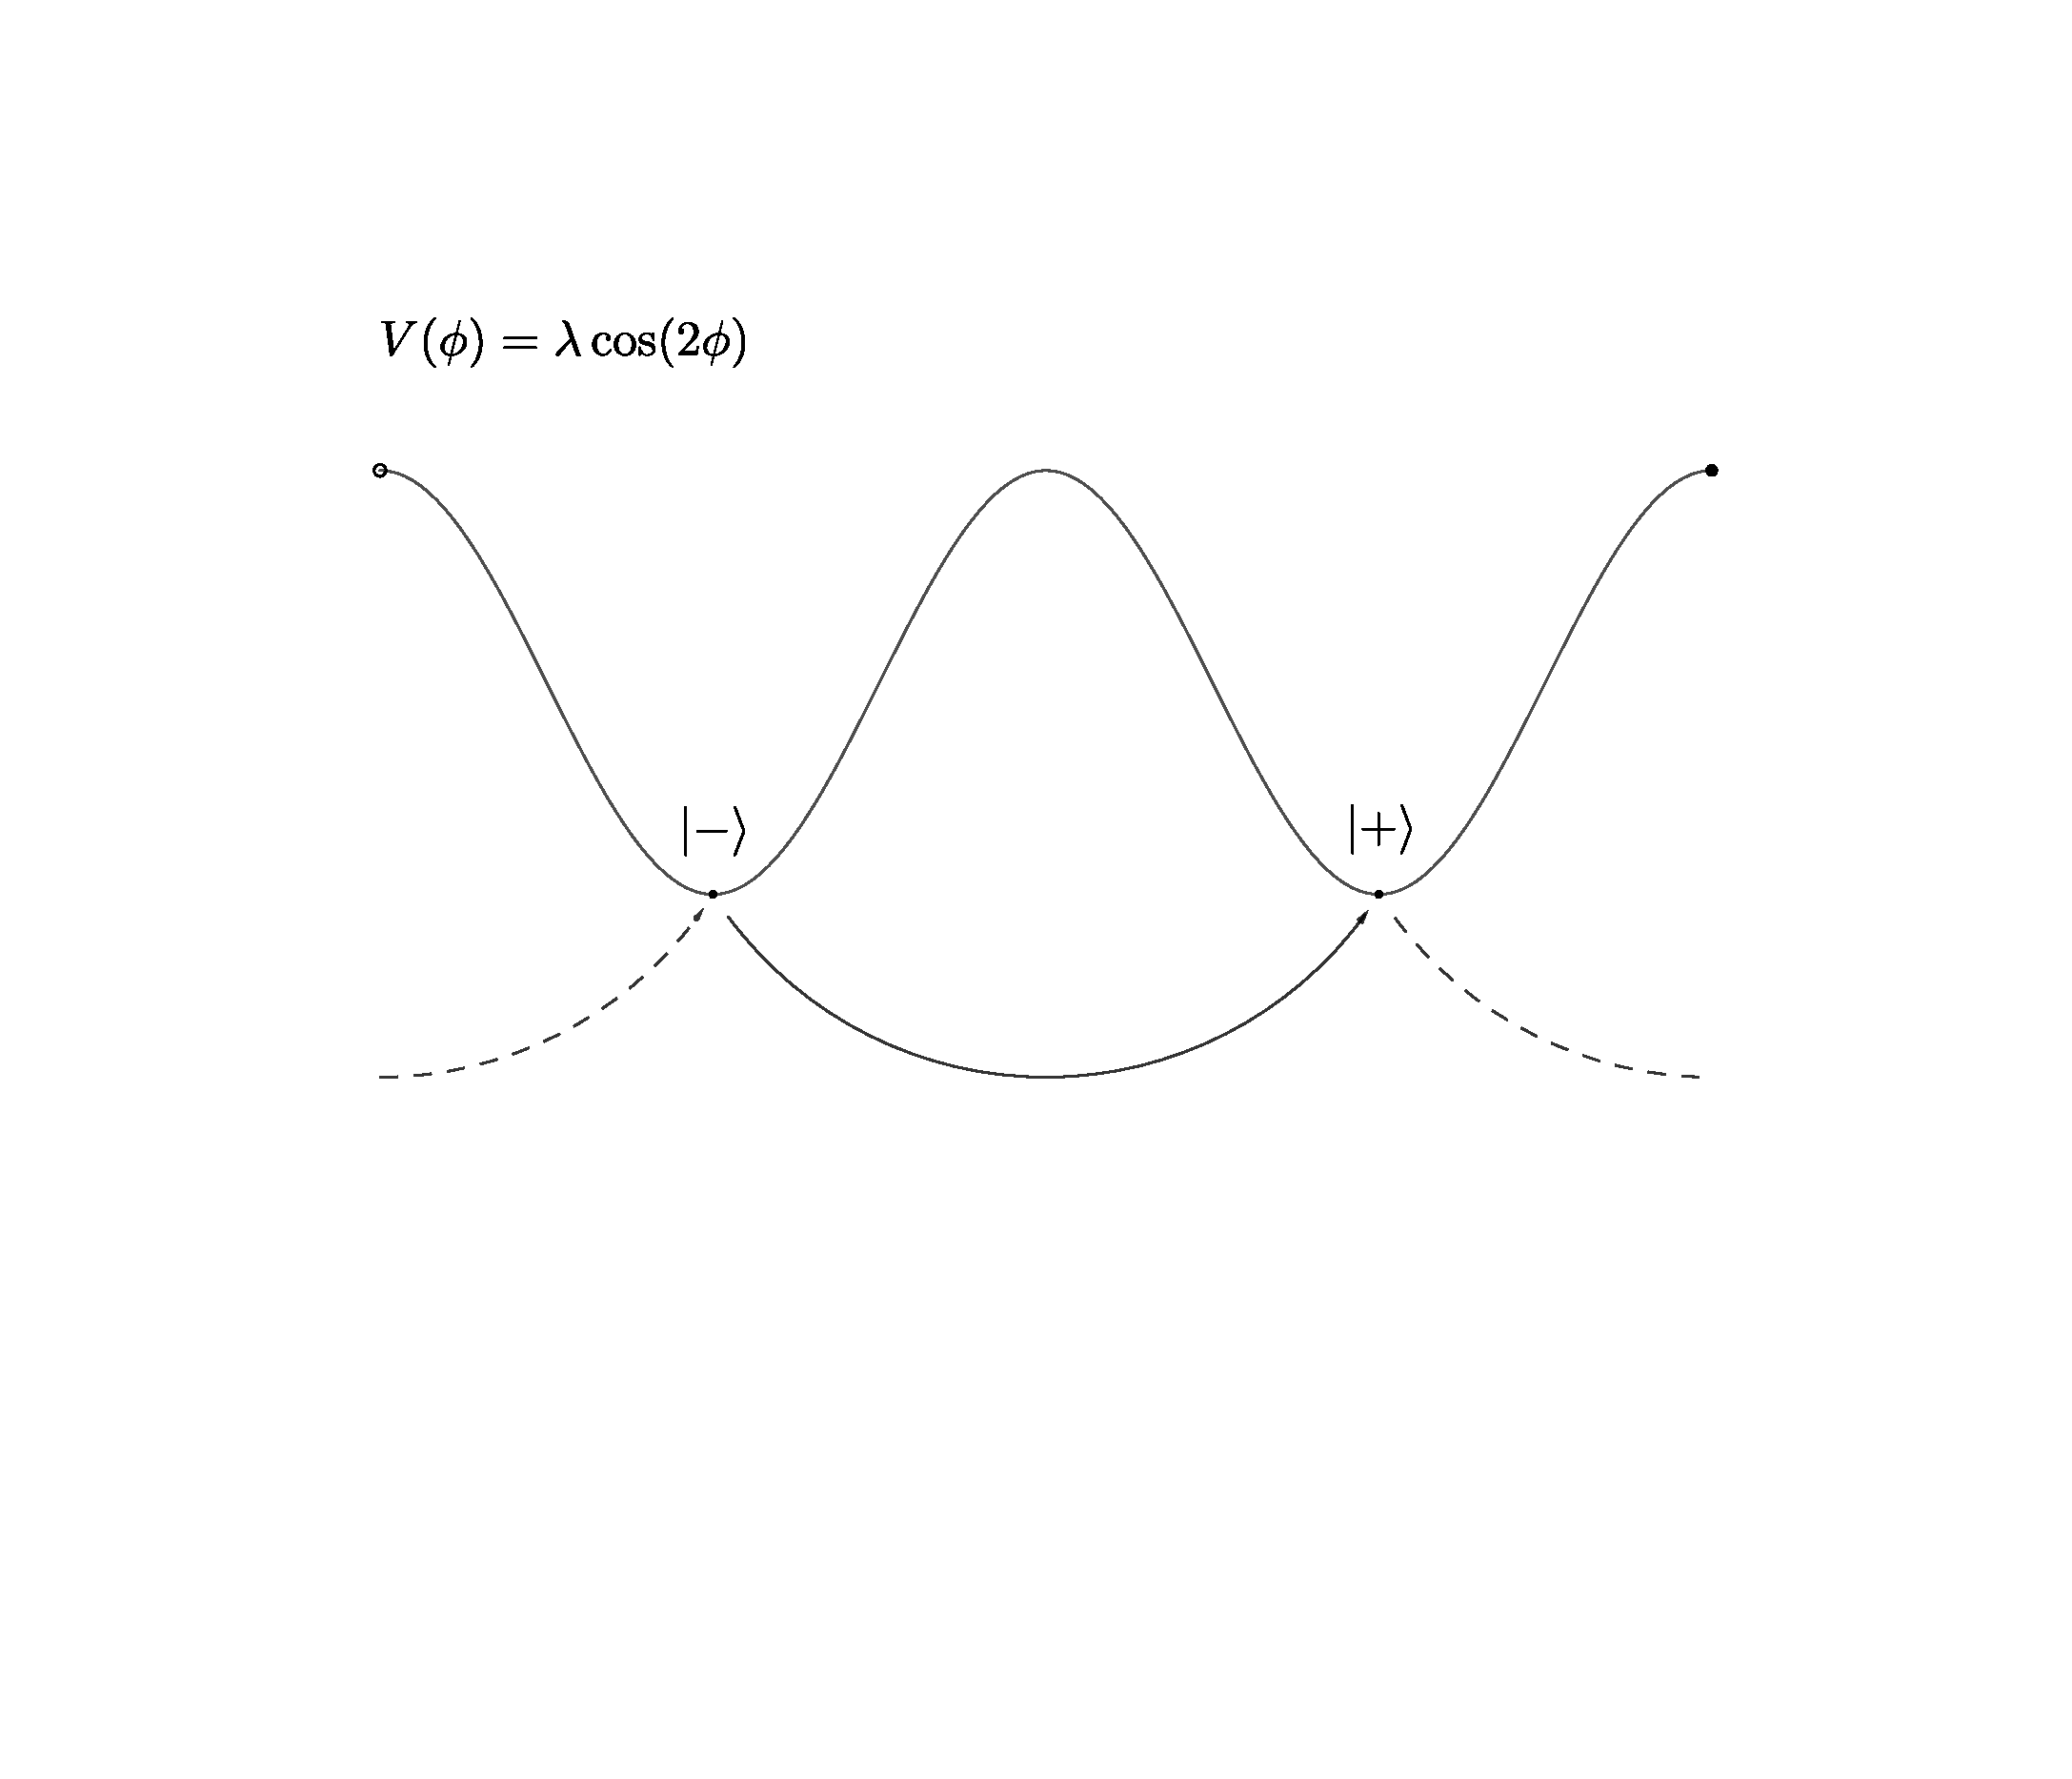
\includegraphics[trim={0cm 10cm 0cm 4cm}, clip, width=\textwidth]{instanton.pdf}
  	\caption{Tunneling effects between the two minima sitting in $+ = + \frac{\pi}{2}$ and $- = - \frac{\pi}{2}$. The thick and dashed lines represent respectively the instanton and the anti-instanton configuration}
   	\label{inst}
\end{figure}

\subsection{Example 3 Maxwell Theory}
Let's consider the Maxwell Lagrangian on a $D$ dimensional manifold $\mathcal{M}$
\begin{equation}
    S_{\text{Maxwell}} = \frac{1}{4 e^2} \int_{\mathcal{M}} F \wedge \star F 
\end{equation}
In absence of sources, it holds
\begin{equation}
    \begin{aligned}
       \text{Bianchi Identity}&\, dF=0\\
        \text{Equations of Motion}&\, d \star F=0
    \end{aligned}
\end{equation}
In the following, we will consider the simplified situation of a 4 dimensional spacetime of the form $\mathcal{M}=\mathbb{R}\times \mathcal{X}$ for some (compact) Riemannian manifold $\mathcal{X}$ (Spacetimes which admits this structure are called \textbf{globally hyperbolic}). Furthermore, for simplicity we will also assume that the the metric is independent of time.\footnote{More properly, we will assume that the metric admits a timelike Killing vector field which induces canonically a notion of time}\\


We can build two $1$-form symmetry as the integral of $\star F$ over a codimension $2$ submanifold $\Sigma$
\begin{defn}{Electric 1-form symmetry}{}
The topological operator associated to $\star F$
    \begin{equation}
    U_{\alpha}(\Sigma) = \exp(i \frac{\alpha}{2e^2} \int_{\Sigma} \star F)
    \label{eq:TopEleMaxwell}
\end{equation}
is called \textbf{electric 1-form symmetry} and the associated symmetry will be indicated as $U(1)^{(1)}_e$
\end{defn}

Integrals of $\int_{\Sigma} \star F$ and $\int_{\Sigma} F$ can be physically interpreted as respectively \textit{the electric} and \textit{the magnetic} flux crossing the surface $\Sigma \subset \mathcal{X}$. Indeed, due to the structure of $\mathcal{M}$, the electromagnetic tensor $F \in \Omega^2(\mathcal{M})$ can be expressed in a simplified form
\begin{equation}
    F=B-\dd{t}\wedge E
\end{equation} 
where $B=B(t)\in\Omega^2(\mathcal{X})$ and $E=E(t)\in \Omega^1(\mathcal{X})$ are respectively the \textbf{magnetic} and \textbf{electric field forms}. By choosing local coordinates on $\Sigma$, one can see that
\begin{equation}
    \int_{{\{t\}\times\Sigma}} F \,\,\, \text{and} \,\,\, \int_{{\{t\}\times\Sigma}} \star F
\end{equation}
measure respectively the magnetic and the electric flux crossing the surface $\Sigma$ at time $t$.

The $\U(1)^{(1)}_{e}$ symmetry is generated by the shift of the gauge field by a flat connection 
\begin{equation}
	A\rightarrow A+\lambda,\qquad \dd\lambda=0
\end{equation}
This is indeed a symmetry of the action since the connection $\lambda$ is flat. Moreover, is easy to see that this does not act on local operators being polynomials only in the curvature $F$. Indeed, in the pretty picture of topological operators, the $1$-form symmetry operator can be freely deformed past local insertions.\\
This symmetry acts non-trivially on extended operators known as \textit{Wilson lines}
\begin{defn}{Wilson Lines}{}
Given a curve $\gamma \subset \mathcal{M}$, for any integer $\mathbb{Z}$\footnote{If $A$ is a $U(1)$-connection/gauge field, in the second part of the proof of Thm.\ref{thm1}, it is shown that $W_{n}[\gamma]$ is a well defined object/gauge invariant if and only if $n \in \mathbb{Z}$ }, we define the Wilson line as
\begin{equation}
    W_n[\gamma]=\exp\qty(in\oint_\gamma A)
    \label{eq:Wilson1}
\end{equation}  
\end{defn}
The action of (\ref{eq:TopEleMaxwell}) on (\ref{eq:Wilson1}) can be easily seen in the following setup. Without loss of generality, take $D=4$ and consider a Wilson line in the $x$ direction. Put the topological operator later in time in the $y,z$ direction, orthogonal to the Wilson line. When the Wilson line passes the topological operator it will carry an additional phase measuring it's charge under the $\U(1)^{(1)}_{e}$. The adjoint action can be found by noting that $A_{x}$ and $F^{0 x}$ are canonically conjugate variables and therefore by using the canonical commutation relation one can find the operator action.The charge of the Wilson lines under this symmetry are completely classified by the holonomies of such Wilson line.\\


Observe that, due to the Bianchi identity, we also have another topological operator, implementing a "magnetic" $U(1)$ $(d-p)$-form symmetry
\begin{equation}
    U_\alpha\qty(\Sigma^{(d-p-1)})=\exp\qty(i\frac{\alpha}{2e^2}\int_\Sigma F)
\end{equation}
\begin{Jargon}{Gauging a Symmetry}{}
    Gauging a continuous symmetry $G$ (or $0$-form $G$ symmetry in our language) is an insertion in the Lagrangian of a \textit{minimal coupling term} 
    \begin{equation}
       \delta L_{\text{Int}} \doteq \tr(B \wedge \star J)
    \end{equation}
between the \textbf{background gauge connection for the symmetry} $B \in \Omega^{1}(\mathcal{M}) \otimes \mathfrak{g}$ and  \textbf{the conserved current} $j \in  \Omega^{1}(\mathcal{M}) \otimes \mathfrak{g}$ \textbf{associated to the symmetry} $G$ via \textit{Noether's theorem}. The background gauge connection $B$ has to considered a dynamical variable to be integrated over to compute the partition function $Z$\footnote{Notice that if we were interested only in proving the gaugability of a symmetry is sufficient to minimally couple the symmetry current $j$ with a \textit{static background field} and study the behaviour of the effective action $Z[B]$ under gauge transformations. }.  
\end{Jargon}

In analogy to the procedure of a gauging a symmetry ($0$-form symmetry), we can define the gauging procedure for a $p$-form symmetry
\begin{defn}{Gauging a p-form symmetry}{}
Gauging\footnote{This notion of gauging has been extended in \cite{Roumpedakis2022aik} taking into account the possibility to "complete" $\star j$ to a $k<d-p-1$ connection form and thus integrate the interaction on alower dimensional submanifold. This notion has been proven pivotal to construct higher symmetries from lower dimensional ones.}  a continuous $p$-form symmetry $G^{(p)}$ is an insertion in the Lagrangian of a \textit{minimal coupling term}
  \begin{equation}
       \delta L_{\text{Int}} \doteq \tr(B \wedge \star J)
    \end{equation}
between the \textbf{background gauge connection for the symmetry} $B \in \Omega^{d-p-1}(\mathcal{M}) \otimes \mathfrak{g}$ and  \textbf{the conserved current} $j \in  \Omega^{d-p-1}(\mathcal{M}) \otimes \mathfrak{g}$ \textbf{associated to the symmetry} $G^{(p)}$
\end{defn}


\subsection{Arising of Discrete Symmetries and their Gauging}
In the study of higher symmetries, we will need also to gauge a \textbf{discrete symmetry}. Let's consider the relevant case of multiplicative cyclic group $\mathbb{Z}_N$. This can be embedded in the $U(1)$ group.

In order to implement a $\mathbb{Z}^p_N$ gauge connection, we can add in the Lagrangian a Lagrange multiplier term which enforces the condition
\begin{equation}
    \exp(i N \int_{\Sigma} B) =1
\end{equation}
where $\Sigma$ is a dimension $p+1$ manifold. The term is
\begin{equation}
    \delta L_{\text{ghost}}[c, \lambda, B] \doteq \frac{i}{2 \pi} c \wedge ( N B - d \lambda)
\end{equation}
where $\lambda \in \Omega^p(\mathcal{M})$ and $c \in \Omega^{d-p-1}(\mathcal{M})$. \\
The lagrangian $\delta L_{\text{ghost}}[c, \lambda, B]$ is gauge invariant provided that
\begin{equation}
\begin{aligned}
    \lambda &\to \lambda + N \Lambda\\
    c &\to c
    \end{aligned}
\end{equation}
where as usual the Gauge transformation of the connection $B$ is defined as $B \to B + d \Lambda$. \\
If we integrate out $c$
\begin{equation}
    Z[\lambda, B] = \int d[c] e^{i S_{\text{Maxwell}} + i \delta S_{\text{int}}} \exp(\frac{i}{2 \pi} \int  c \wedge ( N B - d \lambda) ) = e^{i S_{\text{Maxwell}} + i \delta S_{\text{int}}} \delta(NB - d \lambda)
\end{equation}

\begin{thm}{}{}
\label{thm1}
Gauge equivalence classes of \textit{$U(1)$ flat connections $A$} over a manifold $\mathcal{M}$ are uniquely determined by their \textbf{holonomies/Wilson Lines}
\begin{equation}
    W_{\ell} \doteq \exp(i \alpha \oint_{\ell} A)
\end{equation}
where $[\ell] \in \pi_1(\mathcal{M})$ and $\alpha \in \mathbb{Z}$
\end{thm}

\begin{proof}
The spirit of the theorem is the following if we know what are the integrals on closed curves of a $1$-form $A$ we know completely the form $A$. The content of the theorem  is that for flat connections, \textit{the only non trivial informations are encoded in the holonomies}, i.e. in the integrals along non contractible cycles. \\
Let's show first that the map
\begin{equation}
    \begin{aligned}
 \pi(\mathcal{M}) &\to U(1)\\
 [\ell] &\mapsto \exp(i \alpha \oint_{\ell} A)
    \end{aligned}
\end{equation}
doesn't depend on the choice of the representative in each homotopy equivalence class. Let then $\ell$ and $\ell'$ be closed curves in $\mathcal{M}$ such that $[\ell] = [\ell']$. Thus, there exists a contractible loop $c$ such that $\ell = c * \ell'$. Computing the map on $\ell$
\begin{equation}
    \begin{aligned}
        \exp(i \alpha \oint_{\ell} A) &=   \exp(i \alpha \oint_{c * \ell'} A)\\
        &= \exp(i \alpha \oint_{c } A + i \alpha\oint_{\ell'} A)\\
        &= \exp(i \alpha \oint_{c } A) \exp(i \alpha\oint_{\ell'} A)\\  
    \end{aligned}
\end{equation}
We claim that if $[c]=[e]$ then, $c$ is the boundary of a $2$ dimensional submanifold $\Omega$\footnote{More precisely $c \in \Im (\partial: C_2 \to C_1)$ where $\partial$ is the \textbf{boundary operator} of the \textbf{singular homology} and $C_i$ are the \textbf{chains} of the homology (See Sec. \ref{hom} for a brief recap or \cite[Section 2.1]{Hat} for details)}
\begin{proof}
    If $c$ is homotopic to the constant path $e$, there exists a (continuous) map $F$
    \begin{equation}
    \begin{aligned}
        F: [0,1] \times S^1 &\to \mathcal{M}\\
            (t,s) &\mapsto F(t,s)
        \end{aligned}
    \end{equation}
    such that
    \begin{enumerate}
        \item $F(0,s) = c(s)$
        \item $F(1,s) = e(s)$
    \end{enumerate}
We can see from the the figure that $c$ is the boundary of $\Omega = \text{Graph}(F)$. Furthermore, by projecting the graph onto the $t=0$ section, it can be seen as an object homeomorphic to a disc $D$ (i.e. a $2$ dimensional ball).
\end{proof}
By the above claim, Stokes' theorem and flatness condition of the connection
\begin{equation}
    \exp(i \alpha \oint_c A) = \exp(i \alpha \oint_{\partial \Omega} A)  = \exp(i \alpha \int_{\Omega} dA) = 1
\end{equation}
This shows that holonomies/Wilson lines depends only on homotopy class of paths. Let's see now why, holonomies completely defines a gauge equivalent class of flat connections. \\

Let's be more precise on the meaning of gauge transformations of $A$. Let $\{U_{\alpha}\}_{\alpha}$ be a covering of $\mathcal{M}$ and $\{e_{\alpha}: U_{\alpha} \to \mathbb{C} \}_{\alpha}$ be a set of local sections of a line bundle $\mathcal{L} \to \mathcal{M}$ (which has to be seen as the associated line bundle to the $U(1)$ principal bundle over $\mathcal{M}$). Gauge transformations are changes of local frames on $U_{\alpha \beta } \doteq U_{\alpha} \cap U_{\beta}$
\begin{equation}
    g_{\alpha \beta}: U_{\alpha \beta} \to U(1) 
\end{equation}
such that
\begin{equation}
    e_{\alpha} = g_{\alpha \beta} e_{\beta}
\end{equation}
In order a have a well defined covariant derivative
\begin{equation}
    D e_{\alpha} = d  e_{\alpha} + i A_{\alpha} \wedge e_{\alpha}
\end{equation}
$A$ transforms consequently as
\begin{equation}\label{gauge}
    A_{\alpha} = g_{\alpha \beta} A_{\beta} g_{\alpha \beta}^{-1} -  i d  g_{\alpha \beta} g_{\alpha \beta}^{-1}
\end{equation}
Locally, we can find some $\lambda_{\alpha \beta}:U_{\alpha \beta} \to S^1$ such that $g_{\alpha \beta} = e^{i \lambda_{\alpha \beta}}$, so \eqref{gauge} can be rewritten as
\begin{equation}
    A_{\alpha} = A_{\beta}  + d \lambda_{\alpha \beta}
\end{equation}
Notice that this implies that $A$ is \textbf{not a well defined} element of $\Omega^1(\mathcal{M})$. In general, for any partition $\{U_{\alpha}\}$ of $\mathcal{M}$, $A$ is given by a
\begin{enumerate}
    \item \textbf{Set of Local Expressions} $A_{\alpha} \in \Omega^1(U_{\alpha})$
    \item \textbf{Set of Gauge transformations} $g_{\alpha \beta} :U_{\alpha \beta} \to U(1)$ satisfying the condition
    \begin{equation}\label{co}
        g_{\alpha \beta} g_{\beta \gamma} = g_{\alpha \gamma} 
    \end{equation}
    for $U_{\alpha} \cap U_{\beta} \cap U_{\gamma} \doteq U_{\alpha \beta \gamma} \neq \emptyset$
    \item \textbf{Transformation Laws} $ A_{\alpha} = g_{\alpha \beta} A_{\beta} g_{\alpha \beta}^{-1} -  i d  g_{\alpha \beta} g_{\alpha \beta}^{-1}$  
\end{enumerate}

Suppose we make a gauge transformation of $W_{\ell}$
\begin{equation}
\begin{aligned}
    W_{\ell} &\to W_{\ell} \prod_{i=1}^N \exp(i \alpha \oint_{\ell} d \lambda_{\alpha_i \beta_i})
    \end{aligned}
\end{equation}
where $\{\alpha_i\}_{i=1}^N$ and $\{\beta_i\}_{i=1}^N$ are respectively the indices associated to the partition used in the first and in the second computation of $W_{\ell}$. We can refine both partitions $\{U_{\alpha_i}\}_{\alpha_i}$ and $\{U_{\beta_i}\}_{\beta_i}$ in order to get a covering $\{U_{\alpha_i  \beta_j}\}_{\alpha_i \beta_j}$ formed by $2$ to $2$ intersections. Then
\begin{equation}
    \sum_{i,j=1}^N   \oint_{\ell} d \lambda_{\alpha_i \beta_j} = \sum_{i,j=1}^N \lambda_{\alpha_i \beta_j}|_{\ell \cap \partial U_{\alpha_i \beta_j}} = 2 \pi n
\end{equation}
where we have used the fact that from \eqref{co} we can deduce
\begin{equation}
    \lambda_{\alpha \beta} + \lambda_{\beta \gamma} = \lambda_{\alpha \gamma} + 2 \pi n
\end{equation}
for some $n \in \mathbb{N}$\footnote{Another way to argue this is by recognising the map
\begin{equation}
    \ell \to \oint_{\ell} d \lambda
\end{equation}
as an homotopy equivalence classes of mapping from $S^1 \to S^1$ (i.e. elements of $(\pi_1(S^1)= \mathbb{Z}$) which are catalogued by \textbf{winding numbers} (See \cite[Section 2.1.2]{percacci}) }. Holonomies are thus gauge invariant which completes the proof.  
\end{proof}
\begin{rem}
    For an $\mathbb{R}$ connection, \eqref{co} reduces to

    \begin{equation}
    \lambda_{\alpha \beta} + \lambda_{\beta \gamma} = \lambda_{\alpha \gamma} 
\end{equation}
since
\begin{equation}
    \lambda_{\alpha \beta}: U_{\alpha \beta}  \to \mathbb{R}
\end{equation}
Thus, there is \textit{no holonomy associated to the connection $A$}. This implies in particular that $A \in \Omega(\mathcal{M})$ or in other words it is a \textit{well defined global $1$-form over $\mathcal{M}$}. \\

Furthermore the proof has shown that \textit{$\alpha$ is forced to be integer} if we insist for the \textbf{Wilson line} to be \textbf{gauge invariant}. This \textit{relied} on the \textbf{existence of a non trivial cycle on the manifold} $\mathcal{M}$ \textit{and} a \textbf{non trivial topology of the gauge group} $G$. Thus for an $\mathbb{R}$ connection over any manifold $\mathcal{M}$ or for any $G$ connection on $\mathcal{M} = \mathbb{R} \times \mathbb{R}^N$ (or more generally on $\mathcal{M} = \mathbb{R} \times \mathcal{X}$ with $\mathcal{X}$ simply connected Riemannian Manifold), $\alpha$ can be any real number. \\

If we interpret a Wilson line as the \textit{universe line} of a $G$ charged particle (with $G$-charge $\alpha$), we can regard this remark as a statement regarding the \textbf{quantization of charge}.    
\end{rem}

\subsection{Homology, cohomology and gauge fields}
In this section we will give the necessary background to understand how to formlise the insertion of topological operators in a QFT. A particularly natural way of prescribing the insertion of defects on a given manifold is given by simplicial homology. Here we'll give some basic definitions for such homology theory.\\

\subsubsection{Sequences}
We start from some preliminary definitions
\begin{defn}{Exact Sequence}{}
    Let \textit{$\{G_i\}_{i \in \mathbb{Z}}$} be a \textit{collection of groups} and \textit{$\{m_i: G_i \to G_{i+1}\}_{i \in \mathbb{Z}}$} a \textit{collection of group homomorphisms}, we say that the sequence:
\begin{equation}\label{exact}
      \cdots \xrightarrow[]{m_{i-2}} G_{i-1} \xrightarrow[]{m_{i-1}} G_i \xrightarrow[]{m_i}   G_{i+1} \xrightarrow[]{m_{i+1}} G_{i+2} \xrightarrow[]{m_{i+2}} \cdots
\end{equation}
is \textbf{exact}, if
\begin{equation*}
        \ker m_{i+1}= \Im m_i \,\,\,\forall i \in \mathbb{Z}
\end{equation*}
Notice that this implies
\begin{equation*}
          m_{i+1} \circ m_i  = \text{Id}
\end{equation*}
If the exact sequence has only $3$ non trivial groups $H, \Gamma, G$
 \begin{equation*}
      \{e\} \xrightarrow[]{} H  \xrightarrow[]{f} \Gamma \xrightarrow[]{g}   G \xrightarrow[]{} \{e\}
    \end{equation*}
it is called \textbf{short exact sequence}. Usually, the trivial group ${e}$ is substituted by a $0$ for additive notation, or by a ${1}$ for multiplicative notation.
\end{defn}
For short exact sequences it holds the following
\begin{thm}{$1^{\text{st}}$-Homorphism theorem}{}
Given a short exact sequence: 
\begin{equation*}
      \{e\} \xrightarrow[]{} H  \xrightarrow[]{f} \Gamma \xrightarrow[]{g}   G \xrightarrow[]{} \{e\}
    \end{equation*}
then
\begin{equation*}
    G \simeq  \Gamma / H
\end{equation*}
\end{thm}


\begin{proof}
Let's do a couple of observations: 
    \begin{enumerate}
        \item $\ker f = \{e\} $
        \item $\Im g = G$
        \item $\Im f = \ker g$
    \end{enumerate}
We can then roughly see $H$ as a subgroup of $\Gamma$ (more precisely $H$ is isomorphic to the subgroup $f(H)$ of $\Gamma$). Let's argue that $f(H)$ is a normal subgroup of $\Gamma$. This follows from the third equality and the fact that \textit{kernels of group homomorphisms are always normal subgroups}. \\
Let's build a short exact sequence:
\begin{equation*}
      \{e\} \xrightarrow[]{} H  \xrightarrow[]{f} \Gamma \xrightarrow[]{\pi}   \Gamma / f(H) \xrightarrow[]{} \{e\}
\end{equation*}
where now $\Gamma/ f(H)$ is a well defined group since $f(H)$ is normal. Since the diagram\\
\adjustbox{scale=1, center}{
\begin{tikzcd}
\{e\} \arrow{r}{} \arrow[swap]{d}{\text{Id}} & H \arrow{r}{f} \arrow[swap]{d}{\text{Id}} &\Gamma \arrow{r}{g} \arrow[swap]{d}{\text{Id}}  &G  \arrow{r}{} \arrow[swap]{d}{\phi} &\{e\} \arrow{d}{\text{Id}}\\
\{e\} \arrow{r}{}  & H \arrow{r}{f}   &\Gamma \arrow{r}{\pi}    &\Gamma/f(H)  \arrow{r}{} &\{e\}  \\
\end{tikzcd}}
commutes, $\phi: G \to \Gamma/f(H)$ (which is uniquely defined by the commutativity of the diagram and the exactness of the sequences) is an isomorphism. 
\end{proof}



\subsubsection{Simplicial Homology}\label{hom}
More or less, homology is the classification of closed manifolds modulo boundary. In simplicial homology, the basic objects are $n$-\textbf{Simplices}  which are very simple combinatorial objects.\\
A $0$-simplex $\Delta^{0}$ is just a point, a $1$-simplex $\Delta^{1}$ is a line whose boundary are two $\Delta^{0}$. One can go on: a $2$-simplex $\Delta^{2}$ is a triangle whose boundary is made by $\Delta^{1}$ and vertices by $\Delta^{0}$, and so on. More generally
\begin{equation}
	\Delta^{n}\text{ has }(n+1)\text{ vertices and the faces are made of }\Delta^{n-1}
\end{equation}
Consider now an arbitrary ordering of the vertices and indicate them by $\{i\}$. Take a $3$-simplex $\Delta^{3}$ (a tetrahedron), this has
\begin{equation}
\begin{split}
	\Delta^{3}&=[0123]\\
	\Delta^{2}&=[123],[023],[013],[012]\\
	\Delta^{1}&=[01],[02],[03],[12],[13],[23]\\
	\Delta^{0}&=[0],[1],[2],[3]
\end{split}
\end{equation}
We would like now to \textit{triangulate} our manifold with simplices. First let us define some objects on simplicies
\begin{defn}{$p$-chain}{}
	A $p$-chain $\gamma\in C_{p}(\Delta^{n})$ is a formal sum
	\begin{equation}
		\gamma=\sum_{[\ldots]}c_{i_{0}i_{1},\ldots,i_{p}}[i_{0}i_{1}\cdots i_{p}]
	\end{equation}
	where the coefficients are elements of $\bbZ$ or, more generally, any abelian group $\bbA$ (this is just what we need, of course the coefficients can be valued in more complicated objects). The sum is carried on every possible simplex with $p+1$ entries.\\
	$C_{p}(\Delta^{n})$ is a free Abelin group of rank $p$, where the group structure is just given by the group structure of the coefficients.
\end{defn}
As an example, consider a $2$-dimensional manifold. A $1$-chain is just a curve when the coefficients are in $\bbZ$, and a colored curve when the coefficients are in $\bbA$, where every side has an associated element of the abelian group stuck to it. We are going to interpret these elements as the insertion of a defect along such side. Physically a $p$-chain is an assignment of a \textbf{consistent} network of defects.\\
To have a good theory of homology, we need to construct a boundary operator. For simplicies this is just given by 
\begin{defn}{Boundary operator}{}
	The \textit{boundary homeomorphisim} is an homeomorphism between chains
	\begin{equation}
		\partial:C_{j}(\Delta^{n})\rightarrow C_{j-1}(\Delta^{n})
	\end{equation}
	which acts on simplices as
	\begin{equation}
		\partial[i_{0}\cdots i_{j}]=\sum_{k=0}^{j}(-1)^{k}[i_{0},\cdots,i_{k-1},i_{k+1},\cdots i_{j}]
	\end{equation}
	so it acts on $p$-chains by linearity as
	\begin{equation}
		\partial\gamma=\sum_{[\ldots]}c_{i_{0},\ldots,i_{p}}\partial[i_{0},\cdots,i_{p}]
	\end{equation}
	Notice that $\partial^{2}=0$.
\end{defn}
Now we would like to triangulate our manifold. To do so we define the following
\begin{defn}{Simplicial complex}{}
	Given an $n$-dimensional oriented manifold $X$, a simplicial complex $\Delta (X)$ is a finite set of simplicies in $\bbR^{n}$ such that one has a collection of maps $\sigma_{\alpha}^{p}:\Delta^{p}\rightarrow X$ for $p=0,\ldots,n$ which are
	\begin{enumerate}
	\item Injective
	\item $\sigma_{\alpha}^{p}\Big |_{\text{face}}\in \sigma^{p-1}_{\beta}$
	\end{enumerate}
meaning that given a simplex $\sigma^{p}$ in $\Delta(X)$, also the faces of the simplex are in $\Delta(X)$ and that every non-empty intersection of two simplices is a face of both.
\end{defn}
Notice that not every manifold in $n>3$ is triangulable.\\

A $p$-chain on $\Delta(X)$ is just given by the formal sum
\begin{equation}
	 \gamma=\sum_{\beta}c_{\beta}\sigma^{p}_{\beta},\qquad c_{\beta}\in\bbA
\end{equation}
and the boundary operator acts as
\begin{equation}
	\partial \gamma=\sum_{\beta}c_{\beta}\partial_{p}\sigma_{\beta}^{p}.
\end{equation}
\begin{defn}{Chain Complex}{}
	Given a simplicial complex $\Delta(X)$ there exists a sequence of abelian groups and homeomorphisms
	\begin{equation}
		0\xhookrightarrow{\iota} C_{n}(\Delta(X),\bbA)\xrightarrow{\partial_{n}} C_{n-1}(\Delta(X),\bbA),\xrightarrow{\partial_{n-1}}C_{n-2}(\Delta(X),\bbA)\rightarrow\cdots
	\end{equation}
	The first map is the inclusion map. This sequence is called \textbf{chain complex} and is referred to as $C(X)$.
\end{defn}
Given that $\partial^{2}=0$ is a boundary operator, the chain complex lets us define an homology on $X$
\begin{equation}
	\HH_{j}(\Delta(X),\bbA)=\frac{\ker \partial_{j}}{\Im \partial_{j-1}}
\end{equation}
which essentially classifies closed chains up to boundaries ($\partial\gamma=0$ but $\gamma\neq\partial\tilde\gamma$).

Consider for example the $2$-torus $T^{2}\simeq S^{1}\times S^{1}$. This can be triangulated as follows
\begin{equation}
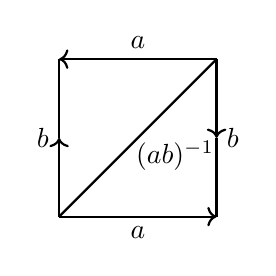
\begin{tikzpicture}[thick]
  \draw[->](0,0)--(0,1) node[anchor=east] {$b$};
  \draw[-](0,1)--(0,2);
  \draw[<-](0,2)--(1,2) node[anchor=south] {$a$};
  \draw[-](1,2)--(2,2);
  \draw[->](2,2)--(2,1)node[anchor=west] {$b$};
  \draw[-](2,1)--(2,0);
  \draw[<-](2,0)--(1,0) node[anchor=north] {$a$};
  \draw[-](1,0)--(0,0);
  \draw[-](0,0)--(2,2) node[yshift=-35, xshift=-15] {$\tiny (ab)^{-1}$};
\end{tikzpicture}
\end{equation}
Here we have two $0$-chains $[a],[b]$ which are closed but $[(ab)^{-1}]=-[a]-[b]+\partial[\ldots]$. Therefore $H_{1}(T^{2})=\bbZ\oplus\bbZ$.

If we label the edges with the right group elements from $\bbA$ (so we put defects on the edges) and take a chain, we see that the closeness condition implies the group law
\begin{equation}
	\gamma=a[10]+b[20]+c[03]+\cdots
\end{equation}
then
\begin{equation}
	\left.\partial\gamma\right|_{[0]}=(a+b-c)[0]=0\implies a+b=c
\end{equation}
So a closed chain is in one-to-one correspondence with defects carrying group law. A chain $\gamma\in C_{d-p-1}(X,\bbA)$ is closed, then $\gamma$ corresponds to a $p$-form symmetry.

We also need to mod out for boundaries. Boundaries are nuclated whenever we have a loop in the network since they have to be closed by definition. Therefore, when we want to talk about defects, we not only require them to be closed but also mod out by nucleation which requires them to be in some homology group.

\section{Chern-Simons theory}
This chapter is basically a relaboration and expansion of \cite[Chapter 2]{Moor} which has also been covered in a four lectures series at TASI by Greg Moore on CS-theory. 

\subsection{$U(1)$-Chern Simons Theory}
A Chern-Simons theory is a Gauge theory with the following inputs
\begin{enumerate}
    \item A \textbf{Compact Lie group $G$}\footnote{Generalizations to Finite groups will be discussed In section \ref{ZNCS}}
    \item An \textbf{orientable $3$-Manifold} $\mathcal{M}_3$
    \item A \textbf{$G$-Principal Bundle $P \to \mathcal{M}$} with local connection $A_i \in \Omega(U_i) \otimes \mathfrak{g}$ ($\cup_{i} U_i = \mathcal{M}_3$)
\end{enumerate}
If the bundle $P \to \mathcal{M}_3$ can be trivialized\footnote{$P \simeq G \times \mathcal{M}_3$}, $\{A_i\}$ can be consistently patched together in a well defined global $\mathfrak{g}$-valued $1$-form $A$. The Chern-Simons action is:
\begin{equation}
    S_{\text{Chern-Simons}} = \frac{k}{8 \pi^2} \int_{\mathcal{M}_3} \text{Tr}(A \wedge d A + \frac{2}{3} A \wedge A \wedge A)
\end{equation}

\subsection{Quantization}
\subsubsection{Quantization Procedures}

\subsubsection{Mathematical Aside: Moment Map and Symplectic reduction}
Let $(\mathcal{M}, \omega)$ be a \textbf{symplectic manifold}. We are interested in studying the action $\phi_{(\cdot)}$ of some Lie group $G$ on $\mathcal{M}$ which preserves the symplectic form $\omega$:
\begin{equation}
	\label{sy}
    \phi_g^*(\omega) = \omega
\end{equation}
for any $g \in G$. Flows of this type are called \textbf{symplectomorphisms}. A simple example of those actions is provided by \textbf{Hamiltonian Vector Field} $X_f \in \Gamma(T \mathcal{M})$ associated to any $f \in C^{\infty}(\mathcal{M})$. Those vector fields are defined by the condition:
\begin{equation}
    \omega(X_f,\cdot) = \dd f
\end{equation}
which can be read in coordinates $(x^1,\cdots,x^{2n})$, as
\begin{equation}
    \omega_{ij} (X_f)^i = \partial_j f \to X_f^i = \omega^{ij} \partial_j f 
\end{equation}
where $\omega^{ij} \in \Gamma(T \mathcal{M} \otimes T \mathcal{M} )$ such that $\sum_j \omega^{ij} \omega_{jk} = \delta^{i}_k$. If we consider the group of diffeomorphisms generated by $X_f$, $\Phi_{X_f}^t$ ($t \in \mathbb{R}$), the condition \eqref{sy} is indeed satisfied because at any point $p \in \mathcal{M}$
\begin{equation}
   \mathcal{L}_{X_f} (\omega) = d \omega(X_f, \cdot) +  \cancel{(d \omega)}(X_f, \cdot , \cdot) = d^2 f =0
\end{equation}

In general, if $\xi \in \Gamma(T \mathcal{M})$ is the generator of the one group-parameter of symplectomorphism $\phi_{\exp(t T)}$ along some direction given by $T \in \mathfrak{g}$, using the same reasoning as above, it holds that:
\begin{equation}
    d \omega(\xi, \cdot) =0
\end{equation}
If $H^1_{\text{dR}}(\mathcal{M})= \{0\}$, then we can find a function $\mu(T) \in C^{\infty}(\mathcal{M})$ such that
\begin{equation*}
    \dd \mu(T) = - \omega(\xi, \cdot)
\end{equation*}
$\mu(T)$ is called the \textbf{charge} associated to the symmetry generated by the vector field $\xi$, because it generates $\phi_{\exp(t T)}$. Indeed
\begin{equation}
    \{ \mu(T), f\} = \omega^{ij} \partial_i \mu(T)\partial_j f = - \omega^{ij} \omega_{ik} \xi^i \partial_j f = \delta^j_k \xi^i \partial_j f = \xi^j \partial_j f = \xi(f) = \mathcal{L}_{\xi}(f)
\end{equation}
In more formal terms
\begin{defn}{Momentum Map}{}
   A Momentum Map is a linear assignment
  \begin{equation}
  \begin{aligned}
  	 \mu:  \mathfrak{g} &\to C^{\infty}(\mathcal{M})\\
	T &\mapsto \mu(T)
    \end{aligned}
\end{equation}
such that
\begin{equation}
     \phi_g^* \mu = \text{Ad}^*_g \mu
\end{equation}
where $\text{Ad}^*_g$ is the \textbf{coadjoint action} of $G$ on $\mathfrak{g}^*$ defined by
\begin{equation}
    \left \langle \text{Ad}^*_g \mu , T \right \rangle = \left \langle \mu , \text{Ad}_g T \right \rangle
\end{equation}
Equivalently, $\mu \in  C^{\infty}(\mathcal{M}) \otimes \mathfrak{g}^*$ by usual identification
\begin{equation}
    \left \langle \mu, T \right \rangle = \mu(T)
\end{equation}
\end{defn} 
Let's see some examples of momentum map.

\subsection{$\mathbb{Z}_n$-Chern Simons theory}\label{ZNCS}

\section{The power of symmetry}
We will state a lot of QM examples with very formal language, which will help understand the fancy language also for the fancier examples. Start with very limited definition of symmetry: a global symmetry means having a unitary operator $U$ that commutes with the hamiltonian $UH=HU$ (also anti-unitary for time reversal but ok). The second condition is that the operators are in a faithful linear (acts like an ordinary rep, not up to phases like states) representation (there is no symmetry op. that acts trivially on everything) of the symmetry group. 

Every op. $O_{i}$ is mapped as 
\begin{equation}
	O_{i}\rightarrow U O_{i}U^{-1}=\sum_{j}R_{ij}(U)O_{j}
\end{equation}
where $R$ is the representation matrix of the symmetry group.

The modern way to talk about symmetry is to pretend that we couple the system to background gauge fields for the symmetry (it is not gauge, is global, acts on Hilbert space and operators). We consider the system as one point in a family of theories labelled by a background gauge field. The object of interest is 
\begin{equation}
	Z(A)=\int e^{-S(A)}
\end{equation}
where $A$ is a vector potential to the symmetry, for example $\U(1)$, and does not have to satisfy any classical eom. Then we ask what happens under a gauge transformation $A\rightarrow A^{g}$, is the partition function gauge invariant? It could happen that
\begin{equation}
	Z(A^{g})=Z(A)e^{-i\omega(A,g)}
\end{equation}
maybe we should add some terms to the action to get rid to that phase. If it is not possible, than we say that there is an anomaly. This has nothing to do with field theory, fermions and whatever, this is the minimal way of thinking about it.

The simplest example is the following: a single qbit or equivalently a $2$-level system or a complex fermion in QM
\begin{equation}
	i\int\psi^{\dagger}\partial_{t}\psi
\end{equation}
What is the global symmetry? Maybe a $\U(1)$ that rotates the fermions, but also charge conjugation $\bbZ_{2}$ and together they give $\OO(2)$. Option number two, we have a 2 dimensional Hilbert space so we can perform any $2\times 2$ commutes with the hamiltonian which is $H=0$ and so one might think that the symmetry is $\U(2)$. But we need to consider that the representation should be linear so we have to mod out by a $\U(1)$ phase of the projective representation on states $\U(2)/\U(1)=\SO(3)$. Notice that the symmetry is bigger than before. This is happens usually since the lagrangian does not exhibit the full symmetry of the system (this phenomenon is known as quantum symmetry).

Symmetries act projectively on the Hilbert space: we have a symmetry operator
\begin{equation}
	S(\vec{r})=e^{i\vec{r}\cdot\vec{s}},\qquad \vec{s}=\frac{1}{2}\vec{\sigma}
\end{equation}
this is how the $\SU(2)$ is realized on the Hilbert space. Since the action is by conjugation, we ask what are the conjugacy classes of $\SO(3)$. We limit ourselves
\begin{equation}
	g(\xi)=e^{i\xi s^{z}},\qquad g(\xi)\sim g(-\xi),\qquad g(\xi+2\pi)=-g(\xi)
\end{equation}
The action on the Hilbert space is with the minus which means that the symmetry is realized by the double cover $\SU(2)$. Notice that the adjoint action on the operators does not see the minus sign.

Now we take a gauge field $A$ for the $\SO(3)$ symmetry (it only has a time component in QM) and pick a gauge such that $A$ does not depend on $t$ (we take euclidean time)
\begin{equation}
	Z(\xi)= \Tr e^{-\beta H} g(\xi)=2\cos\qty(\frac{\xi}{2})
\end{equation}
since we have two states with opposite spin and the Hamiltonian is zero. This works for $Z(-\xi)=Z(\xi)$ but $Z(\xi+2\pi)=-Z(\xi)$. But what if we use
\begin{equation}
	g(\xi)=e^{i\xi s^{z}}\rightarrow e^{i\xi(s^{z}+\frac{1}{2})}
\end{equation}
by doing this there is not the minus sign anymore. But now I messed up the initial formula for $Z(\xi)$. Such a redefinition is called adding a counterterm and the freedom of moving the anomaly around is the freedom of adding counterterms. So here we cannot satisfy the full symmetry $\SO(3)$.

Consider now another example: the rotor. We start with the lagrangian
\begin{equation}
	L=\frac{1}{2}\dot{q}^{2}+\frac{\theta}{2\pi}\dot{q},\qquad q\simeq+2\pi
\end{equation}
the global symmetries are
\begin{equation}
\begin{split}
	&\U(1):q\rightarrow q+\alpha,\qquad\text{Is not }\bbR\text{ since }q\text{ is circle valued}\\
	&\bbZ_{2}:q\rightarrow -q,\quad \theta=0 \mod \pi
\end{split}
\end{equation}
These two combine into
\begin{equation}
	\OO(2)=U(1)\rtimes\bbZ_{2}
\end{equation}
so that $\bbZ_{2}$ acts on $\U(1)$. Let us do some QM
\begin{equation}
	p=\dot{q}+\frac{\theta}{2\pi}
\end{equation}
and
\begin{equation}
	H=p\dot q-L=\frac{1}{2}\qty(p-\frac{\theta}{2\pi})^{2}
\end{equation}
and the eigenvalues of $p\in \bbZ$ since $q$ is circle valued. The spectrum of the hamiltonian is
\begin{equation}
	E_{n}=\frac{1}{2}\qty(n-\frac{\theta}{2\pi})^{2}
\end{equation}
where we have degenerate states at $\theta=\pi,3\pi,\ldots$. Let us go over the simmetries
\begin{equation}
\begin{split}
	&q\rightarrow q+\alpha, \qquad\text{charge }Q=P\\
	&q\rightarrow RqR^{-1}=-q\\
	&RQR^{-1}=R(\dot{q}+\frac{\theta}{2\pi})R^{-1}=-Q+2\frac{\theta}{2\pi}
\end{split}
\end{equation}
For $\theta=2\pi$ we can redefine the charge $Q\rightarrow Q-\frac{\theta}{2\pi}$ but for $\theta=2\pi$ I cannot do it. For $\theta=0\mod 2\pi$ the symmetry is $\OO(2)$ and is realized linearly but for $\theta=\pi\mod 2\pi$ the symmetry is anomalous, is still $\OO(2)$ but is realized projectively. 

In terms of gauge fields
\begin{equation}
	L=\frac{1}{2}\qty(\dot{q}+A)^{2}+\frac{\theta}{2\pi}\qty(\dot{q}+A)+k A
\end{equation}
where the last part is a Chern-Simmons term in QM. Choose a gauge where $A$ is constant and compute the partition function: for $\theta=\pi$ in euclidean the only gauge invariant information is the following 
\begin{equation}
	e^{i\oint A_{euc}}=e^{i\xi}
\end{equation}
and compute
\begin{equation}
	Z(\xi)=\Tr e^{-\beta H}e^{i\xi (n+k)}=\sum_{n=-\infty}^{\infty}e^{-\frac{\beta}{2}\qty(n+\frac{1}{2})^{2}}e^{i\xi(n+k)}
\end{equation}
Moreover
\begin{equation}
	Z(\xi+2\pi)=Z(\xi),\qquad Z(-\xi)=Z(\xi)e^{-i(2k+i)\xi}
\end{equation}
so it acquires a phase which depends on the background gauge field $\xi$. So the $\bbZ_{2}$ is anomalous and is not realised properly. What are we going to do about it? We have many options
\begin{enumerate}
	\item That's it, it is what it is, $k\in\bbZ$
	\item Set $k=-1/2$. Now the $\bbZ_{2}$ is good but the $\U(1)$ is note
	\item Set $k=0$ and add a bulk $\exp\left(i\frac{\theta}{2\pi}\int F\right)$, so we add a $1$-dimensional space other than time and in the bulk there are only classical gauge fields which only keep track of the symmetries. In condensed matter this is called SPT (the system in the bulk is almost trivial, there are no dof but there is still a dependence on $F$). Even at $\theta=\pi$ by changing how we define $A$ in the bulk, we could get a minus sign which is what we are interested in.
\end{enumerate}
Now we want to go to the low energy theory. In our Hilbert space we have an infinite number of states and we are interested in the low lying states. At $\theta=\pi$ we have two degenerate states, we consider the $\beta\rightarrow\infty$ limit on the partition function and consider the saddle point
\begin{equation}
	Z(\xi)\rightarrow e^{-\frac{\beta}{8}}e^{i\xi k}(1+e^{i\xi})
\end{equation}
and now we can consider different values of $k$ and see what happens. For the two interesting values of $k$ the behavior is the same as the qubit system. There is one crucial difference: the rotor system has $\OO(2)$ symmetry, but the two level system as $\SO(3)$ symmetry. This is a general statement, the symmetries of a system in the IR and UV do not have to be the same.
\begin{equation}
	G_{UV}\xrightarrow{\phi} G_{IR}
\end{equation}
the map might not be so trivial $\ker \phi \neq\{0\}$ since some symmetries in the UV might act trivially in the IR. In the case of the rotor we have an emergent symmetry (in condensed matter) or accidental symmetry (in HEP)

We would like $Z$ to be a function on the parameter space: a circle $\xi$ modded out by $\bbZ_{2}$, so is like a line segment. We would like the partition function to be an actual function of $\xi$ but we cannot do that. Even if the parameter space is a segment, the partition function is not actually a function of the segment, it is a section of a line bundle over this space. The minus sign reflects that.

There is another thing: the system has an anomalous $\OO(2)$ symmetry. The anomaly guarantees that all the states are in a projective rep and the projectiveness has to be the same because the operators are in linear representations. Every state is two-fold degenerate. The IR observer says that every state has to be two-fold degenerate so also the ground state has to be. In some cases this is not trivial to see from UV to IR. The right way is to see that anomalies have to match between UV and IR.

Consider again the rotor system but add a $\bbZ_{2}$-invariant potential $V(q)$ which is also invariant under a shift of $\pi$ in $q$. For example, one that works is
\begin{equation}
	V(q)=\cos 2q+5.4\cos 4q
\end{equation}
In general now I cannot solve the system. What happens to the symmetries? For $\theta=0 \mod \pi$, the symmetry is $\bbZ_{2}\times\bbZ_{2}$ with $q\rightarrow -q$ and $q\rightarrow q+\pi$ where, again $q$ is circle valued. For $\theta=\pi$ there is an anomaly between the two $\bbZ_{2}$. So the symmetry is realized projectively. Every state is two-fold degenerate. In the IR we don't know how to diagonalize the Hamiltonian but still we know that the ground state will be degenerate. So the system has to be realized projectively even in the IR.

A realization of the $\bbZ_{2}^{2}$ is given by $\sigma^{x},\sigma^{y}$ since consider the generators of the two $\bbZ_{2}$ beign $A,B$. These have to satisfy the relations
\begin{equation}
	A^{2}=B^{2}=1,\qquad AB=-BA
\end{equation}
where the second one comes from projectiveness. We see that the two Pauli matrices satisfy this relations since they anticommute and square to one. All the representations are two dimensiona. There is no one-dimensional representation since if we take $A=B=\pm1$ the second equation is not solved.

\subsection{Higher symmetries}
When the operators are supported on higher dimensional manifolds, the group action is preserved but the unitary operators associated with the symmetries live on a higher codimension manifold. When the symmetry is continuous, there is a direct definition of the unitary in terms of the conserved currents.\\
These symmetries act exactly as normal symmetries and are useful for much of the same reasons.

We give many examples: the first one is a free field theory, a $\U(1)$ gauge theory in $3+1$ dimensions. The two $1$-form symmetries are $\U(1)^{2}$ which give a current that generates the unitary. The two currents are 
\begin{equation}
	\frac{2}{g^{2}} \star F,\qquad \frac{1}{2\pi} F
\end{equation}
Integrating it over a surface we get the electric and magnetic fluxes. How do they act on different fields? Just compute the commutation relations. The electric symmetry just shifts the vector potential
\begin{equation}
	A\rightarrow A+\xi,\qquad \dd{\xi}=0
\end{equation}
The magnetic symmetry does not act in a simple way on $A$, but acts simply on the dual photon by shift again. The operators are
\begin{equation}
	U_{g_{\alpha}=e^{i\alpha},g_{\eta}=e^{i\eta}}(M)=e^{i\frac{\alpha}{2\pi}\int_{M}F+i\frac{2\eta}{g^{2}}\int_{M}\star F}
\end{equation}
it is called Gukov-Witten operator. The charged objects are Wilson and 't Hooft lines $W_{n}(L),H_{m}(L)$ where $n,m$ are electric and magnetic charges of the lines.

The next example is in $2+1$ dimensions and is a $\U(1)$ Chern-Simons theory
\begin{equation}
	\cL=\frac{N}{4\pi}\int A\dd{A}
\end{equation}
This theory has a $1$-form symmetry with the shift by a constant. By doing this, we need the lagrangian to be gauge invariant
\begin{equation}
	A\rightarrow A+\frac{1}{N}\epsilon,\qquad \dd{\epsilon}=0
\end{equation}
and moreover $\epsilon$ has integer periods. The $1$-form is therefore $\bbZ_{N}$. Here the lines also carry an electric charge, but is a slightly different charge. By looking at the EOM of the field with a source, we say that the magnetic field is a delta function on the source and consequently by going around the line we get an holonomy depending on the charge. The charge operator is also the charged operator. This is a statement that the $\bbZ_{N}$ symmetry is anomalous. Various subgroups could be anomaly free.

Next example is a $3+1$ dimensional $\U(1)$ gauge theory with a scalar field with charge $N$. The magnetic symmetry remains the same since $F$ is still a conserved charge. But the electric symmetry now is broken since when we shift $A$ in the covariant derivative, the kinetic term for the scalar field is not invariant unless we shift by something which is $N$-times the basic unit. So the electric symmetry is a $\bbZ_{N}$. The charged objects are the Wilson lines, but the theory has also dynamical scalar fields with charge $N$. The line operators can now attach to the scalar fields.

Next example is $3+1$ dimensional $\SU(N)$ gauge theory without matter. Now the electric symmetry is $\bbZ_{N}$ and no magnetic symmetry. We can shift the gauge fields by a flat $\bbZ_{N}$ connection. Take any lattice configuration and we put at every link an $\SU(N)$ matrix, then we multiply each link by $e^{2\pi i/N}\mathbf{1}$. We do it in such a way that the plaquettes do not change. This is a symmetry.\\
Every line carries a rep of $\SU(N)$ but we can attach a gluon to it and change it's charge, so we are just interested in the N-ality of the line.\\
There are no t' Hooft operators, they have to be attached to surfaces, so there is no magnetic symmetry.

Next example is $3+1$ dimensional $\SU(N)$ with quarks in the fundamental rep $\mathbf{N}$. There is still no magnetic symmetry and the electric symmetry is screened, therefore there is no electric symmetry also. At large N, the quarks do not participate in the dynamics so the $1$-form symmetries comes back.

Next example is a $3+1$ dimensional $\text{PSU}(N)=\SU(N)/\bbZ_{N}$ (we have more possible bundles where the transition functions are closed) and can be thought of as gauging the $1$-form in the other example. In this theory we cannot add the quarks since the $\text{PSU}(N)$ does not have a rep which is charged under $\bbZ_{N}$. We also get a quantum symmetry\footnote{From the orbifold point of view this is the symmetry that acts on the twisted sectors} which is a $\bbZ_{N}$  $1$-form magnetic symmetry. The 't Hooft lines come back.

Last example is the $\bbC P^{n}$ model (sigma model with target space this manifold). This has instantons since this manifold has non-trivial $2$-cycles. in $2+1$ dimensions it has skyrmions. In $3+1$ dimensions there are strings and therefore there is a $1$-form symmetry. $\bbC P^{n}$ has a Kahler form which can be integrated to find the charge. Here there is no gauge field.


\section{Seiberg--Witten theory}
\subsection{Susy algebra}
The susy algebra in $4d$ is generated by a certain number of Weyl spinors 
\begin{equation}
	Q_{\alpha}^{i},\quad\Tilde{Q}_{\dot\alpha, j},\qquad \alpha,\dot\alpha=1,2;\quad i,j=1,\ldots,\cN
\end{equation}
whose algebra is 
\begin{equation}
	\acomm{Q_{\alpha}^{i}}{\tilde{Q}_{\dot\beta,j}}=\delta^{i}_{j}\sigma^{\mu}_{\alpha\dot\beta}P_{\mu}
\end{equation}
where $\sigma^{\mu}=(1,\vec{\sigma})$ are Pauli matrices and $P_{\mu}$ is the four momentum. The rest of usual anticommutators are
\begin{equation}
	\acomm{Q_{\alpha}^{i}}{Q_{\beta}^{j}}=\acomm{\tilde{Q}_{\dot\alpha,i}}{\tilde{Q}_{\dot\beta,j}}=0
\end{equation}
moreover there are all the other bosonic symmetries like Poincarè and internal symmetries. This algebra can be extended when we have conformally invariant theories (in that case, the anticommutator of two different supercharges contains also the special conformal transformation generator). There could also be some central extension to the anticommutators of the same kind of supercharges.

Now we discuss irreducible representations of this algebra. We look at states of positive mass $m>0$ by going to the rest frame where $P_{\mu}=(M,0,0,0)$ and there fore the algebra is
\begin{equation}
	\acomm{Q_{\alpha}}{\tilde{Q}_{\dot\beta}}=\delta^{i}_{j}\delta_{\alpha\dot\beta}M,\qquad \acomm{Q_{\alpha}}{Q_{\beta}}=\acomm{\tilde{Q}_{\dot\alpha}}{\tilde{Q}_{\dot\beta}}=0
\end{equation}
So we have the algebra for $2\cN$ fermion creation and annhilation operators. An irreducible rep has dimension $2^{2\cN}$.

Consider the case of $m=0$. The best we can do is $P_{\mu}=(E,0,0,E)$, considering a particle moving in the $z$ direciton. Then the algebra looks like the following (using the usually normalized $\sigma^{z}$)
\begin{equation}
	\acomm{Q_{\alpha}^{i}}{\tilde{Q}_{\dot\beta,j}}=\delta^{i}_{j}\delta_{\alpha\dot\beta}\,\mqty(1&0\\0&0)_{\alpha\dot\beta},\qquad \acomm{Q_{\alpha}}{Q_{\beta}}=\acomm{\tilde{Q}_{\dot\alpha}}{\tilde{Q}_{\dot\beta}}=0
\end{equation}
The main change is that the unit matrix whose eigenvalues are both one has been changed by a matrix whose one of the eigenvalues is zero. In lorentz signature, $\tilde{Q}=Q^{\dagger}$ is the hermitian adjoint of $Q$. If we set $\alpha=\dot\beta=2$ we get
\begin{equation}
	\acomm{Q_{2}^{i}}{\tilde{Q}_{2,i}}=0\implies \acomm{Q_{2}^{i}}{Q^{\dagger}_{2,i}}=0
\end{equation}
with no implicit sum on $i$. We have an operator whose anticommutator with it's adjoint is zero. But the anticommutator of an operator with is adjoint is positive definite. Therefore the only possibility is that on these states with $M=0$ $Q_{2}=\tilde{Q}_{2}=0$.\\
So instead of $2\cN$ creation and annihilation operators, we jet just $\cN$. So an irreducible rep has dimension $2^{\cN}$. With CPT, sometimes, $2\times 2^{\cN}$. If $\cN$ is not small, notice that $2^{2\cN}>2\times 2^{\cN}$. When this is true, some funny things are going to happen.

Let us look at small values of $\cN$. Start with the massless $\cN=1$. A massless particle is in an irrep of the Poincarè group labelled by it's helicity $j$.
The creation and annihilation operator are spinors $j_{z}=\pm 1/2$ therefore they raise and lower the helicity by half a unit. CPT reverses the sign of helicity so if we have a multiplet with helicity $j_{1},j_{2}$, we also have the states with $-j_{1},-j_{2}$.\\
For $\cN=0,1$ we always need four states. Since we are not interested in theories of gravity, but only gauge theory, we will consider reps with helicity $|j|\le1$ and there are only two possible massless reps
\begin{equation}
\begin{split}
	&(-j_{2},-j_{1},j_{0},j_{1},j_{2})\\
	\text{Vector Multiplet: }&(-1,-1/2,0,1/2,1)=(1,1,0,1,1)\\
	\text{Chiral Multiplet: }&(-1,-1/2,0,1/2,1)=(0,1,2,1,0).
\end{split}
\end{equation}
This spectrum of chiaral multiplet has $4$ states which is how many we need for a massive multiplet. And in fact this multiplet can get a mass in a completely susy fashion. The vector multiplet cannot since a massive vector has helicity zero which is not in the multiplet, it can get a mass with Higgsing.


Consider now $\cN=2$ in the massless case. The basic state, considering CPT, is as follows
\begin{table}[H]
\begin{tabular}{c|cccc}
	\text{N.States}&1&2&1&\\
	\hline
	\text{Helicity}&-j&$-j+\frac{1}{2}$&-j+1&$-j+\frac{3}{2}$
\end{tabular}
\end{table}
CPT means, first of all, that the quantum states are real. Whatever is the algebra of observables, their rep in the Hilbert space is real from CPT. Half of the $Qs$ are zero. The non-zero ones are four $2Q,2\tilde{Q}$ hermitian, by combination of these. These four generate a Clifford algebra. {\color{red}{Qui la registrazione è tagliata, comincia a parlare dei multipletti corti e lunghi in base alle estensioni centrali della superalgebra.}}

\subsection{Most basic $\cN=2$ renormalizable gauge theory}
Beside free chiral theory, the most basic theory is a theory of only vector multiplets. The field content is: a vector $A$, two fermions $\lambda^{1,2}$, and a complex scalar $\phi$. We can construct three theories with this: the first is by hand starting with $\cN=1$ (a $\cN=2$ hypermultiplet is a vector+chiral multiplet in $\cN=1$).

Write down simplest $\cN=1$ action and claim that actually is $\cN=2$
\begin{equation}
	\int \dd[4]{x}\dd[2]{\theta} \Tr W_{\alpha}W^{\alpha}=\frac{1}{e^{2}}\int\dd[4]x\Tr\qty(F_{\mu\nu}^{2}+i\bar\lambda^{1}\slashed{D}\lambda^{1}+D^{2})
\end{equation}
plus we have a part for the adjoint chiral $\Phi$
\begin{equation}
\begin{split}
	\int\dd[4]{x}\dd[4]\theta\Tr\bar\Phi e^{V}\Phi=\frac{1}{e^{2}}\int\dd[4]{x}\Tr\Big(&D_{\mu}\bar\phi D^{\mu}\phi+\bar\lambda^{2}\slashed{D}\lambda^{2}+D\comm{\phi}{\bar{\phi}}\\
	&+\comm{\bar\lambda^{1}}{\bar\lambda^{2}}\phi+\comm{\lambda^{1}}{\lambda^{2}}\bar\phi\Big)
\end{split}
\end{equation}
Remember that $\lambda$ has one chirality and $\bar\lambda$ has the opposite chirality. Just Lorentz invariance does not tell us if we have to take the Yukawa coupling of $\lambda s$ with $\phi$ or $\bar\phi$. This is fixed by internal symmetries $\U(1)\times\U(1)_{R}$
\begin{equation}
	\U(1):\Phi\rightarrow e^{i\alpha}\Phi
\end{equation}
fixes the right product. The $R$-symmetry acts on the superspace as
\begin{equation}
	x\rightarrow x,\quad \theta\rightarrow e^{i\beta}\theta,\quad\bar\theta\rightarrow e^{-i\beta}\bar\theta
\end{equation}
There is a slightly less trivial $R$-symmetry, by combining it with the other $\U(1)$ such that
\begin{equation}
	\phi\rightarrow\phi,\qquad \lambda^{2}\rightarrow e^{-i\beta}\lambda^{2},\qquad \bar\lambda^{2}\rightarrow e^{i\beta}\bar\lambda^{2},\qquad \lambda^{1}\rightarrow e^{i\beta}\lambda^{1},\qquad \bar\lambda^{1}\rightarrow e^{-i\beta}\bar\lambda^{1}
\end{equation}
Consider the Yukawa term
\begin{equation}
	\Tr \epsilon_{ij}\epsilon^{\alpha\beta}\comm{\lambda_{\alpha}^{i}}{\lambda_{\beta}^{j}}\bar\phi
\end{equation}
It was already antisymmetric in the lorentz indices $\alpha$ but is also antisymmetric in the gauge indices because the coupling came from the gauge coupling of the adjoint representation. Therefore, since the coupling of the gluons involve commutators of the generators of the Lie algebra, by extending with susy we get more commutators. So the superpartner to the gauge field get the commutator.\\
So this object is also antisymmetric in the internal indices. So by no added cost, the lagrangian has a bigger global symmetry $\SU(2)$ which acts only on fermions
\begin{equation}
	\mqty(\lambda^{1}\\\lambda^{2})\rightarrow M\mqty(\lambda^{1}\\\lambda^{2})
\end{equation}
with $\det M=1$. But we can relax this condition by taking
\begin{equation}
	\phi\rightarrow \det M\, \phi
\end{equation}
where now $M\in \U(2)$. So we actually have a $\U(2)$ global symmetry. Of course $\U(1)\times \U(1)$ is the maximal torus of $\U(2)$, the diagonal part of the subgroup which was manifest since the start.\\
The realization by $\cN=1$ enabled us to see the diagonal part of $\U(2)$. This $\U(2)$ symmetry does not commute with the $\cN=1$ susy. Afterall
\begin{equation}
	\delta A_{\mu}=\bar\epsilon \gamma_{\mu}\lambda^{1}+\cdot
\end{equation}
but we have a $\U(2)$ that mixes $\lambda^{1}$ with $\lambda^{2}$. So we have an added symmetry which puts the two on the same ground and we get the $\cN=2$ generalization
\begin{equation}
	\delta A_{\mu}=\sum_{i=1,2}\bar\epsilon_{i}\gamma_{\mu}\lambda^{i}+\cdots
\end{equation}
Of course one has to add all the other transformations.
\subsubsection{Dynamics}
We want to find the potential energy for the theory which is done by integrating the auxilliary field $D$ over the EOMs. By doing so one gets
\begin{equation}
	V(\phi,\bar\phi)=e^{2}\Tr\qty( i\comm{\phi}{\bar\phi}^{2})
\end{equation}
the $i$ makes the commutator hermitian so that the trace is positive. So
\begin{equation}
	V=0\iff \comm{\phi}{\bar\phi}=0
\end{equation}
so that the $\phi$ matrix commutes with it's hermitian which is equivalent to saying that the hermitian and antihermitian part of $\phi$ commute with each other. They can be simultaneously diagonalized by a gauge transformation. Consider $G=\SU(2)$ gauge for example
\begin{equation}
	\langle\phi\rangle=\mqty(a&0\\0&-a),\qquad a\in\bbC
\end{equation}
but $a$ is not quite gauge invariant because we can make another gauge transformation which exchanges the two eigenvalues. What is gauge invariant is 
\begin{equation}
	\Tr \phi^{2}=2a^{2}\equiv u
\end{equation}
Now $u$ is a compelx parameter that labels the possible classical vacua of the theory. But after quantum corrections it is also true that $u$ labelles the quantum vacuas.

In the complex $u$ plane, we have a special point of unbroken gauge symmetry $u=0$. But on a generic point the gauge group is broken to $\U(1)$. We understand well the $\U(1)$ gauge theories, which just generate Coulomb forces. In the other cases, we have strong gauge dynamics which is very difficult to understand. Because of asymptotic freedom, for large $u$ the classical picture is valid, but for small $u$ we have to understand the strong dynamics of the theory.
\subsubsection{Spectrum}
Consider $u\neq 0$. The massless states are the same theory for $\U(1)$: massless vector multiplet which has $8 $ states
\begin{table}[H]
\begin{tabular}{c|ccccc}
	\multirow{ 2}{*}{N. States} & - & - & 1 & 2 & 1  \\
	& 1 & 2 & 1 & - & - \\
	\hline
	\text{Helicity}&-1&$-\frac{1}{2}$&0&$\frac{1}{2}$&1
\end{tabular}
\end{table}
and then we have a massive $W^{+}$ boson which corresponds to strictly upper triangular matrices. On the other hand, the reps didn't become bigger just because they are massive; there are still $8$ states. So there has to be a central charge! [Olive, Witten; Phys Lett...]\\
One can calculate the anticommutator
\begin{equation}
	\acomm{Q_{\alpha}^{i}}{Q_{\beta}^{j}}=\frac{1}{e^{2}}\int\dd[3]x \partial_{i}(\phi F_{0i}^{+})
\end{equation}
where 
\begin{equation}
	F_{0i}^{+}=\frac{1}{2}\qty(F_{0i}+\frac{\epsilon_{ijk}}{2}F_{jk})\implies \vec{F_{0i}^{+}}=\frac{1}{2}\qty(\vec{E}_{i}+i\vec{B}_{i})
\end{equation}
Of course being an integral of a total derivative, one can write it as a surface term at infinity, but what are those surface terms? The electric and magnetic fields at infinity
\begin{equation}
	F_{0i}^{+}=\frac{1}{2}\qty(F_{0i}+\frac{\epsilon_{ijk}}{2}F_{jk})=a\qty(Q_{el}+\frac{i}{e^{2}}Q_{mag})	
\end{equation}
it is clear from the normalization is that the $e^{2}$ factor cancels for the electric chage, while it does not for the magnetic charge. Classialy
\begin{equation}
	Z=a\qty(Q_{el}+\frac{i}{e^{2}}Q_{mag})	
\end{equation}
therefore
\begin{equation}
	M\ge \abs{Z}=\abs{a}\sqrt{Q_{el}^{2}+\qty(\frac{Q_{mag}}{e^{2}})^{2}}
\end{equation}
For BPS (short) representations 
\begin{equation}
	M= \abs{Z}=\abs{a}\sqrt{Q_{el}^{2}+\qty(\frac{Q_{mag}}{e^{2}})^{2}}
\end{equation}
so for $W$-bosons
\begin{equation}
	M= \abs{Z}=\abs{a}\abs{Q_{el}}
\end{equation}
and this is just the standard Higgs formula, the mass of the $W$-boson is proportional to the value of the Higgs vev $a$.

The factor of $i$ in the central charge for the magnetic charge is very important since in lorentz signature the curvature field is complex and is relevant since in the mass, without the factor of $i$, we would have had a mixed term between electric and magnetic charge which is odd under CP since the two charges transform in an opposite way. We could have violated CP by turning on a $\theta$-angle. This would not spoil susy, but it the cross term would be there since CP is explicitly broken.

\subsection{The other way of constructing $\cN=2$ theory}
We are going to consider minimal SYM in $d$ dimensions. The only fields are the gauge field $A_{\mu}$ and the fermion $\lambda$. We take the smallest fermion in $d$ dimensions which is allowed by Lorentz invariance. The lagrangian is
\begin{equation}
	\cL = \frac{1}{e^{2}}\int \dd[4]{x}\Tr\qty(F_{\mu\nu}^{2}+\bar\lambda i\slashed{D}\lambda)
\end{equation}
If the lagrangian is supersymmetric it has to be invariant under
\begin{equation}
	\delta A_{\mu}=\epsilon\Gamma_{\mu}\lambda,\qquad \delta\lambda=\Gamma^{\mu\nu}F_{\mu\nu}\epsilon
\end{equation}
where $\Gamma_{\mu}$ is the Dirac matrices in $d$-dimensions. By plugging this variation, one can show that the term linear in $\lambda$ cancels in any dimensions
\begin{equation}
	4\int\dd[4]{x}\Tr \qty(F_{\mu\nu}D^{\mu}(i\bar\epsilon\Gamma^{\nu}\lambda)+\frac{1}{2}\bar\lambda i\Gamma^{\mu}D_{\mu}(\Gamma^{\alpha\beta}F_{\alpha\beta}\epsilon))=0
\end{equation}
This can be shown by using the algebra of the $\Gamma$ matrices, practically since
\begin{equation}
	\Gamma^{\mu}\Gamma^{\alpha\beta}=\Gamma^{\mu\alpha\beta}+g^{\mu\alpha}\Gamma^{\beta}-g^{\mu\beta}\Gamma^{\alpha}
\end{equation}
it decomposes in symmetric and anti-symmetric parts. Using Bianchi identity and integration by parts we can show that the two contributions cancel.

There is actually a part which is cubic in $\lambda$ because we can take the part in the gauge field inside $\slashed{D}$ and vary that
\begin{equation}
	\frac{\delta}{\delta A}\bar\lambda\Gamma^{\mu}\comm{A_{\mu}}{\lambda}=f^{abc}\lambda^{\alpha}_{a}\Gamma_{\mu\alpha\beta}\lambda^{\beta}_{c}(\Gamma^{\mu})_{\rho\sigma}\lambda_{c}^{\rho}\epsilon^{\sigma}
\end{equation}
The only hope for this to be zero is that
\begin{equation}
	\Gamma_{\mu\alpha\beta}\Gamma^{\mu}_{\rho\sigma}+\text{symm }\alpha\beta\sigma=0
\end{equation}
which is true only if $d=3,4,6,10$.\\
The $4d$ case is just $\cN=1$ SYM in four dimensions, for today we consider the $6d$ case. Therefore we have a $6d$ supersymmetric lagrangian but we wanted an $\cN=2$ in four dimensions. We just brutally take the fields independent of the last two dimensions
\begin{equation}
	t\,x^{1}\,x^{2}\,x^{3}\quad x^{4}\,x^{5}
\end{equation}
we let
\begin{equation}
	\phi=A_{4}+iA_{5},\qquad A_{\mu=0,1,2,3},\qquad \lambda=2\text{ spinors in }d=4 
\end{equation}
Note, $\cN=4$ in $4d$ can be constructed in the same way starting from $10d$.

This second construction makes it clear why there should be a central extension to the susy algebra
\begin{equation}
	\acomm{Q_{\alpha}}{Q_{\beta}}=\sum_{\mu=0}^{5}\sigma_{\alpha\beta}^{\mu}P_{\mu}=\sum_{\mu=0}^{3}\sigma_{\alpha\beta}^{\mu}P_{\mu}+\sum_{\mu=4}^{5}\sigma_{\alpha\beta}^{\mu}P_{\mu}
\end{equation}
but what are the two more terms? The momentum commutes with the momentum and the supercharges, and they commute with the $4d$ Lorentz transformations which is all that we got in $4d$. So they become central charges! In fact they become the electric charge.

Let us be more specific on the nature of $\lambda$. In $6d$ we would have $6$ gamma matrices that we can combine into three creation and annihilation operators
\begin{equation}
\begin{array}{ccc}
	\Gamma_{0}+i\Gamma_{1}&\Gamma_{2}+i\Gamma_{3}&\Gamma_{4}+i\Gamma_{5}\\
	\Gamma_{0}-i\Gamma_{1}&\Gamma_{2}-i\Gamma_{3}&\Gamma_{4}-i\Gamma_{5}	
\end{array}
\end{equation}
If one just tries to represent the Clifford algebra, there would be $8$ states. But we wanted the smallest fermion. In $6d$ we can ask that the chirality operator, product of all gammas, on $\Gamma^{0}\cdots\Gamma^{5}\lambda=+\lambda$ since 
\begin{equation}
	(\Gamma^{0}\cdots\Gamma^{5})^{2}=1
\end{equation}
but in four dimensions this squares to $-1$ so it's eigenvalues are $\pm i$ and are exchanged by CPT. In $4d$ the hermitian adjoint of the spinor is the other spinor. But in $6d$ the square is $+1$ so $\lambda$ can obey a chirality condition so half number of states $=4$. And one might think that $\lambda$ has only four components. It is true that $\SO(1,4)$ has a $4d$ representation, call it Spinor$_{+}$ bus it's pseudo-real. Since it is pseudo-real one needs to double it taking an $8d$ rep.\\
So the smallest rep has $8$ real components. So the susy generator $\epsilon$ also has $8=2\times 4$ components and so $\cN=2$. In four dimensions the relations is 
\begin{equation}
	(\Gamma^{0}\Gamma^{1}\cdots\Gamma^{3})\lambda=-\Gamma^{4}\Gamma^{5}\lambda
\end{equation}
and the same for $\epsilon$.

Let us consider $\lambda^{\alpha}$ as $\lambda^{a\,x}$ where $a=1,\ldots,4$ is an $\SO(1,5)$ index and $x$ there since we double it to make it real, so now we have $\SU(2)$ index.\\
So we could write the $\lambda$ part of the lagrangian in more details
\begin{equation}
	\epsilon_{xy}\lambda^{ax}\Gamma_{ab}^{\mu}D_{\mu}\lambda^{by}
\end{equation}
which is manifestly $\SO(1,5)$ and $\SU(2)$ invariant. We discovered an $\SU(2)$ symmetry which only acts on fermions! And we also have a $\U(1)_{R}$ symmetry which acts on bosons and fermions: set the charge of $A_{4},A_{5}$ to have charge $\pm1$ so that the fermion $\lambda$ has charge $\pm 1/2$. The $\SU(2)_{R}$ acts only on $\lambda$. To show that the model is actually supersymmetric we need the identity
\begin{equation}
	\lambda^{\alpha}\lambda^{\beta}\lambda^{\gamma}\gamma^{\mu}_{\alpha\beta}\gamma_{\mu\gamma\delta}\epsilon^{\delta}+(\alpha\beta\gamma)=0
\end{equation}
which with the explicit indices is
\begin{equation}
	\lambda^{a_{1}x_{1}}\lambda^{a_{2}x_{2}}\lambda^{a_{3}x_{3}}\ldots\epsilon^{a_{4}x_{4}}+(\alpha\beta\gamma)=0
\end{equation}
We have $4$ guys which transform in the $4d$ rep of $\SO(1,5)$, and the only invariant that we can make is with the completely anti-symmetric symbol $\epsilon_{a_{1}a_{2}a_{3}a_{4}}$.\footnote{It can be proven by using the fact that the complexified $\SO(1,5)$ is just $\SL(4)$} We are trying to make a completely symmetric object but there is a completely anti-symmetric object. So we have to anti-simmetrize in the $\SU(2)$ indices . But there is no way of doing it, so the object is zero and the model is supersymmetric.

We need to find the other term in the central charge of the susy algebra. There is another kind of small rep we need to understand for the model. Discuss things we can see at weak coupling. What can we understand of the spectrum of the model at weak coupling? We have two types of particles at weak coupling: thew ones coming from the oscillations (each field gives a particle), and then we can quantize classical lumps (classical solitons). We take our non-linear field equations and find a solution $\Phi(\vec{x})$ which is independent of time (We want classical ground states which are independent of time so tu avoid kinetic energy and make them stable) and we quantize.\\
A classical solution is some kind of stable lump. For simplicity we assume that the classical solution is unique except from what we can deduce by symmetry. We have a family of solution
\begin{equation}
	\Phi(\vec{x})=\Phi(\vec{x}+a)
\end{equation}
quantizing it means that we need to find a quantum wavefunction that depends on $a$. An interesting one is
\begin{equation}
	\Psi(a)=\exp\qty(i\vec{p}\cdot \vec{a})
\end{equation}
which describes a lump in a momentum eigenstate. It's energy can be found from the Hamiltonian
\begin{equation}
	H=\int\dd[4]{x}\qty(\frac{e^{2}}{2}\dot{\phi}^{2}+\frac{1}{2e^{2}}(\nabla\phi)^{2}+V(\phi))
\end{equation}
where the last two terms are just the mass. For stability, classically we choose solution which do not have kinetic energy but quantum mechanically the derivative becomes an operator
\begin{equation}
	-\frac{\hbar^{2}}{2}\qty(\pdv{}{\phi})^{2}
\end{equation}
and will act on all field variables. But the important ones are the one that do not contribute much to the energy: the zero modes $a$. This is makes the operator
\begin{equation}
	-\frac{\hbar^{2}}{2}C\qty(\pdv{}{a})^{2}
\end{equation}
so that
\begin{equation}
	H\Psi=\qty(M+\frac{p^{2}}{2M})\Psi
\end{equation}
The mass will be of order $1/e^{2}$. So near the classical limit, this object will be heavy and won't move a lot when is excited near it's classical state.

We repete the same argument with susy, so we need
\begin{equation}
	\delta\lambda=\Gamma^{\mu\nu}F_{\mu\nu}\epsilon=qty(\sum_{\mu,\nu=0}^{2}\Gamma^{\mu\nu}F_{\mu\nu}+\sum_{i=4,5}\Gamma^{\mu i}D_{\mu}A_{i}+\comm{A_{4}}{A_{5}}\Gamma^{\mu\nu})\epsilon
\end{equation}
Let us discuss when we find a totally random classical solution. In general $\delta\lambda$ will not be zero generally and we'll get $8$ fermion zero modes $\lambda_{1},\ldots,\lambda_{8}$. Then
\begin{equation}
	\lambda=\sum_{i=1}^{8}c_{i}\lambda_{i}+\text{ contributions from non-zero modes}
\end{equation}
We had our lagrangian
\begin{equation}
	I=\int \bar\lambda i\slashed{D}\lambda=\sum_{i=1}^{8}\int\dd{t}\qty(c_{i}\dv{c_{i}}{t}+0c^{2})+\text{ contributions from non-zero modes}
\end{equation}
The equivalent thing for quantizing of before, we suppose that $c_{i}$ can depend on time. When we quantize it we'll learn that $c_{i}$ is canonically conjugate of itself. This happens because we took a real basis. After quantization we get $2^{4}=16$ states. This is a generic supermultiplet. It's not interesting.

Let us pick coordinates in the internal space s.t $A_{5}\rightarrow 0$ at infinity but $A_{4}$ does not. We look for a special solution to the EOMs that has some special suspersymmetric properties (Bogomolny equations)
\begin{equation}
	F_{ij}=\frac{1}{2}\epsilon_{ijk}D_{k}A_{4}
\end{equation}
it's time independent so we just have space coordinates. These solutions carry magnetic charge (a magnetic monopole).For half of the $\epsilon$s then $\delta \lambda=0$. First of all
\begin{equation}
	F_{12}=D_{3}A_{4}
\end{equation}
So
\begin{equation}
	\delta\lambda\sim \qty(\Gamma^{12}F_{12}+\Gamma^{34}D_{3}A_{4})\epsilon=F_{}{12}(\Gamma^{12}+\Gamma^{34})\epsilon
\end{equation}•
which is zero if 
\begin{equation}
	\qty(\Gamma^{12}+\Gamma^{23})\epsilon=0\implies \Gamma^{1234}\epsilon=\epsilon
\end{equation}
This has many solutions. Half of the spinors obey this equation and the other half 
\begin{equation}
	\Gamma^{1234}\tilde\epsilon=-\tilde\epsilon
\end{equation}
Other terms lead to the same equation. So half the $\epsilon$ obey $\delta\lambda=0$ that means that there are $4$ fermionic zero modes $c_{i}$ and the action becomes
\begin{equation}
	\sum_{i=1}^{4}\int\dd{t}c_{i}\dot c_{i}
\end{equation}
which after quantizing gives the same algebra but with four operators. So the clifford algebra has dimension $2^{4/2}=4$ states. And this is a small representation. The CPT conjugate will double the spectrum with opposite magnetic charge.

So we found that a magnetic monopole has mass and momentum and has an important structure of an hypermultiplet. Moreover, a monopole can carry an electric charge. The classical solution is not invariant under (for $G=\SU(2)\rightarrow \U(1)$) the unbroken $\U(1)$. These rotations produce a new collective coordinate $\beta\in S^{1}$. So the classical solution 
\begin{equation}
	\Phi(x;a,\beta)
\end{equation}
where $a\in\bbR^{3}$ is the center of mass again and $\beta\in S^{1}$. The quantum wave function could be
\begin{equation}
	\Psi(a,\beta)=e^{ipa}e^{in\beta}
\end{equation}
but the eigenvalue of the rotation on the circle is the electric charge $n$. So we get monopoles with arbitrary integer electric charge.

There is a very important subtlety when we consider quantum mechanics on a circle. We assumed implicitly that $\Psi(\beta+2\pi)=\Psi(\beta)$. But we could as well assume  $\Psi(\beta+2\pi)=\Psi(\beta)e^{i\theta}$. A typical wavefunction would be
\begin{equation}
	\Psi(\beta)=\exp[i\qty(n+\frac{\theta}{2\pi})\beta]
\end{equation}
which is the same as we would have had with a theta angle.

We saw that for the $W$-boson was in a small representation for which
\begin{equation}
	Z=a Q_{el}
\end{equation}
but we saw that we also have magnetic monopoles in short representations with mass $M=\frac{4\pi^{2}}{e^{2}}\abs{a}$ and therefore this has to be in the susy algebra, such that
\begin{equation}
	Z=aQ_{el}+i\frac{4\pi}{e^{2}}a Q_{m}=a\qty(n_{e}+\frac{\theta}{2\pi}+n_{m})+\frac{4\pi i}{e^{2}}a n_{m}=n_{e} a +n_{m}\qty(\frac{\theta}{2\pi}+\frac{4\pi i}{e^{2}})a=n_{a}+n_{m}a\tau
\end{equation}
This is the classical answer, $\tau$ is subject to renormalization. We want to find the quantum equivalent of this formula.

Notice that $\cN=2$ SYM is asymptotically free, so is going to be simple for large $u$ but complicated for small $u$. For this theory the $\beta$-function is non zero, and therefore we have a chiral anomaly. In fact the $\U(1)_{R}$ is a classical symmetry but has a quantum anomaly from instantons. We just find the number of $\lambda$ zero-modes, which we know to be $8$ so that
\begin{equation}
	\U(1)\rightarrow \bbZ_{8}
\end{equation}
under which $u$ has charge $4$ so
\begin{equation}
	\bbZ_{8}:u\leftrightarrow -u
\end{equation}
By using this symmetry we can rotate the $\theta$ angle such that it is zero on the $\Re u$ axis $\theta_{eff}=2\arg{u}$. Now one can consider the electric charge of a magnetic monopole, our formula tells us that if we increase $\theta$ by $2\pi$, the electric charge increases by $1$. The electric charge are all possible integers, when we move half way into the $u$ plane, it will be shifted by one and when we do a full rotation it will be shifted by $2$. Therefore there are two kinds of monopoles: even and odd electric charge and under monodromy around infinity those two groups get exchanged with one another.

\subsection{The third construction}
To understand the theory quantum mechanically we use the following construction. We work in superspace with two supersymmetries $\theta_{\alpha}^{i},\tilde\theta_{\dot\beta j}$. In this space, susy is realized as
\begin{equation}
	Q_{\alpha i}=\pdv{\theta^{\alpha i}}+i\tilde\theta^{\dot\alpha}_{i}\gamma^{\mu}_{\alpha\dot\alpha}\pdv{}{x^{\mu}}
\end{equation}
and similarly for $\tilde Q$. The key to being able to writing supersymmetric theories is to find the operators which commute with susy
\begin{equation}
	D_{\alpha i}=\pdv{\theta^{\alpha i}}.i\tilde\theta^{\dot\alpha}_{i}\gamma^{\mu}_{\alpha\dot\alpha}\pdv{}{x^{\mu}}
\end{equation}
and similarly with $\tilde D_{\dot\alpha}^{j}$. So susy theoreis are constructed by using the $D$s (also $\partial_{\mu}$). Then we want to do gauge theories in superspace. Naively speaking we just add superfields, by replecing the derivatives with covariant derivatives
\begin{equation}
	\cD_{\alpha i}=D_{\alpha i}+A_{\alpha i}(x,\theta,\tilde\theta),\qquad \tilde\cD_{\dot\alpha}^{i}=\tilde D_{\dot\alpha}^{i}+A_{\dot\alpha}^{i}(x,\theta,\tilde\theta)
\end{equation}
and similarly for $D_{\mu}$. But this is not quite what we want: it has too many fields
\begin{equation}
	\acomm{\cD_{\alpha i}}{\tilde\cD_{\dot\alpha}^{j}}-\delta^{i}_{j}\sigma^{\mu}_{\alpha \dot\alpha}D_{\mu}=\cP_{\alpha\dot\alpha,j}^{i}=0
\end{equation}
and this is a dimension one lorentz vector which is gauge covariant and has $R$-symmetries. But there is nothing like this in $\cN=2$ sYM. So we set it to zero. We get a supersymmetric condition. Suppose now 
\begin{equation}
	\acomm{\tilde\cD_{\dot\alpha}^{i}}{\tilde\cD_{\dot\beta}^{j}}=\Phi^{ij}_{\dot\alpha\dot\beta}=\epsilon_{\dot\alpha\dot\beta}\epsilon^{ij}\Phi
\end{equation}
we don't want the symmetric part and we get a scalar field in the adjoint, which is what we want; $\phi=A_{4}+iA_{5}$ will be the lowest component of $\Phi$.\\
One more beautiful fact is
\begin{equation}
	\tilde\cD_{\dot\alpha}^{i}\Phi=0
\end{equation}
so is chiral. Hence we can pick an holomorphic function $\cF(\Phi)$ and write an action
\begin{equation}
	I=\Im \int\dd[4]{x}\dd{\theta_{\alpha}^{i}}\cF(\Phi)
\end{equation}

Consider the microscopic definition of the $\SU(2)$ theory where
\begin{equation}
	\cF(\Phi)=\tau\Tr \Phi^{2}
\end{equation}
After the doing the integral in superspace, one gets the same lagrangian as before. What we need now, is the infrared theory: far from the origin in $u$ space we have a classical picture where we have a single $\Phi=a+\theta\lambda+\theta\sigma^{\mu\nu}\theta F_{\mu\nu}+\cdots+\theta^{4}\Box \bar a$ field. Since the low ebergy gauge group is $\U(1)$ and the adj rep is trivial, any holomorphic function $\cF(\Phi)$ makes sense and the low energy theory is given by 
\begin{equation}
	I=\Im\int\dd[4]{x}\dd[2]\theta \cF(\Phi)
\end{equation}
If we find $\cF(\Phi)$ we understood the theory.
\subsection{The Seiberg--Witten construction}
Classically 
\begin{equation}
	\cF(\Phi)=a^{2}\tau_{cl}
\end{equation}
But there is a 1-loop correction to $\tau$
\begin{equation}
	\frac{i}{2\pi}a^{2}\log \frac{a^{2}}{\Lambda_{0}^{2}}
\end{equation}
This one loop correction contains asymptotic freedom. By shifting $\Lambda_{0}$ we can reabsorb the $\tau_{cl}$ term so that
\begin{equation}
	\tau=\frac{i}{2\pi}a^{2}\log\frac{a^{2}}{\Lambda^{2}}
\end{equation}

Whatever $\cF$ is, given the expansion of the field $\Phi$, let us find some interesting terms
\begin{equation}
	I=\int\dd[4]{x}\pdv{\cF(\Phi)}{a}\Box \bar{a}+\pdv[2]{\cF(\Phi)}{a}(F^{+}_{\mu\nu})^{2}+\text{fermions }
\end{equation}
So in general, $\tau(a) =\pdv[2]{\cF}{a}$. But we need $\tau$ to have a positive immaginary part which is impossible since the imaginary part of holomorphic functions cannot be positive everywhere (minimal modulus principle for holomorphic functions).

Let us see some thing that work. In the $1$-loop approximation we find
\begin{equation}
	\pdv[2]{\cF}{a}=\frac{i}{\pi}\log\frac{a^{2}}{\Lambda^{2}}+\ldots=\frac{\theta_{eff}}{2\pi}+\frac{4\pi i}{e^{2}_{eff}}
\end{equation}
so that
\begin{equation}
	\frac{4\pi}{e_{eff}^{2}}=\frac{1}{\pi}\log\abs{\frac{a^{2}}{\Lambda^{2}}}
\end{equation}
so we have asymptotic freedom. Moreover
\begin{equation}
	\frac{\theta_{eff}}{2\pi}=-\frac{2}{\pi}\Im\log a
\end{equation}
On the $u$ plane $u=a^{2}$, so if $u$ goes with a monodromy at infinity, then $a$ goes with half a monodromy. Therefore $\log a$ picks up a factor of $i\pi$. So
\begin{equation}
	\frac{\theta_{eff}}{2\pi}\rightarrow \frac{\theta_{eff}}{2\pi}+2
\end{equation}
We know also that there are no perturbative corrections to the $\tau$. But the formula is no good. So we also need to account for non-perturbative corrections from instantons which carry factors of $\theta$. Even with non-perturbative corrections we would be in trouble for the same statement as before.

We used the fact that the low energy description is not unique: $\tau\rightarrow\tau +1$ or $\theta\rightarrow \theta+2\pi$. But there is another ambiguity: electro-magnetic duality. Classically $E\leftrightarrow B$, but quantumechanically it acts as 
\begin{equation}
	\tau\rightarrow\frac{1}{\tau}
\end{equation}
The part of the action that gave the kinetic energy for the scalars is
\begin{equation}
	\Im\int\dd[4]{x}\qty(\pdv{\cF}{a}\Box \bar a)=\Im\int\dd[4]{x}\pdv[2]{\cF}{a}\partial_{\mu}a\partial^{\mu}\bar a
\end{equation}
so that the Kähler metric in $a$ space is just
\begin{equation}
	\Im \pdv{\cF}{a}\dd{a}\dd{\bar a}
\end{equation}
and we are in trouble if the imaginary part of the derivative is not positive. We introduced the dual function 
\begin{equation}
	a_{D}(a)=\pdv{\cF}{a}\implies \tau=\pdv{a_{D}}{a}
\end{equation}
But notice that the action can be rewritten as
\begin{equation}
	\int\dd[4]{x}\partial_{\mu}{a_{D}}\partial^{\mu}{\bar a}
\end{equation}
So we got rid of $\cF$ at the cost of adding the dual variable. Under EM duality
\begin{equation}
	\mqty(a_{D}\\a)\rightarrow\mqty(a\\-a_{D})
\end{equation}
so that
\begin{equation}
	\dv{a_{D}}{a}\rightarrow -\frac{1}{\dv{a_{D}}{d}}
\end{equation}
which is what we expect on the coupling.

So we have two equivalent description 
\begin{equation}
	(a,a_{D},\tau)\leftrightarrow (a_{D},-a,-\frac{1}{\tau})
\end{equation}
and the two theories have to different photons.

With this description we can rewrite the central charge as
\begin{equation}
	Z=n_{e}a+n_{m}a_{D}
\end{equation}
This is renormalization group invariant since the two fields are meaningful in the low energy theory. It is also EM invariant.\\
Consider also the action of the shift on $\tau$ on these fields
\begin{equation}
	\mqty(a_{D}\\a)\rightarrow \mqty(a_{D}+a\\a)=\mqty(1&1\\0&1)\mqty(a_{D}\\a)
\end{equation}
Together with EM duality
\begin{equation}
	\mqty(a_{D}\\a)\rightarrow \mqty(a\\-a_{D})=\mqty(0&1\\-1&0)\mqty(a_{D}\\a)
\end{equation}
we have an action of $\SL(2,\bbZ)$. The low energy effective description of this theory by a single vector multiplet of $cN=2$ susy is only unique up to an $\SL(2,\bbZ)$ transformation.

The central charge has to be independent of which description so
\begin{equation}
	\mqty(a_{D}\\a)\rightarrow M\mqty(a_{D}\\a)\implies \mqty(n_{m}&n_{e})\rightarrow \mqty(n_{m}&n_{e})M^{-1}
\end{equation}
If $M\in\SL(2,\bbZ)$ also $M^{-1}$ has integer values. So the transformation acts by integers on the electric and magnetic charges.

The classical answer in the $u$ plane was that there was one bad point. The monodromy at infinity is $u\rightarrow e^{2\pi i}u$ which implies
\begin{equation}
	\mqty(a_{D}\\a)\rightarrow \mqty(-a_{D}+2a\\-a)
\end{equation}
where the additional factor is due to the fact that the $\theta$ angle changes around the monodromy ad infinity. So the monodromy at infinity is
\begin{equation}
	\mqty(a_{D}\\a)\rightarrow \mqty(-1&2\\0&-1)\mqty(a_{D}\\a)
\end{equation}
with the property that $a^{2}$ is invariant. If there was only one bad point, then the monodromy at infinity would be the only monodromy and $a^{2}$ would be the right answer. But we know that this answer is not correct do to the non positivity of the imaginary part of $\tau$ as a prepotential. So there must be other singularities so that there can be non-abelian monodromies: there will be at least two. Since there is a symmetry $u\rightarrow-u$ then neither one will be at zero. So the minimal picture has two singularities which are at non-zero values of $u$, call them $\pm\Lambda^{2}$. From the classical point of view, $\Lambda$ is exponentially small. By assuming that there are only two bed points, one gets the right answer (there is also confinement as a reasoning).

What would be a bad point in physics: first order phase transition. But here is much more reasonable to think that massless particles appear. So the nature of the singularity is that there are extra massless particles. We assume that they are hypermultiplets but they should not have only electric charges. Only electric massless hypermultiplets does not help. The only hypermultiplets that we can find in the theory are magnetically charged hypermultiplets that could have also an electric charge. So the hypotesis is the the magnetic monopoles become massless at these points.\\
Take a monopole $n_{m}=1,n_{e}=0$ with mass $M$ that goes to zero mass. Probably the best description is in the magnetic dual. Here the monopoles are electrically charged. Here QED is not IR free. So there is a $1$-loop correction
\begin{equation}
	\tau_{D}=\dv{a}{a_{D}}=-\frac{i}{\pi}\log a_{D},\quad \text{where }a_{D}\rightarrow 0
\end{equation}
Around $a_{D}=0$, $\tau_{D}$ has a monodromy $\tau_{D}\rightarrow \tau_{D}-2$ and $a\rightarrow a-2a_{D}$ so
\begin{equation}
	\mqty(a_{D}\\a)\rightarrow \mqty(1&0\\-2&1)\mqty(a_{D}\\a)
\end{equation}
So
\begin{equation}
	M_{\infty}= \mqty(-1&2\\0&-1),\quad M_{\Lambda^{2}}=\mqty(1&0\\-2&1),\quad M_{\infty}=M_{\Lambda^{2}}M_{-\Lambda^{2}}\implies M_{-\Lambda^{2}}= \mqty(1&-2\\-2&3)
\end{equation}
The last one is the monodromy due to a massless dyon.

We found a flat $\SL(2,\bbZ)$ bundle on the $u$ plane with two points removed.

\section{$\cN=2$ Dualities}
We study $\cN=2$ gauge theories which have exactly marginal deformations. The starting point is typically a UV lagrangian and the purpose of the game is to understand the properties of the theory by exploring the moduli space of vacua. We want to see what happens if also the UV theory has a moduli-space of parameters which we can play with.\\
Of course for each point we have a theory and we can ask what is the IR dynamics by exploring the moduli-space of vacua. So to each point of the UV moduli-space of parameters we have some moduli space for the IR description fibered over it.

For the $\SU(2)$ theory we had that the moduli-space of vacua was parametrized by a complex parameter $u$ and for $u\gg\Lambda$ the theory is weakly coupled and using holomorphicity we can start studying the interior and get the full description on the whole moduli space. One has to pay a prize to go into the moduli space: in the weakly coupled limit we have some lagrangian but going in one encounters singularities and monodromies and one has to go to an equivalent description where the gauge coupling is again weak.\\
One ends up with a sort of manifold of lagrangian description, with various patches with simple lagrangian description and moving between them we have to use some EM dualities. We cannot describe everything with only one lagrangian.

This is what we expect to happen also in the UV. So we start in some corner of the moduli-space where all the couplings are weak in some lagrangian description, then we start dyiliyg the couplings to make them strong and move to some strong coupling region and we find ourselves in another weakly coupled region with some other lagrangian description and so on. We find many weakly coupled descriptions in various corners of the moduli-space by tuning the couplings. At the end one tries to fill in to find a whole description in terms of weakly coupled lagrangian descriptions.

To understand this structure, we need to understand very well the weakly coupled regions. So what is the most general renormalizable $\cN=2$ lagrangian?  This amount of susy is enough to answer this question. We have vector multiplets (in $\cN=1$ this is a vector multiplet plus a chiral adjoint multiplet) and hypermultiplets (this is a combination of two chiral multiplets in conjugate rep of the gauge group). It turns out that the $\cN=2$ susy, the interactions are only the supersymmetric partners of gauge interactions. Once I have the gauge group $\prod_{i}G_{i}$ and what are the matter representations $\bigoplus_{I}n_{I}(R_{I}\oplus \bar R_{I})$ the general structure of the lagrangian is determined. The only freedom is putting gauge couplings and masses. There is a particularly important interaction (in $\cN=1$ language) which is the superpotential 
\begin{equation}
	\cW=Q_{s}^{i}\phi_{i}^{j}\tilde Q_{{j}}^{s}+M_{t}^{s}Q_{s}^{i}\tilde Q_{i}^{t}
\end{equation}
where we have some hypermultiplets $Q,\tilde Q$, some adjoint scalars $\phi$ and a mass term $M$ (in some adjoint of the flavour symmetry). Flavour symmetries will play a very important role. The superpotential is invariant by $s,t$ index rotations so we always have some $\prod_{I}\U(n_{I})$ flavour symmetry at least if $R_{I}$ is some complex representation. But if the rep is real or pseudoreal, one can try to rotate together $Q,\tilde Q$ but due to the coupling one cannot rotate them freely. If $R_{I}$ is real, then the adj rep can be represented by anti-symmetric matrices, putting $\hat{Q}=(Q,\tilde Q)$
\begin{equation}
	\cW\supset \phi_{\comm{i}{j}}\hat{Q}^{i}_{s}\hat{Q}^{j}_{t}\omega^{st}
\end{equation}
where $\omega^{st}$ is some symplectic form to make the term non-vanishing. So whatever flavour symmetry we have, it must preserve this symplectic form. So if the rep is real, the flavour symmetry is enhanced to $\USp(2n_{I})$. Instead, if $R_{I}$ is pseudoreal, then the adjoint fields can be written in the way that the have symmetric indices 
\begin{equation}
	\cW\supset \phi_{(i,j)}\hat{Q}^{i}_{s}\hat{Q}^{j}_{t}\eta^{st}
\end{equation}
where $\eta^{st}$ is a symmetric form that has to be preserved. Therefore the flavour group is enhanced to $\SO(2n_{I})$. It's worth mentioning that if the rep is pseudoreal, one can try to keep half of the matter content so that one has an $\SO(2n_{I}+1)$. Classically always works, but quantum mechanically it is not given (anomaly: the determinant of the hyperinos can have a sign ambiguity under large gauge transformations).

Every time one has a flavour symmetry, we can add a mass parameter. But initially when we descrive the UV theory, we want the conformal case so we turn it off. Then we can turn it on an descrive the IR physics of the theory. How do I know if a gauge coupling is exactly marginal? In $\cN=2$ theories we know that the gauge coupling is renormalized at 1-loop but we assume that there are no non-perturbative corrections. If there is no matter, the theory is asymptotically free automatically. By adding matter the beta function becomes smaller and the theory becomes less and less asymptotically free. At some point it becomes IR free and a Landau pole appears. By putting just the right amount of matter, the beta function vanishes and there are no corrections so the coupling is marginal. What is this right amount of matter? For any gauge group $G$ we can take the rep to be the adjoint and then the beta function vanishes (this gives $\cN=4$ supersymmetric theory).\\
Another possibility is with $\SU(N)$ gauge groups and add $2N$ fundamental flavours $R=\sum 2N R_{fund}$. This will give a flavour symmetry $\SU(2N)$.\\
There is a variation where $G=\SU(N_{1})\times \SU(N_{2})$: we can add a bifundamental which counts as $N_{1}$ copies of a fundamental for $\SU(N_{2})$ and $N_{2}$ copies of a fundamental for $\SU(N_{1})$. So with several unitary gauge groups, one can take several combinations of bifundamentals to make the beta function vanish. For example

\begin{equation}
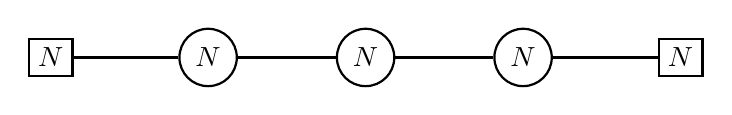
\begin{tikzpicture}[thick]
  \node[circle,draw] (one) at (0,0) {$N$};
  \node[circle,draw]  (two) at (2,0) {$N$};
  \node[circle,draw]  (three) at (4,0) {$N$};
  \node[rectangle,draw]  (flav1) at (-2,0) {$N$};
  \node[rectangle,draw]  (flav2) at (6,0) {$N$};
  \draw[-](one)--(two);
  \draw[-](two)--(three);
  \draw[-](one)--(flav1);
  \draw[-](flav2)--(three);
\end{tikzpicture}
\end{equation}
All the gauge couplings are exactly marginal since each gauge group has $2N$ flavours. The flavour symmetry of this theory is $\U(1)\times\U(1)\times\U(N)\times\U(N)$, where the $\U(1)$s come from the bifundamentals and the $\U(N)$s come from the fundamentals at the start and and of the quiver.\\
One can generate many more examples like this, for example
\begin{equation}
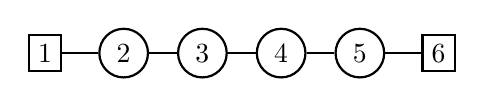
\begin{tikzpicture}[thick]
  \node[circle,draw] (one) at (0,0) {$2$};
  \node[circle,draw]  (two) at (1,0) {$3$};
  \node[circle,draw]  (three) at (2,0) {$4$};
  \node[circle,draw]  (four) at (3,0) {$5$};
  \node[rectangle,draw]  (flav1) at (-1,0) {$1$};
  \node[rectangle,draw]  (flav2) at (4,0) {$6$};
  \draw[-](one)--(two);
  \draw[-](two)--(three);
  \draw[-](three)--(four);
  \draw[-](one)--(flav1);
  \draw[-](flav2)--(four);
\end{tikzpicture}
\end{equation}
where, again, all the gauge couplings are marginal. One could ask why we do not branch around, but mathematically the shape of the graph is quite constrained by the requirement on the number of flavours. This is very similar to what happens with Dinkin diagrams in Lie algebras. The conformal quivers will always look like a sequence of gauge groups or that it bifurcates at the ends, or a loop (affine Dinkin diagrams). One can also get some exeptional diagrams.

One could also start to play with the gauge groups by looking at real groups: for $\USp(2N)$ we need $2N+2$ fundamentals so that the flavour group is $\SO(4N+4)$. The same can be said with an $\SO(2N)$ with $2N-2$ flavours. These allow to make quivers alternating $\USp$ and $\SO$ groups with half hypers connecting them. The continuous flavour symmetry will be just the one at the end of the quivers.

With a little bit of combinatorial work one can write down all the superconformal $\cN=2$ lagrangians with marginal couplings. What are the most general $\cN=2$ SCFT with gauge group $G=\SU(2)^{n}$? Let us write down some examples: 
\begin{enumerate}
	\item $\SU(2)$ with one adjoint is $\cN=4$ susy gauge theory. 
	\item $\SU(2)$ with $4$ fundamentals $N_{f}=4$, has $\SO(8)$ flavour symmetry.
\end{enumerate}
this is all with one gauge group. Let us go to two, beside trivial possibility of taking decoupled product of the last ones, 
\begin{equation}
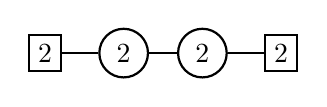
\begin{tikzpicture}[thick]
  \node[circle,draw] (one) at (0,0) {$2$};
  \node[circle,draw]  (two) at (1,0) {$2$};
  \node[rectangle,draw]  (flav1) at (-1,0) {$2$};
  \node[rectangle,draw]  (flav2) at (2,0) {$2$};
  \draw[-](one)--(two);
  \draw[-](one)--(flav1);
  \draw[-](flav2)--(two);
\end{tikzpicture}\qquad
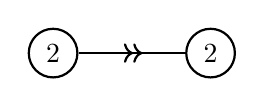
\begin{tikzpicture}[thick,decoration={
    markings,
    mark=at position 0.6 with {\arrow{>>}}}]
  \node[circle,draw] (one) at (0,0) {$2$};
  \node[circle,draw]  (two) at (2,0) {$2$};
  \draw[postaction={decorate}](one)--(two);
\end{tikzpicture}
\end{equation}
For the right one, one would think to have a $\U(2)$ flavour symmetry, but since the fundamental rep is pseudoreal, then the product of two fundamentals is real so we actually have a $\USp(4)$ flavour symmetry. The left one is more typical: there is a $\SO(4)^{2}$ coming from external fundamentals, while from the bifundamental there is a $\USp(2)$. But really the flavour group is $\SU(4)^{5}$ since $\SO(4)\sim\SU(2)\times\SU(2)$ and $\USp(2)\sim\SU(2)$.\\
Notice also that a pair of bifundamentals $(Q,\tilde Q)$ can be combined into one single $\hat Q$ which carries a $\USp(2)$ index
\begin{equation}
	\hat Q_{i_{1}i_{2}a}
\end{equation}
just writing $8=2\times2\times2$. These three indices play the same roles but the first two are gauged. But there is no reason to why I shouldn't be able to gauge other ones. We represent this object as a junction
\begin{equation}
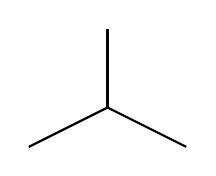
\begin{tikzpicture}[thick]
  \draw[-](0,0.5)--(0,-0.5);
  \draw[-](0,-0.5)--(-1,-1);
  \draw[-](0,-0.5)--(1,-1);
\end{tikzpicture}
\end{equation}
This adds two fundamental to every gauge group, but marginallity requires four fundamentals, and so we need two blocks, for example the $\SU(2)$ $N_{f}=4$ case is given by
\begin{equation}
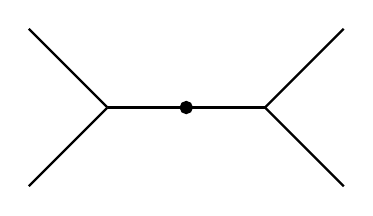
\begin{tikzpicture}[thick]
  \draw[-](0,0)--(1,-1);
  \draw[-](1,-1)--(0,-2);
  \draw[-](1,-1)--(2,-1);
  \draw[-](2,-1)--(3,-1);
  \draw[-](3,-1)--(4,0);
  \draw[-](3,-1)--(4,-2);
  \filldraw[black] (2,-1) circle (2pt) node[]{};
\end{tikzpicture}
\end{equation}
where the dot means the gauged group. We can also see, at least a subgroup, of the flabvour symmetry: in fact it is manifest an $\SU(2)^{4}\sim \SO(2)^{2}\subset \SO(8)$ flavour symmetry.

With this basic building block I can construct much more complicated theories. For any threevalent graph $\Gamma$ one gets a theory $T_{\Gamma}$ labelled by the graph. There are a couple of exeptional situations: take for example the following
\begin{equation}
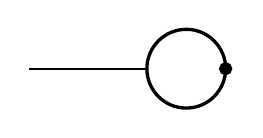
\begin{tikzpicture}[thick]
	\draw[-](0,0)--(1.5,0);
	\filldraw[color=black, fill=white, very thick](2,0) circle (0.5);
 	\filldraw[black] (2.5,0) circle (2pt) node[]{};
\end{tikzpicture}
\label{eq:N4}
\end{equation}
where two of the flavour symmetries are identified and gauged. What happens when we decompose $2\times 2\times 2a$? The first two give an adjoint plus a singlet that is not gauged. So this picture is $\SU(2)$ $\cN=$ plus a floating singlet. The singlet is important since now we can do 
\begin{equation}
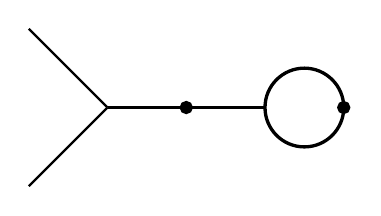
\begin{tikzpicture}[thick]
  \draw[-](0,0)--(1,-1);
  \draw[-](1,-1)--(0,-2);
  \draw[-](1,-1)--(2,-1);
  \draw[-](2,-1)--(3,-1);
  \filldraw[color=black, fill=white, very thick](3.5,-1) circle (0.5);
  \filldraw[black] (4,-1) circle (2pt) node[]{};
  \filldraw[black] (2,-1) circle (2pt) node[]{};
\end{tikzpicture}
\end{equation}
the adjoint, from the point of view of the central gauge group, looks like $3/2$ of a fundamental but with the singlet we have another $1/2$ fundamental that we can therefore gauge.

Let us discuss some of the properties of these theories $T_{\Gamma}$. Suppose to have $n$ external legs and $g$ loops. Without loops is very easy to count vertices and internal legs. Every loop removes two external legs and adds a vertex. Therefore we have $\SU(2)^{3g-3+n}$ gauge group. In particular there are going to be $3g-3+n$ gauge couplings $\tau_{i}$. There are also going to be $3g-3+n$ order parameters for the IR theory $\Tr\phi_{i}^{2}$ (coulomb branch order parameters).Notice that these order parameters and gauge couplings are intimately connected: if I want to change the gauge coupling I just take the lagrangian and add a prepotential term
\begin{equation}
	L+\delta\tau_{i}\int\dd[2]{\theta}\dd[4]{x}\Tr\phi^{2}_{i}
\end{equation}
There is also a flavour symmetry group $\SU(2)^{n}$, one for every external leg. In particular there are the mass parameters for this flavour group $\Tr M^{a}_{b}$. The mass parameter and the Coulomb branch scalars enter in the same way, so the mass parameters are just the order parameters for very weakly gauged flavour group.\\
For every $n,g$ the skeleton of the theory is the same, but they differ in how the matter couple.

\subsection{S-dualities}
We need to understand the S-dualities for these theories. We start from the simple cases. Consider $\cN=4$ $\SU(2)$ gauge theory. By moving in the Coulomb branch, the central charge $Z$ is uncorrected. The particles that move around in the Coulomb branch are: a W-boson (vector multiplet + hypermultiplet) which is half-BPS which has electric charge $1$ and magnetic charge $0$. At weak coupling it has a relatively small mass $Z=a$. Moving in the coulomb branch, we produce more particles. For example there is a magnetic monopole, half-BPS, and sit in the same multiplet as the $W$-boson but they have magnetic charge $1$ and electric charge $0$. It has a very heavy mass in the weak coupling limit $Z\sim \tau a$, but as $\tau\rightarrow 0$ they become lighter and lighter, becoming lighter than the $W$-boson. So in this limit, it does not make sense to think about the $W$-boson as the fundamental particle and as the monopole as some derived one. So we conjecture the existence of some sort of EM duality which exchanges them. The first test that this might be true, came out from looking at the full spectrum of magnetic monopoles and dyons. By quantizing one finds dyons $q_{M}=1$ and $q_{e}=n$. There are also magnetic monopoles with $q_{M}=2$ and dyons with $q_{e}=2n+1$. By going further one finds that there is a whole lattice of particles with electric and magnetic charges which are coprime $\gcd(q_{e},q_{m})=1$. By requiring that there is no wall crossing for half-BPS states, which means that the weakly coupled spectrum is actually the spectrum everywhere, we see that we have a spectrum of particles which is invariant under $\tau\rightarrow M\tau$ with $M\in \SL(2,\bbZ)$. This gives us a lot of weakly coupled regions which are divided by some strongly coupled regions.

One might wonder if the gauge coupling of the IR from which one can find the mass of the light fields, is the same parameter of the UV lagrangian. But this is an ill-defined question since the answer depends on the renormalization scheme. But we choose a renormalization scheme, when the masses are turned off, to have $\tau^{UV}=\tau^{IR}$.

Without wall crossing, we expect that the IR S-duality is still a symmetry in the UV since the spectrum of half-BPS states is the same.

Let us consider now the following theory $\SU(2)$ with $N_{f}=4$ flavours, which has $\SO(8)$ flavour symmetry. If the mass parameters, which sit in the cartan of $\SO(8)$, are turned off and if the vev of $\phi$ is zero, this theory has an exactly marginal gauge coupling $\tau$. By giving $\langle\Tr\phi^{2}\rangle=2a^{2}$ then, the central charge function cannot be corrected
\begin{equation}
	Z=(q_{e}+\tau^{IR}q_{m})a
\end{equation}
This theory seems to enjoy S-duality. But does the spectrum allow it? We have a $W$-boson ($q_{e}=2,q_{m}=0)$ plus a fundamental hypermultiplet which remember
\begin{equation}
	Q_{i}^{s}\tilde Q_{s}^{j}\phi^{i}_{j}
\end{equation}
becomes massless of mass $a$ and electric charge $1$. We have a flavour symmetry group which is unbroken so we label this particles by their $\SO(8)$ rep $\mathbf{8}_{v}$.\\
Surely there will be a classical solution in the Coulomb branch which is a smooth magnetic monopole solution with $q_{m}=1$ (quantizing it without flavour it is an hypermultiplet). With flavours there are more zero-modes: precisely there are $2N_{f}=8$ fermionic zero modes $\psi^{s}$ which transform in a vector of $\SO(8)$. What happens when we quantize them? We impose commutation relations
\begin{equation}
	\acomm{\psi^{s}}{\psi^{p}}=\delta^{sp}
\end{equation}
which tells us that these spinors are just gamma matrices that act on the monopoles: the monopole states live in spinor reps of the flavour group. Since the $\psi^{s}$ are also charged under the gauge group, they change the electric charge of the monopoles. The dyons
which have even electric charge sit in a positive chirality spinor and the ones with odd electric charge sit in a negative chirality spinor. There are also going to be particles with higher magnetic charges. Let us look just at the other ones for now.		
As $\tau\rightarrow\infty$ we are in the original weakly coupled limit, so we have a $W$-boson and hypermultiplet in $\mathbf{8}_{v,q_{e}}$. Then at $\tau=0$ we have monopoles in the spinor rep $\mathbf{8}_{s}$ while for $\tau=1$ we have ones in $\mathbf{8}_{c}$. This seems to be a problem but actually $\SO(8)$ has a $S_{3}$ outer automorphism group which exchanges these three representations\footnote{Symmetries of the Dynkin Diagram give rise to outer automorphisms of the Lie algebra. In the case where the Lie group is simply connected, such automorphisms are in one-to-one correspondance with group automorphisms. But when the Lie group is not simply connected all bets are off. Since $\pi_{1}(\SO(n))$ is of of order 2 (for $n>2$), some care must be taken. The second point is that the Dynkin Diagram of $\SO(8)$ actually has more symmetry, leading to the so called triality automorphism. This automorphism, in particular, maps $\text{Spin}(8)$, the universal covering, to itself and does not descend to $\SO(8)$.}. This is a good input by S-duality accompanied by the triality. In the fundamental region of the UHP we have three regions which are exchanged by the triality.

\subsubsection{Do the graph theory have S-dualities}
Let us start with the simplest theory $\SU(2)\times\SU(2)$

\begin{equation}
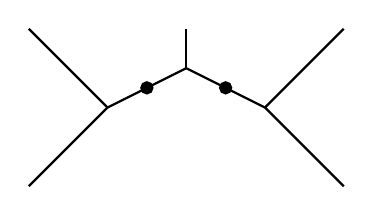
\begin{tikzpicture}[thick]
  \draw[-](0,0)--(1,-1);
  \draw[-](1,-1)--(0,-2);
  \draw[-](1,-1)--(2,-0.5);
  \draw[-](2,-0.5)--(2,0);
  \draw[-](2,-0.5)--(3,-1);
  \draw[-](3,-1)--(4,-2);
  \draw[-](3,-1)--(4,0);
  \filldraw[black] (1.5,-0.75) circle (2pt) node[]{};
  \filldraw[black] (2.5,-0.75) circle (2pt) node[]{};
\end{tikzpicture}
\end{equation}

All the fields are all fields with $3$ $\SU(2)$ indices some of which are gauge. The flavour symmetries are $\SO(4)\sim\SU(2)_{a}\times\SU(2)_{b}$ (from the left external legs) and an $\SU(2)_{c}$ (from the single internal leg) from the bifundamental and another $\SO(4)$ (from the other external legs). This theory hasd two exactly marginal gauge couplings $\tau_{1,2}$ and naively the parameter space should be the product of two upper half planes. I cannot go directly to IR but first explore the boundaries of this moduli space. I fix one gauge coupling to be very weak. In this region this theory just becomes $\SU(2)$ with $N_{f}=4$ with a very weakly gauged flavour symmetry group. This theory has three different lagrangian description. But if I want to see how this carries over to the original theory, I have to be careful to see what happens to the $\SU(2)$ flavour that I want to gauge and how the triality acts on it.\\
We have an $\SO(4)\times\SO(4)\subset\SO(8)$, therefore $\mathbf{8}_{v}=(\mathbf{4})\times(\mathbf{4})$. But the vector os $\SO(4)$ is just the product of the fundamental reps of the two $\SU(2)$ therefore becomes $(\mathbf{2}_{a}\times \mathbf{2}_{b})\times(\mathbf{2}_{c}\times \mathbf{2}_{2})$. Under triality, we excange $8_{v}$ with another $8_{s,c}$. The three cusps are just
\begin{equation}
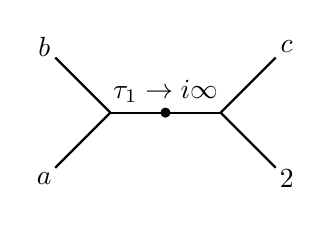
\begin{tikzpicture}[thick,scale=0.7]
  \node at (-.2,.2) {$b$};
  \node at (-.2,-2.2) {$a$};
  \node at (4.2,.2) {$c$};
  \node at (4.2,-2.2) {$2$};
  \draw[-](0,0)--(1,-1);
  \draw[-](1,-1)--(0,-2);
  \draw[-](1,-1)--(2,-1);
  \draw[-](2,-1)--(3,-1);
  \draw[-](3,-1)--(4,0);
  \draw[-](3,-1)--(4,-2);
  \filldraw[black] (2,-1) circle (2pt) node[above]{$\tau_{1}\rightarrow i \infty$};
\end{tikzpicture}\qquad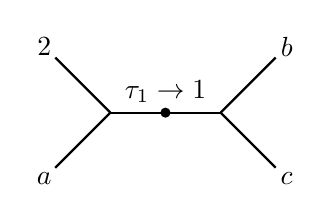
\begin{tikzpicture}[thick,scale=0.7]
  \node at (-.2,.2) {$2$};
  \node at (-.2,-2.2) {$a$};
  \node at (4.2,.2) {$b$};
  \node at (4.2,-2.2) {$c$};
  \draw[-](0,0)--(1,-1);
  \draw[-](1,-1)--(0,-2);
  \draw[-](1,-1)--(2,-1);
  \draw[-](2,-1)--(3,-1);
  \draw[-](3,-1)--(4,0);
  \draw[-](3,-1)--(4,-2);
  \filldraw[black] (2,-1) circle (2pt) node[above]{$\tau_{1}\rightarrow 1$};
\end{tikzpicture}\qquad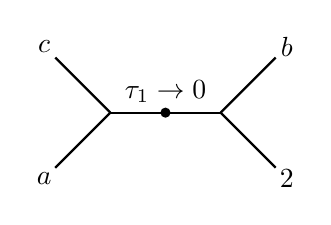
\begin{tikzpicture}[thick,scale=0.7]
  \node at (-.2,.2) {$c$};
  \node at (-.2,-2.2) {$a$};
  \node at (4.2,.2) {$b$};
  \node at (4.2,-2.2) {$2$};
  \draw[-](0,0)--(1,-1);
  \draw[-](1,-1)--(0,-2);
  \draw[-](1,-1)--(2,-1);
  \draw[-](2,-1)--(3,-1);
  \draw[-](3,-1)--(4,0);
  \draw[-](3,-1)--(4,-2);
  \filldraw[black] (2,-1) circle (2pt) node[above]{$\tau_{1}\rightarrow 0$};
\end{tikzpicture}
\end{equation}
which are exchanged by triality operation. So on the full theory, the triality acts as follows (where we can do the same job on the other coupling).

If the moduli space is really the product of two UHP we should be able to do S-duality on both nodes one after the other and viceversa and get the same result. 
\begin{figure}[H]
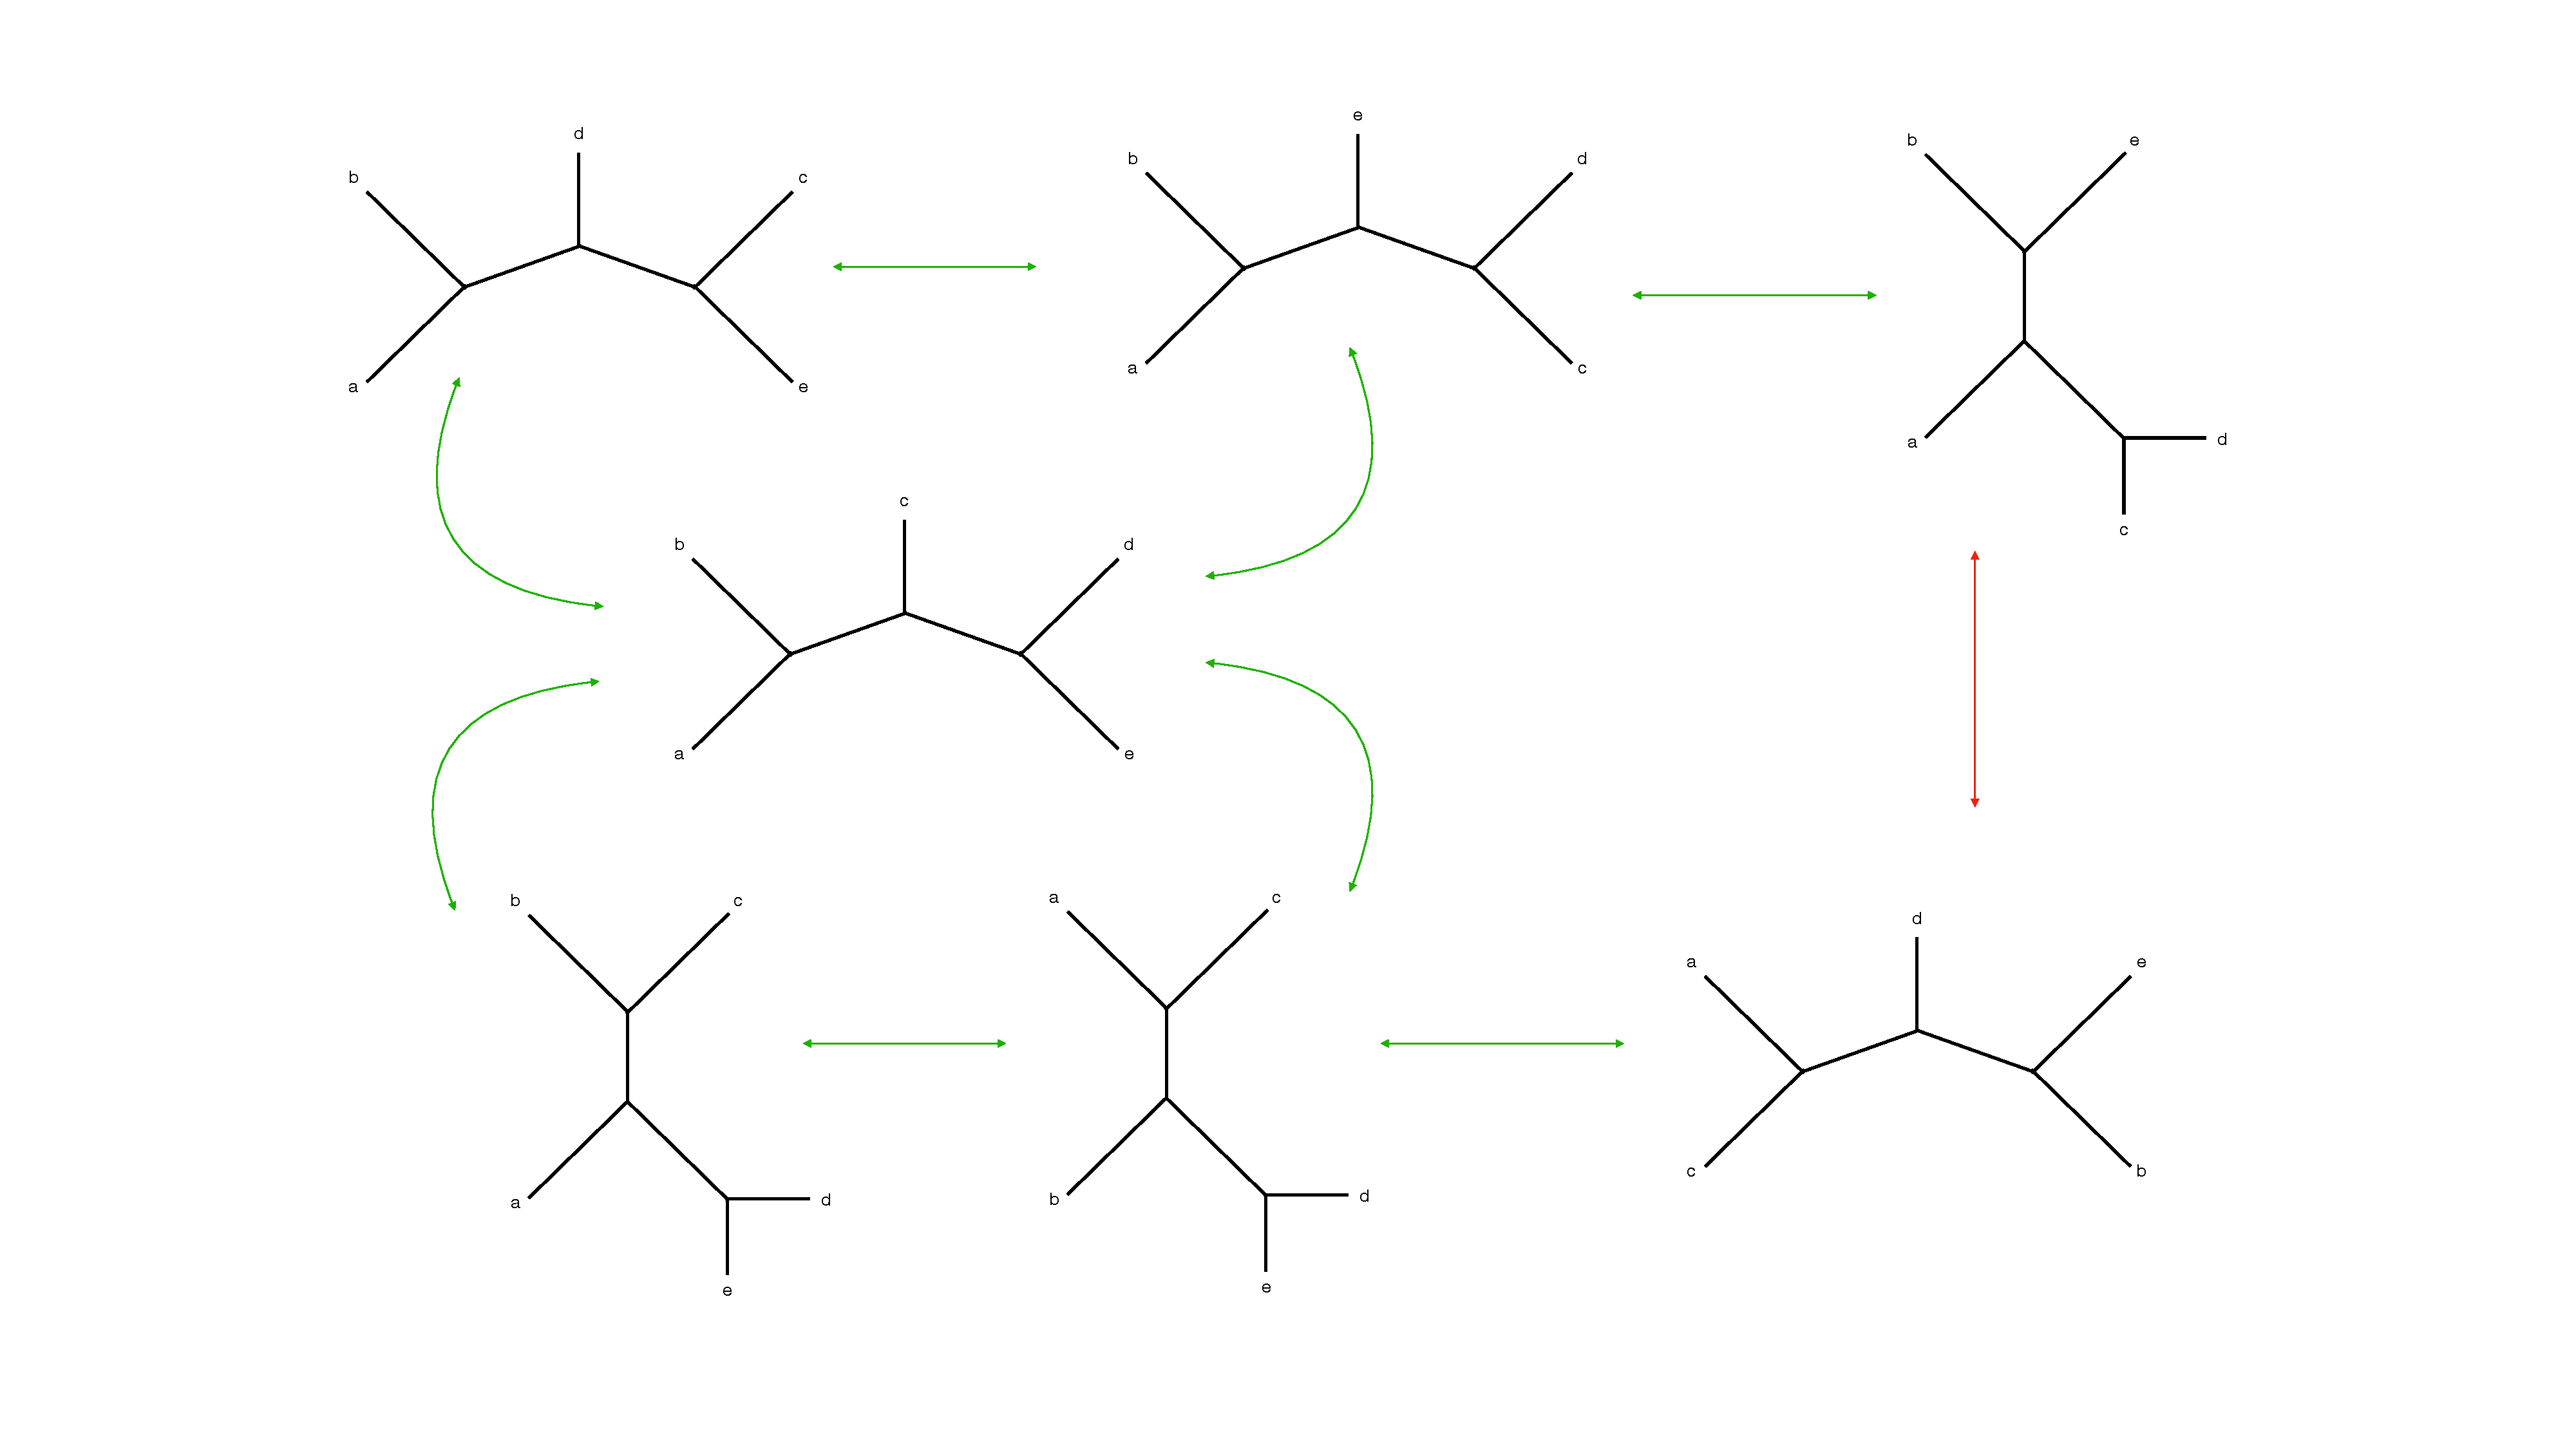
\includegraphics[width=\textwidth]{dualities.pdf}
\end{figure}
But what happens is that the two are not the same. But the two are related by S-duality. We found a pentagon of dualities. Here one gets a polytope made up of pentagons and triangles: the boundary of the parameter space (permutahedron, all the ways one can permute the $5$ flavour symmetries $5!/4$). So the hypotesis of the two UHP is wrong.

So what happens to a generic theory $T_{\Gamma}$? We have some trivalent graph and each S-duality operation reorganizes the four legs that come out of a segment. Through this basic operations we can relate all graphs with the same number of external leaves and loops (number of loops $g$ gives formula for dimension of Coulomb branch of the theory). There is a big moduli space $M_{g,n}$ (generalize notion of modular region?) of some $4d$ SCFT which with many cusps on the bundary each looking with some lagrangian description of $T_{\Gamma}$ with $g$ loops and $n$ leaves.\\
This $M_{g,n}$ has a bunch of charts in which I have a trivalent graph $\Gamma$ and a bunch of coordinates for each edge. Each chart looks like the upper region of the product of two UHP. But we want to combine all this charts together to glue the charts using S-dualities. This reminds us of Riemann surfaces. Instead of trying to build this $M_{g,n}$ by hand, I can see that there is a very famous moduli space with exactly the right dimension and properties. This is the space of complex structures of Riemann surfaces of genus $g$ with $n$ punctures. Let us see if we can really write charts which are naturally parametrized by the gauge couplings of my lagrangian.

Suppose to have a certain trivalent graph $\Gamma$. Associate to this graph a bunch of spheres with three marked points. We want to build out a Riemann surface of genus $g$ and $n$ punctures. There is a pretty natural way of doing it: every time I want to glue together two spheres to have a sensible Riemann surface which makes out my graph. What I can do is take some local coordinate system around this marked point and some local coordinates $z_{1}$ which goes to zero at the point. Take another one on the other sphere $z_{2}$ which goes together on the other marked point. To glue them together we declare that the following is satisfied
\begin{equation}
	z_{1}z_{2}=q
\end{equation}
where $q$ is some parameter. When $q=0$ we get the equation for two separate planes (so the two surfaces are disjoint and only touch at one point), with different $q$ they start merging together. So there is a certain patch in parameter space in the Riemann surface which has this coordinate system given by the $q_{i}$. To make sure is a good coordinate patch we should have $3g-3+n$ $q_{i}$s, and this number is the dimension of the moduli space of complex structures of the Riemann surface. As $q_{i}\rightarrow 0$ we get spheres which are connected together by very thin tubes.

We now claim that 
\begin{equation}
	q_{i}=e^{2\pi i\tau_{i}}
\end{equation}
so that the basic shift of the $\theta$ angle leaves the $q_{i}$ invariant. Now we need to see if it makes sense, especially for the S-duality transformation.

Take $\SU(2)$ with $N_{f}=4$. I can glue two spheres in two ways to get two patches in the moduli space of the theory
\begin{figure}[H]
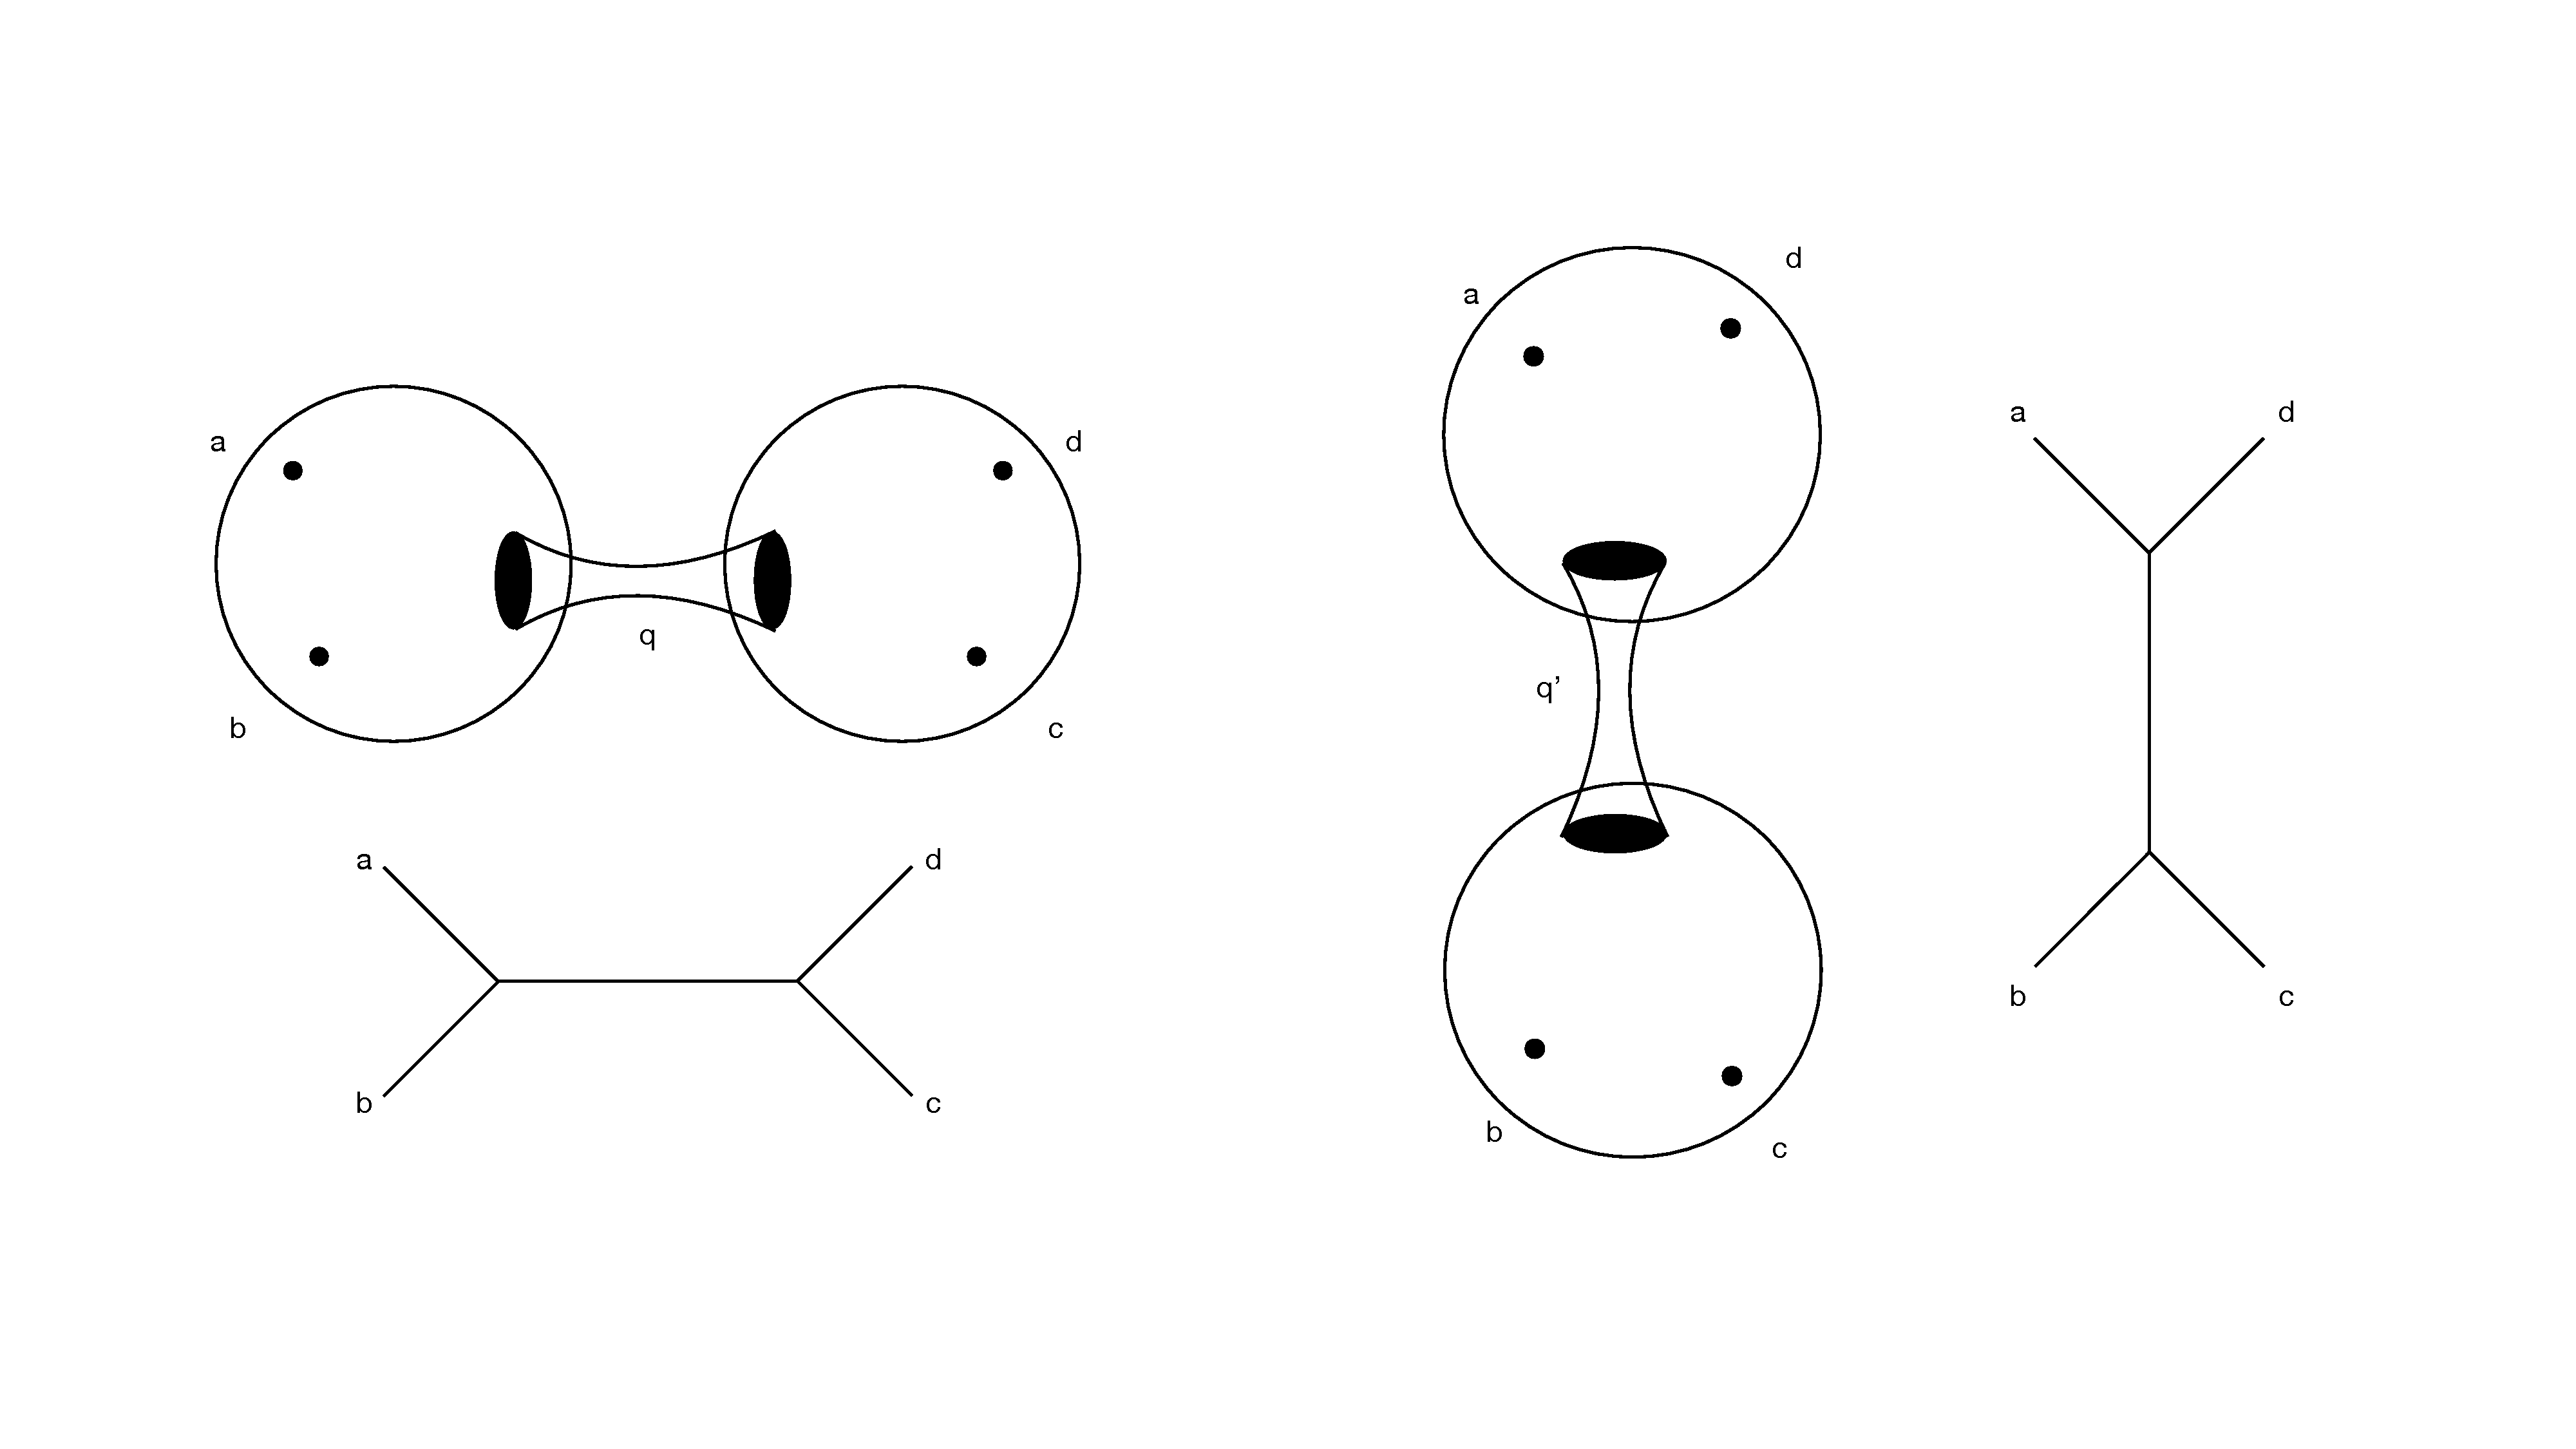
\includegraphics[width=\textwidth]{su2.pdf}
\end{figure}
The Riemann surface that we make with this gluing is just a sphere with four punctures. Suppose to put the puctures at $0,1,\infty$ where we picked some global coordinates on the spheres $z,w$ (Riemann sphere is $\bbC$). The gluing is just 
\begin{equation}
	\frac{z}{w}=q
\end{equation}
In the $w$ plane we have points at $0,1,q,\infty$. We wanted our parameter space to look like a UHP a (moduli space of the torus). Is very easy to make a torus out of a four punctured sphere: write the equation $y^{2}=P(z)$ where $P(z)$ is some polynomial with zeros at that four points
\begin{equation}
	y^{2}=z(z-1)(z-q)
\end{equation}
This describes an elliptic curve, a torus. The torus has a certain modular parameter $\tau(q)$. When comparing the three possibilities for the three theories one finds
\begin{equation}
	q\rightarrow1-q^{\prime},\qquad q\rightarrow\frac{1}{q^{\prime\prime}}
\end{equation}
and converting them to statements in $\tau$ they become exactly $\SL(2,\bbZ)$ transformations. The three patches really coincide with the three possible theories.

With this picture we can describe easily the moduli space. For example the (\ref{eq:N4}) graph, beign $\cN=4$ SYM is identified by taking the three-punctured sphere and connecting together two punctures $1,\infty$. In the $\bbC$ plane this looks like taking an annulus and connecting together the boundaries to make a torus. The modular parameter of the torus is then exactly the marginal coupling of $\cN=4$ SYM.

Now one would like to know that, now that we know the boundaries of the moduli space, there is going to be no problem going in. Since complex geometry is very strict we would expect it to work. To do so one should build the Seiberg-Witten curves and check that they really behave properly on the parameters (the IR lagrangian at each point).

So take above each point the Coulomb branch of the theory and check that it is fiberd properly and that it transforms well under S-dualities. Moreover the dimension of the CB is $3g-3+n$ which happens to be exactly as the dimension of the parameter space. This is not a coincidence: if you want to change the gauge coupling, you just need to change the lagrangian by adding a prepotential term
\begin{equation}
	L+\delta\tau_{i}\int \Tr\phi_{i}^{2}
\end{equation}
the expectation value of which is a coordinate on the CB $u_{i}$. Viceversa, every dimension two operator could be added to the lagrangian to give a coupling. So coupling and dimension two operators are in one-to-one correspondence. More is pretty clear that $u_{i}\delta\tau_{i}$ should be a 1-form, so should transform as a 1-form and this tells us how the CBs in each patches should be glued together. It should be glued together the same way as the cotangent bundle of $M_{g}$, $T^{*}M_{g}$. So the CB should be fiberd the same way as the cotangent bundle.

There is a very cute way to describe the cotangent bundle to a Riemann surface. First of all we should get a good way to describe $\tau_{i}$. How do I change the $q$s? I cut and then glue together again: take a path $\gamma$ and cut along the path and I glue it back after acting with a vector field which acts in a neighborhood of $\gamma$. Local transformation
\begin{equation}
	\delta\tau_{i}v^{i}\pdv{}{z}
\end{equation}
Quadratic differentials with single poles are just deformations in the coulomb branch. If one includes mass parameters on the punctures, the differential should have a double pole on the puncture.

\section{$q$-deformed YM}
This theory is relevant for the $2d-4d$ correspondence where a $6d$ theory is put on a product space $X_4\times C_2$ and compactified either on the first factor or on the second one. In the partition function of the $6d$ theory is a nice SUSY partition function that does not depende on the sizes of the two factors, then we expect the lower dimentional partition functions to match.\\
Such $2d$ theories are, for example, the Liouville-Toda theory or the $q$-deformed YM.
\subsection{$2d$ Yang-Mills}
In $2d$ there is no physical propagating degrees of freedom. Take $G$ to be a non-abelian Lie group. The action is of the form
\begin{equation}
	S\propto=\frac{1}{e^2}\int \dd[2]{x}\sqrt{\det g}\Tr F^2
\end{equation}
In $2d$ the only non-zero component of the curvature tensor is $F_{01}$ therefore
\begin{equation}
	\Tr F_{\mu\nu}F^{\mu\nu}=(g^{00}g^{11}-g^{01}g^{10})\Tr F_{01}^2=\det g^{-1}\Tr F_{01}^2
\end{equation}
so that 
\begin{equation}
	S \propto\frac{1}{e^2}\int\dd[2]{x}\sqrt{\det g}^{-1}\Tr F_{01}^2
\end{equation}
Therefore, the action only depends on the area of the surface, there is no additional dependence on the metric. This is a very special kind of $2d$ QFT. Whenever such a QFT is also a CFT, the theory is a $2d$ TQFT. The dependence on the coupling can be reabsorbed in the definition of the area.

We can solve this theory in many ways, but let us consider the Hamiltonian formalism putting the theory on cylinder. On $S^1$ we have an Hilbert space of states which, by taking the length of the circle to be $L$ can be defined as follows
\begin{equation}
	G\ni U=\text{Pexp}\int_0^L A_1 \dd x^1
\end{equation}
which is almost gauge invariant. At $0$ we still have a residual gauge transformation
\begin{equation}
	U\to gUg^-1
\end{equation}
So the Hilbert space is spanned by wavefunctions of $U$ which are invariant under the residual gauge transformation 
\begin{equation}
	\cH_{S^1}\ni \Psi(U)=\Psi(gUG^-1)
\end{equation}
One such basis for this Hilbert space is given by the characters of the representation $\chi_R(U)=\Tr_R U$ (class functions) which are indeed invariant under adjoint action. Moreover these are orthogonal given the following inner product
\begin{equation}
	\int \chi_R(U)\overline{\chi_{R^\prime}(U)}\dd{[U]}_{\text{Haar}}=\delta_{RR^\prime}
\end{equation}
Using the standard canonical quantization procedure, we can also find the Hamiltonian of the system. Being the only non-zero component of the curvature $F_{01}=E$, we have no magnetic field and therefore 
\begin{equation}
	H=\int_0^L\abs{E}^2\dd{x^1}=\int_0^L\frac{\delta}{\delta A_1(x_1)}\frac{\delta}{\delta A_1(x_1)}
\end{equation}
The action of the Hamiltonian on the basis is easily computed
\begin{equation}
\begin{split}
	H \chi_R(U) &= H \Tr_R\text{Pexp}\int_0^L T^a A_1^a\dd{x^1}\\
	&=\Tr_R\qty(\int_0^L T^a T^a) \dd{x^1}\Tr_R\text{Pexp}\int_0^L T^a A_1^a\dd{x^1}\\
	&=L c_2(R) \chi_R(U)
\end{split}
\end{equation}
which proves that the characters are indeed eigenstates of the hamiltonian. We can further idenfity the sides of the cylinder to get a torus $\bbT^2=S^1\times S^1$ and compute the partition function 
\begin{equation}
	Z_{2d}=\Tr_{\cH_{S^1}}e^{-HT}=\sum_R e^{-TL c_2(R)}
\end{equation}
which only depends on the area $TL$.

Next step, let us consider the following geometry: a disk with area $A$ (a sigar) where now
\begin{equation}
	\cH_{S^1}\ni \Psi_A(U)
\end{equation}
which we like to determine (Hartle-Hawking wavefunction). To determine it we can consider joining a cylinder with area $A^\prime$ to the cigar and get
\begin{equation}
	\Psi_{A+A^\prime}(U)=e^{-A H}\Psi_A(U)
\end{equation}
since we can easily change the area it is sufficient to know the zero area wavefunction. This can be understood from a path integral point of view. We have our spacetime to which there is cut out a zero-area disk. The holonomy around it needs to be one. Therefore the zero-area limit of this wavefunction must be a delta function. This is not square-integrable but we just add a constant
\begin{equation}
	\Psi_A(U)=\alpha\delta(U)=\sum_R f_R\chi_R(U)
\end{equation}
where the constants can be found as
\begin{equation}
	\alpha\chi_{R^\prime}(1)=f_{R^\prime}
\end{equation}
so that $f_R=\alpha \dim R$. Let us consider the pair of pants geometry with area $A$ so that we have three Hilbert spaces which should determine a vector in 
\begin{equation}
	\bigotimes_{i=1,2,3} H_{S^1}\ni \Psi_A(U_1,U_2,U_3)
\end{equation}
depending on the three holonomies.

By gluing a disk to one of the $S^1$ we get a cylinder with area $A+A^\prime$ to which we know the wavefunction. Therefore 
\begin{equation}
	\Psi_A(U_1,U_2,U_3)=\sum_R e^{-A c_2(R)}\frac{\chi_R(U_1)\chi_R(U_2)\chi_R(U_3)}{\dim R}
\end{equation}
We can now glue the three-punctured spheres in various ways to get many different geometries with different genus. For example, for genus $g=1$ with three punctures $n=3$ we can find 
\begin{equation}
	\frac{1}{\alpha^{2g-2+n}}\sum_R e^{-A c_2(R)}\frac{\prod_i \chi_R(U_i)}{(\dim R)^{2g-2+n}}
\end{equation}
Originally the constant $alpha$ came from the fact that the zero-area disk amplitude is a delta function which has to be normalized. On a genus $g$ surface, doing a QFT is very easy to generate a counterterm of the form 
\begin{equation}
	\delta S=\beta\int \dd[2]{x}\sqrt{g}R=\beta (2-2g)
\end{equation}
on a closed Riemann surface. This multiplies $Z$ by 
\begin{equation}
	e^{\beta(2-2g)}
\end{equation}
and the boundaries give some similar quantities depending on $n$. 

\subsection{$q$-deformed YM}
We consider the gauge group $G$ to be a standard Lie group. We deform it to a quantum group $G_q$ (the matrix entries become non-commutative). Take for example $\SU(2)_q$
\begin{equation}
	\begin{pmatrix}
		\alpha&\beta\\
		-\beta^*&\alpha^*
	\end{pmatrix},\qquad \alpha\beta=q\;\beta\alpha,\; \alpha\beta^*=q\;\beta^*\alpha,\ldots
\end{equation}
So we try to define a $2d$ YM in a lattice formulation for example, where all the link variables are replaced by a quantum group element instead of Lie group elements. This can be done in any dimensions but because of the non-commutativity one needs to define exacly in which order each link variable appears in the path integral. This is known at least in two dimensions how to do it consistently. In general dimensions is not known\dots

The end result is simple actually. Just replice the dimension of the rep by it's quantum dimension. When $G=\SU(N)_q$, then 
\begin{equation}
	\dim_q R = \chi_R\qty(\text{diag}(q^{\frac{N-1}{2}},q^{\frac{N-3}{2}},\cdots,q^{\frac{1-N}{2}})) 
\end{equation}
which in the limit $q\rightarrow1$ becomes $\chi_R(1)=\dim R$ as expected.

\subsection{Relation between Gaiotto theories and $q$-deformed YM}
Consider the superconformal index of $\cN=2$ $\SU(2)$ with $N_f=4$ flavours. This theory enjoys a special kind of S-duality discussed before. 

The relevant step in recongnizing the relationship between this theory and the $q$-deformed YM theory, is to consider the SCI of the Gaiotto theory in the limit of $q=t$. Consider in fact the half hypermultiplet contribution to the index 
\begin{equation}
	\Gamma(t^{1/2}z^\pm a^\pm b^\pm;p,q)\Gamma(t^{1/2}z^\pm c^\pm d^\pm;p,q)
\end{equation}
which explicitly, with $q=t$, gives
\begin{equation}
	\Gamma(t^{1/2}z^\pm;p,q)=\prod_{m,n\ge 0}\frac{1-z^{-1}p^{m+1}q^{n+\frac{1}{2}}}{1-zp^m q^{n+\frac{1}{2}}}\frac{1-z p^{m+1}q^{n+\frac{1}{2}}}{1-z^{-1}p^m q^{n+\frac{1}{2}}}
\end{equation}
There is a quasi complete cancellation between numerator and denominator such that the whole product just becomes
\begin{equation}
	\prod_{n\ge0}\frac{1}{1-q^{n+\frac{1}{2}}z}\frac{1}{1-q^{n+\frac{1}{2}}z^{-1}}
\end{equation}
and the dependence on $p$ vanished. This is due to the enanchement of SUSY in the aformentioned limit. 
\section{Localization}
\subsection{Equivariant cohomology}
We learn bosonic equivariant localization. Let $M$ be a compact orientable (this is needed for integration) manifold with some isometry group $G$. Equivariant cohomology is the genaralization of the cohomology of $M/G$ when this is not smooth. Choose $G=U(1)$. In this case even $G$ is compact, but is exists even for non-compact groups.\\
We take a metric on $M$, so is Riemmanian $(M,g)$ of even dimension $\dim M = 2l$. Since we have an isometry we have also a Killing vector $V=V^{\mu}\partial_{\mu}$ and the Lie derivative of the metric is zero $L_{V}g=0$ and the Killing equation also holds $\nabla_{(\mu}V_{\nu)}$. We have some common period $U(1)$ on $M$. We can consider forms in $M$, in particular the space of polyforms
\begin{equation}
	\bigwedge M = \left\{\alpha=\sum_{n=0}^{2l}\alpha_{n}|\alpha_{n}\in \bigwedge\nolimits^{n}M\right\}
\end{equation}
We can consider $V$-equivariant differntial $\ddv=d-\iota_{V}$ where
\begin{align}
	&d: \bigwedge\nolimits{n}M \rightarrow \bigwedge\nolimits^{n+1}M\\
	&\iota_{V}: \bigwedge\nolimits^{n} M \rightarrow \bigwedge\nolimits^{n-1} M
\end{align}
This object mixes object with different degree. We do not have grading now. But it can be taken back by putting a new parameter belonging to the algebra of $G$ which acts on $\iota_{V}$. The process of contraction does not require the metric.\\
We have that 
\begin{equation}
	\ddv^{2}= -\acomm{d}{\iota_{V}} = -L_{V}
\end{equation}
so we can restrict the space of polyform to the $V$-equivaiant polyforms
\begin{equation}
	\bigwedge{V}M= \left\{\alpha \in \bigwedge M | L_{V}\alpha=0\right\}.
\end{equation}
We do this so $\ddv^{2}$ is nihilpotent and we can define a cohomology.\\
The cohomology is defined as 
\begin{equation}
	H^{*}_{V}(M) = \frac{\ker \ddv|_{\Lambda_{V}M}}{\Im \ddv|_{\Lambda_{V}M}}
\end{equation}
This is called $V$-equivariant cohomology. If $M/G$ is smooth this cohomology reduces to the usual cohomology. If $G$ has fixed points this does not happen.\\
A form is equivariantly closed if $\ddv\alpha=0$ and equivariantly exact if $\alpha=\ddv\beta$ for some $\beta\in\Lambda_{V}M$.\\
The condition of equivariantly close mixes forms of different degrees. One can write the condition for every components, in particular of even and odd degree since they mix with each other but not between themselves.\\

We can now define integration on polyforms by integrating on the top form
\begin{equation}
	\int_{M}\alpha = \int_{M}\alpha_{2l}
\end{equation}
If we integrate an equivariantly exact form
\begin{equation}
	\int_{M}\ddv\beta = \int_{M}d\beta_{2l-1}=0
\end{equation}
when $M$ is compact. This is stokes theorem and applies also to equivariant polyforms. The integral depends only on the cohomology class
\begin{equation}
	\int_{M}(\alpha+\ddv\beta) = \int_{M}\alpha.
\end{equation}
We are interested of computing integrals of equivariantly closed forms. And the equivariant localization theorems tell us that this integrals only get contributions not from the whole manifold but only from the fixed points of the action on the manifold (Ahyia et al.).\\
If there are a finite number of points, this gives a finite sum of contributions to the integral. The neighbourhood of the fixed points
\begin{equation}
	M_{V}=\{ x\in M | V(x)=0\}
\end{equation}
is the only one that contributes.\\

Now some localization arguments: first argument use the Poincarè lemma. If we have a $V$-equivariant closed polyform on $M$ then this form is equivariantly exact not on full $M$, but just on $M\backslash M_{V}$. We can see this by construction. If we construct a $1$-form dual to the vector field (we need the metric now) $ \eta = g(V,\cdot) = g_{\mu\nu}V^{\mu}\mathrm{d}x^{\nu}$. This form is equivariant in the sense that $L_{V}\eta=0$ which is trivial.\\
We can compute its differential
\begin{equation}
	\ddv\eta = d\eta-\iota_{V}\eta = d\eta-|V|^{2}.
\end{equation} 
This differential is invertible in $M\backslash M_{V}$ (the manifold without the fixed points of $G$). Essentially
\begin{equation}
	(\ddv\eta)^{-1} = -\frac{1}{|V|^{2}}\left(1-\frac{d\eta}{|V|^{2}}\right)^{-1} = -\frac{1}{|V|^{2}}\sum_{n=0}^{l}\left(\frac{d\eta}{|V|^{2}}\right)^{n}
\end{equation}
from Taylor expansion. Obviusly with this definition
\begin{equation}
	(\ddv\eta)^{-1}\wedge \ddv\eta = 1.
\end{equation}
This form $(\ddv\eta)^{-1}$ is even equivariantly closed which can be checked from the invertibility condition.\\
We can define another polyform
\begin{equation}
	\Theta_{V}=\eta\wedge(\ddv\eta)^{-1}\qquad \ddv\Theta_{V}=1
\end{equation}
so that
\begin{equation}
	\alpha = \ddv(\Theta_{V}\alpha)
\end{equation}
on $M\backslash M_{V}$. Therefore $\alpha$ is exact. We only get contributions from the boundary of the space $M\backslash M_{V}$
\begin{equation}
	\int_{M}\alpha = \int_{\partial M\backslash M_{V}}\alpha.
\end{equation}
This does not tell us what the integral is, just says that the contribution comes from the fixed points of $G$ if the polyform is closed (the close condition is fundamental).\\
The second argument can say something on what the integral actually is. We have an equivariantly closed form $\alpha$ and we know that only the cohomology class counts for the integral. Therefore let us deform it 
\begin{equation}
	\alpha_{t} = \alpha\wedge e^{t \,\ddv \beta}
\end{equation}
where $\beta\in\Lambda_{V}M$, which means $L_{V}\beta=0$ so that $\alpha_{t}$ is also closed.\\
We can compute it
\begin{equation}
	\dv{t} \alpha_{t} = \alpha\wedge \ddv\beta e^{t\ddv \beta} = \ddv (\alpha\wedge \beta e^{t\ddv \beta})
\end{equation}
If we take $t=0$ we have the original integral. In particular consider $t\rightarrow\pm\infty$ and notice that the integral does not depend on $t$ as we have seen from the derivative since $\alpha$ is still closed. Choose $\beta=\eta$ defined before
\begin{align}
	\int_{M}\alpha = \lim_{t\rightarrow\infty}\int_{M}\underbrace{\alpha\wedge  e^{t\mathrm{d}\eta}}_{\text{polynomial in } t}e^{-t|V|^{2}}
\end{align}
The integrand is a polynomial of degree $l$ in $t$ which in fact we can expand. The other piece is a true exponential. When we take the limit, it gives us an exponential suppression that cannot be compensated by the polynomial in the limit. For any point for which $|V|^{2}\neq 0$ the exponential suppresses, just the points in the neighbourhood where $|V|^{2}$ is zero contribute. Which means that the integral localises on the fixed points of $V$.\\
We can use this expression to actually evaluate the integral. Let us assume that $V$ has only \textbf{isolated} fixed points. Since the integral localises on the fixed points, we can consider the expression only in a neighbourhood of the fixed points $P$ where the metric is essentially flat $\mathbb{R}^{2l}$
\begin{equation}
	\mathrm{d}s^{2} \simeq \sum_{i}^{l}(\mathrm{d}r_{i}^{2}+r_{i}^{2\mathrm{d}\phi^{2}})
\end{equation} 
which is just $l$ copies of $\mathbb{R}^{2}$. Each component of $V$ just does a rotation in the case of $G=U(1)$
\begin{equation}
	V\simeq\sum_{i=1}^{l}\omega_{P,i}\pdv{\phi_{i}}
\end{equation}
and also
\begin{equation}
	\eta\simeq \sum_{i=1}^{l}\omega_{P,i}r_{i}^{2}\mathrm{d}\phi_{i}
\end{equation}
where $\omega_{P,i}$ are the eigenvalues of the $G$ action on the tangent space around the point $P$.\\
Therefore
\begin{equation}
	\ddv \eta\simeq \sum_{i=1}^{l} (\omega_{P,i}\dd(r_{i}^{2})\wedge\dd\phi_{i}-\omega_{P,i}^{2}r_{i}^{2})
\end{equation}
and so we can actually evaluate the integral
\begin{align}
	\lim_{t\rightarrow\infty}\int_{N_{P}}\alpha\wedge e^{t\ddv \eta} = \lim_{t\rightarrow\infty}\prod_{i=1}^{l}\left[t\omega_{P,i}\int_{\mathbb{R}^{2}}\dd(r_{i}^{2})\dd{\phi_{i}}\alpha e^{-t\omega_{P,i}r_{i}}\right]
\end{align}
where we decomposed $\ddv\eta$ in two pieces, and we take only the leading contribution of the polynomial $t\omega_{P,i}$. Notice that the leading pice give us the maximal degree we can have on the manifold and so the only degree that contributes is the lower component. Around the point $\alpha$ is constant compared to the exponential suppression and so we can pick it out
\begin{equation}
	\lim_{t\rightarrow\infty} \alpha_{0}(P)\prod_{i=1}^{l}\left( t\omega_{P,i}\frac{2\pi}{t\omega_{P,i}^{2}}\right)=\alpha_{0}(P)\left(\frac{2\pi}{\prod_{i=1}^{l}\omega_{P,i}}\right)
\end{equation}
and we see that the powers of $t$ cancels out, as we wanted since it cannot depend on $t$ as we said. We get contributions only from the neighbourhood of the fixed points.\\
A more geometric, invariant, definition gives
\begin{equation}
	\alpha_{0}(P)\left(\frac{2\pi}{\text{Pf}(L_{V}(P))}\right).
\end{equation}
where $\text{Pf}$ is the Pfaffian of the invariant action of $G$ on the point $P$. The final formula is
\begin{equation}
	\int_{M}\alpha= (2\pi)^{l}\sum_{P\in M_{V}}\frac{\alpha_{0}(P)}{\text{Pf}(L_{V}(P))}
\end{equation}


Suppose we want to compute
\begin{equation}
	\int_{S^{2}}e^{ic\cos\theta}\dd\text{Vol}(S^{2})
\end{equation}
This can be done either with localization or with the usual techniques.

\subsection{Supersymmetry in curved space}
We want to apply this ideas to QFTs. So we start with the concept of Euclidean path integrals and some exact results.\\
One of the ideas is that when one has a QFT, all the information about it are in the path integral
\begin{equation}
	\int \mathcal{D} \phi e^{-S[\phi]/\hbar}
\end{equation}
but this object is too hard to compute. The standard paradigm is to evaluate them in a perturbative expansion, but this works only on small couplings. Even with resummation we still do not have all the informations coming from nonperturbative contributions.\\
We can choose some QFT where the path integral can be computed. We will be interested on theories on compact Euclidean manifolds $M$
\begin{equation}
	\mathcal{Z}_{M}(c) = \int\mathcal{D}\phi e^{-S[\phi,c]}
\end{equation}
as a function of some parameters $c$: parameters of the theory, of the manifold where we put the theory, parameters of the supersymmetric background chosen on the manifold (Festuccia-Seiberg etc). Why, if we are interested in Lorenzian spaces, we choose compact euclidean manifolds? The more phenomenological reason is that it is a profitable exercise to study SUSY QFTs on general compact manifolds and backgrounds
\begin{itemize}
	\item some manifolds and backgrounds are easier than others,\\
	\item different manifolds and backgrounds grant us access to different observables of a specific theory.
\end{itemize}
Very loosely we can distinguish three types of operators 
\begin{itemize}
	\item ``Order'' Operators: some functions of the fundamental fields which are in the lagrangian, local or non local. For example, in a $U(1)$ theory, we can have $F_{\mu\nu}(x)$ but of course we can consider non-local operators like Wilson lines 
	\begin{equation}
		W_{R}[\gamma] = \Tr_{R}P\exp{\oint_{\gamma} A}
	\end{equation}
	for some closed path $\gamma$ and rep $R$. This get computed directly in the path integral.
	\item ``Disorder'' operators: this are defined by removing some points from spacetime, either by removing a point for a local operator or a submanifold for a non-local operator, and then specify some boundary conditions around these points or submabifold, usually singular. To compute correlation functions for these operators we simply do
	\begin{equation}
		\langle \mathcal{O}_{D} \rangle = \int_{\text{B.C. choosen}}\mathcal{D}\phi e^{-S[\phi]}
 	\end{equation}
	We have like: 't Hooft line operators in $4d$ which are non-local, monopole operators in $3d$ which are local. The second ones are defined by removing a point and we remain with an $S^{2}$ around it and we impose that
	\begin{equation}
		\int_{S^{2}} F \in \text{ some conjugacy class}
	\end{equation}
	\item ``Defect'' Operators: again either local or non-local, points or submabifolds, where we introduce some extra fields that only live on the operator and not on the whole space. In this case we will need to integrate also on these localised degrees of freedom on some submanifolds $N\subset M$
	\begin{equation}
		\int \mathcal{D}\phi_{M}\mathcal{D}\phi_{N}e^{-S[\phi_{M}]}e^{-S_{N}[\phi_{N},\phi_{M}]}
	\end{equation}
	If we have for example a $1d$ curve in the manifold and we want to add some fermions on this line $\gamma$ then one can add 
	\begin{equation}
		S_{D} = \int_{\gamma}\dd\tau \bar{\psi}(\partial_{\tau}-iA_{\tau})\psi
	\end{equation}
	where $A_{\tau}$ are bulk fields pulled-back on the submanifold where the fermions live and are coupled to them.
\end{itemize}
All of these classes can be tackled with supersymmetric localization. 

Suppose we want to study a Wilson line for some gauge group $G$ in rep $R$. The same operator can be represented as some $1d$ defect operator in which we use the following action
\begin{equation}
	\mathcal{L}_{D} = \bar{\psi}(\partial_{\tau}-iA_{\tau}-i\tilde{A}_{\tau})\psi+i\tilde{A}_{\tau}
\end{equation}
where $\tilde{A}_{\tau}$ is a $U(1)$ gauge field, $A_{\tau}$ is the pull-back of the bulk gauge field and $\psi$ are fermions in rep $R$ under $A_{\mu}$ with charge $1$ under $\tilde{A}$.\\

The first step is to construct a susy theory on a curved manifold. Trivially we start in Lorentzian flat space with some susy theory with a susy algebra. In $4d$ minimal susy we have fermionic operators $\acomm{Q_{\alpha}}{\bar{Q}_{\beta}}=2\sigma^{\mu}_{\alpha\beta}P_{\mu}$. We also have susy currents $S_{\alpha\mu}$ that has the property that by integrating it we get the supercharges
\begin{equation}
	Q_{\alpha} = \int \dd[d-1]{x} S_{\alpha}^{0} \qquad \partial^{\mu}S_{\alpha\mu}=0
\end{equation}
A theory is supersymmetric if the lagrangian is invariant under susy transformations $\delta = \epsilon^{\alpha}Q_{\alpha}$ then $\delta\mathcal{L}=\partial^{\mu}(\cdots)_{\mu}$.\\
We go to euclidean $\mathbb{R}^{d}$ and we want to deform it to some manifold $M$ which is not flat. We want that a short distance the new theory gives the flat space theory. We only modify the theory in the infrared. We limit ourselves to relevant deformations to the flat space theory. Even with this prescription the construction is still ambiguous, the procedure is not unique. we call this ambiguity a background.\\
On top of this we want that the theory be supersymmetric: the supercharges preserved on the curved manifold will be a subset of the supercharges of the flat space. We have that the generators of the ``curved'' susy algebra $\subset$ flat space susy algebra. This new supercharges can be deformed such that in the limit we get the usual flat space algebra.\\
Is not always possible to preserve supersymmetry on any manifold. There will be some constraint on the geometry of $M$. When it is possible, we still have ambiguities.\\
One systematic approach to construct such simmetries is to couple the QFT to off-shell supergravity and then solving for the susy equations from the condition that come from the graviton multiplet of the sugra. In particular we set to zero the fermions, this guarantees that the variations of the bosons is zero and we insist that also the variation of the fermions, in particular the gravitino, is zero. This leads to the generalised Killing spinor equations
\begin{equation}
	\delta \psi_{\mu} = 2\nabla_{\mu}\epsilon + M_{\mu}(\substack{\text{SUGRA}\\\text{fields}})\epsilon=0
\end{equation}
In the sugra fields there are the metric, the other bosonic fields of the graviton multiplet etc. This equation is almost independent on the particular theory we put on the manifold. Still a given sugra can have different off-shell formulations since we can construct different supercurrent multiplets etc.\\
We have to solve this equation for $g_{\mu\nu}$, the other fields, $\epsilon$, which will give us how many supercharges are preserved on the given manifold.\\
Once we have a solution, we can plug it into sugra. This gives us two things
\begin{itemize}
	\item The deformed susy algebra
	\item The deformed matter action
\end{itemize}
When we go to Euclidean signature we have to complexify the fields and what might happen is that the background for this fields is not the analytic continuation of a real background in lorentzian signature. This means that we lose reflection positivity (euclidean version of unitarity). However what might happen is that the theory becomes superconformal in the infrared and some operators become redundant and the background fields that break reflection positivity couple to such operators and so they are not a problem.\\

Once we have the susy actrion on the curved manifold $S$ and a set of fermionic generators $Q$ such that $QS=0$, in general we have that $Q^{2}=\delta_{B}$ (bosonic symmetry). We are now interested in evaluating integrals of this form
\begin{equation}
	\mathcal{Z}_{M} = \int\mathcal{D}\phi e^{-S[\phi]}
\end{equation}
and in particular we want to evaluate a deformation of this integral by som $Q$-exact term
\begin{equation}
	\mathcal{Z}_{M}(t) = \int\mathcal{D}\phi e^{-S[\phi]-tQV[\phi]}
\end{equation}
where $\delta_{B}V=0$ which gives us an equivariant condition on the functionsl $V$. What is the dependence on this parameters
\begin{equation}
	\dv{t}\mathcal{Z}_{M}(t) = \int\mathcal{D}\phi\, QV e^{-S-tQV} = -\int\mathcal{D}\phi\, Q(Ve^{-S-tQV}) = 0
\end{equation}
Assuming that the measure is invariant under $Q$ (there are no anomalies, $\delta_{B}$ should be non anomalous) this is just a field redefinition and so the integral is zero. One has to be careful since we have infinite dimensional integrals since $Q$ acts as a total derivative on the supermanifold and the boundary terms can ruin the result. But since we have an exponential suppression we can make the naive argument still hold.\\
Suppose that this terms is not a deformation of the action, but is exactly one of the terms in the action which is $Q$-exact therefore we do not have a dependence from the couplings that come in front of $Q$-exact terms.\\
When we compute expectation values of the operators, they only depend on the $Q$ cohomology class of the operators. Moreover, the result shows that the path integral is not modified by this correction $QV$. This is exactly what we did before in the general theory of equivariant localization.\\
When we go to euclidean, by complexifying the fields we have that the dagger and the initial field become independent and so we have double the amount of fields, however we do not want to do the integral on all of them but only half of them in euclidean signature. We then have to choose a contour that takes half the fields and makes the integral convergent on all the values of $t$.\\

If we take $\mathcal{Z}_{M}(t=0)$ we get the original integral. Suppose we can find some $V$ such that the bosonic real part of $QV$ is positive semidefinite. Then we take the limit $t\rightarrow\infty$ then any configuration for which $QV$ is not zero is going to be infinitely suppressed, then only the configurations for which the real part of the bosonic part of $QV$ is zero is going to survive. The integral localizes around this configurations. Still we have to take into account the neighbourhood of the configuration. Let us expand around one of this points $\phi = \phi_{0}+t^{-1/2}\hat\phi$ ($\hat\phi$ parametrizes orthogonal directions) and 
\begin{equation}
	S+tQV = S[\phi_{0}]+(QV)^{(2)}_{\phi_{0}}[\hat\phi]+\order{t^{-1/2}}
\end{equation}
We need canonically normalized fields and this explains the $t$ factor in the deviation of $\phi$. We get a contribution from the field configuration onto which we localize plus a quadratic contribution that can be evaluated
\begin{equation}
	\int\mathcal{D}\phi_{0}\, e^{-S[\phi_{0}]}\frac{1}{\text{SDet'}((QV_{\phi_{0}})^{(2)})^{1/2}} 
\end{equation}
where the superdeterminant is just the ratio between bosonic and fermionic determinants. The prime is there for the zero modes that have to be removed by integrating over them. The integral over $\phi_{0}$ does exactly this. The fermionic zero modes, which are at the denominator, have to be reabsorbed either by some operators or by expanding the determinant.

What we have up to now is that localization tells us that the partition function localizes around field configurations for which the $Q$-exact correction is zero and does not exponentially suppress the integral.
\begin{equation}
	Z = \int_{\text{BPS}}\mathcal{D}\phi_{0}\,e^{-S[\phi_{0}]}\frac{1}{\text{SDet'}((QV_{\phi_{0}})^{(2)})^{1/2}}
\end{equation}
In good situations, the submanifold of the field configurations $\phi_{0}$ becomes one dimentional. The BPS stands for the locus of field configurations that satisfy the BPS equations. We have a canonical choice for $V$ which is
\begin{equation}
	V=\sum_{\text{fermions }\psi}(Q\psi)^{\dagger\dagger}\psi
\end{equation}
where the double $\dagger$ is there since, as we said, in euclidean signature complex conjugate fields become independent and this gives an anti-linear operator which does not have to be the same $\dagger$ as in lorentzian signature.\\
We need to check tha this $V$ satisfies the right constraint
\begin{equation}
	QV = \sum (Q\psi)^{\dagger\dagger}Q\psi+Q(Q\psi)^{\dagger\dagger}\psi
\end{equation}
where now we see that the zero locus of this is where $Q\psi=0$ which is the BPS equations.\\

\subsubsection{Examples}
We want to discuss a concrete example: $2d$ with $\mathcal{N}=(2,2)$ ($4$ supercharges) which is the dimensional reduction of $4d$ $\mathcal{N}=1$.\\
If we start in Lorentzian signature there are left and right moving spinors which are not related by charge conjugation and the biggest $R$-symmetry we can have is $U(1)\times U(1)\simeq U(1)_{V}\times U(1)_{A}$ where one acts on the right supercharges and one on the left supercharges. This is not part of the susy algebra in flat space, is an outer automorphism of the algebra, is required only when the theory is superconformal. But we will choose type of theories where the vector like $R$-symmetry is present. in general there can be two central charges, but if we have this $R$-symmetry we have only one central charge which is related to the broken part of the $R$-charge. We can have $1$ complex central charge.\\
If we go tu Euclidean the susy algebra looks like the following
\begin{align}
	\acomm{Q_{\alpha}}{\tilde{Q}_{\beta}} = [2\gamma^{\mu}P_{\mu}+2i\mathbb{P}_{+}Z+2i\mathbb{P}_{-}\tilde{Z}]_{\alpha\beta}
\end{align}
where the tilde is the independent complex conjugate, the $\mathbb{P}_{\pm}$ are chiral projectors, $Z$ and $\tilde{Z}$ are the complex central charge. The supercharges have $R$-charge $1$ for $Q$ and $-1$ for $\tilde{Q}$.\\

We want to put this theory on curved space: since we have these $R$-symmetry there exists an $R$ multiplet (which is the dimensional reduction of the $R$ multiplet in $4d$)
\begin{equation}
	R_{\mu} = (T_{\mu\nu},S_{\mu\alpha},\tilde{S}_{\mu\alpha},j^{R}_{\mu},j^{Z}_{\mu},j^{\tilde{Z}}_{\mu})
\end{equation}
plus we have a graviton multiplet
\begin{equation}
	G_{\mu} = (g_{\mu\nu},\psi_{\mu\alpha},\tilde{\psi}_{\mu\alpha},V_{\mu},C_{\mu},\tilde{C}_{\mu}).
\end{equation}
The latter obviously appear in covariant derivatives
\begin{equation}
	D_{\mu} = \nabla_{\mu} -irV_{\mu}+\frac{1}{2}z \tilde{C}_{\mu}-\frac{1}{2}\tilde{z}C_{\mu}
\end{equation}
plus they appear in field strength, that being 2-forms in two dimensions, we can use their dual scalars
\begin{equation}
	\mathcal{H} = i\epsilon^{\mu\nu}\partial_{\mu}C_{\nu}\qquad\tilde{\mathcal{H}} = -i\epsilon^{\mu\nu}\partial_{\mu}\tilde{C}_{\nu} 
\end{equation}
We should set to zero the variation of the fermions to zero (for the generalized Killing spinor equations)
\begin{align}
	&\frac{1}{2}\delta\psi_{\mu} = (\nabla_{\mu}-iV_{\mu})\epsilon - \frac{1}{2}\mqty(\mathcal{H}&0\\0&\tilde{\mathcal{H}})\gamma_{\mu}\epsilon+\cdots=0\\
	&\frac{1}{2}\delta\tilde{\psi}=(\nabla_{\mu}+iV_{\mu})\tilde\epsilon - \frac{1}{2}\mqty(\tilde{\mathcal{H}}&0\\0&\mathcal{H})\gamma_{\mu}\tilde\epsilon+\cdots=0
\end{align}
The dots appear in the full non-linear theory but when we set the variations to zero do not come up. In this equations we choose a basis in which the chirality is diagonalized.\\
Since we are in $2d$ the group of rotations is $SO(2)\simeq U(1)$ so that the bundle in which any field with spin trasforms is an abelian gauge bundle so there is no difference between spin and a standard abelian charge. This helps us do some semplifications: first the spin connection can be defined as
\begin{equation}
	\omega_{\mu}=-\frac{1}{2}\omega_{\mu}^{ab}\epsilon_{ab}
\end{equation}
so that the covariant derivative for spinors is just
\begin{equation}
	\nabla_{\mu}^{(s)} = \partial_{\mu}-is\omega_{\mu}
\end{equation}
which is just the standard abelian covariant derivative.\\
The deformed algebra will be given by the solution of the Killing spinor equations, setting $\delta_{\epsilon}=\epsilon^{\alpha}Q_{\alpha}$ we get
\begin{equation}
	\acomm{\delta_{\epsilon}}{\delta_{\tilde{\epsilon}}} = iL_{K}^{A}-i\epsilon \mathbb{Q} \tilde{\epsilon}
\end{equation}
where $L_{K}^{A}$ is a Lie derivative (translation) along a vector field which is specified by the spinors $K^{\mu} = \epsilon\gamma^{\mu}\tilde{\epsilon}$ and 
\begin{equation}
	\mathbb{Q} = \mqty(z-\sigma-\frac{r}{2}\mathcal{H} & 0 \\ 0 & \tilde{z}-\tilde{\sigma}-\frac{r}{2}\tilde{\mathcal{H}})
\end{equation}
and we have
\begin{equation}
	\acomm{\delta_{\epsilon_{1}}}{\delta_{\epsilon_{2}}} = 0.
\end{equation}
Now we can find the most general solutions to the Killing spinor equiations (Closset, Cremonesi 2014)
\begin{enumerate}
	\item On any orientable manifold we choose a vector field $V_{\mu}$ such that cancels the contribution to the spin connection in the covariant derivative $V_{\mu} = \frac{1}{2}\omega_{\mu}$ and set the scalar fields to zero $\mathcal{H}=\tilde{\mathcal{H}}=0$. For one of the two components of the spinor $\epsilon$ we cancel the contribution and the other is just constant 
	\begin{equation}
		\epsilon = \mqty(0 \\ \epsilon_{-}) \qquad \tilde{\epsilon} = \mqty(\tilde{\epsilon}_{+}\\0).
	\end{equation}
	This solution exists for any orientable manifold and is called \textbf{A-twist} and is a type of topological twist (just relate the $R$-symmetry to the spin connection). The algebra in this case is really simple $\delta_{\epsilon}^{2}=\delta_{\tilde{\epsilon}}^{2}=0$ and $\acomm{\delta_{\epsilon}}{\delta_{\tilde{\epsilon}}}=0$. For genus bigger than one this is the only possible solution.
	\item The \textbf{Untwisted} $\mathbf{S^{2}}$. We set $V_{\mu}=0$ and we turn on the scalar fields $\mathcal{H}=\tilde{\mathcal{H}}=i/R$ where $R$ is the radius of the sphere and the equations are of the form
	\begin{equation}
		\nabla_{\mu}\epsilon = \frac{i}{2R}\gamma_{\mu}\epsilon\qquad \nabla_{\mu}\tilde{\epsilon} = \frac{i}{2R}\gamma_{\mu}\tilde{\epsilon}
	\end{equation}
	which are known as conformal Killing spinor equations. We get two solutions for both, so in total there are four solutions. The topologically twisted solution is half BPS since it has only two solutions while this preserves all the supersymmetry. The deformed susy algebra has the following form
	\begin{equation}
		\acomm{\delta_{\epsilon}}{\delta_{\tilde{\epsilon}}} = iL_{K}-\frac{\epsilon\tilde{\epsilon}}{2R}R_{V}
	\end{equation}
	where we also have an $R$-symmetry rotation that disappears in the flat space limit. The $R$-symmetry became part of the algebra even thou at the start it was only an outer automorphism of the susy algebra, so we have to choose the $R$-charges. The Killing vector $K^{\mu}$ generates rotations of the sphere $SO(3)$. The full superalgebra is $SU(2)\times U(1)\subset SU(2|1)$ where the $U(1)$ is precisely the $R$-symmetry.
\end{enumerate}
We can now study localization of untwisted gauge theories on $S^{2}$ (round) in $2d$ $\mathcal{N}=(2,2)$ and we will restrict ourselves to vector and chiral multiplets
\begin{enumerate}
	\item Chiral multiplet $\Phi = (\phi,\psi,F)$ and the antichiral one.
	\item Vector multiplet $V_{\mu} = (A_{\mu},\sigma,\tilde{\sigma},\lambda,\tilde{\lambda}, D)$ where we can decompose $\sigma=\sigma_{1}-i\sigma_{2}$ and $\tilde{\sigma}=\sigma_{1}+i\sigma_{2}$. 
	\item Twisted chiral multiplet $\Sigma = (\sigma,\lambda_{+},\tilde{\lambda}_{-}, D-iF_{12}+i\tilde{\mathcal{H}}\sigma)$ and $\tilde{\Sigma} = (\tilde{\sigma},\lambda_{-},\tilde{\lambda}_{+},-D+iF_{12}-i\mathcal{H}\sigma)$.
\end{enumerate}
What is the data we can specify in this theory? 
\begin{enumerate}
	\item Gauge group $G$
	\item Matter representation $R$ of $G$. $\rho\in R$ are the weights of the representation $R$.
	\item Specify the $R$-charges since $SU(2|1)$ contains the vector-like $R$-symmetry.
	\item Interactions: superpotential $W(\Phi)$, twisted superpotential $W(\Sigma)$.
	\item Flavour symmetry $G_{F}$. This turns on some twisted masses $\langle \sigma^{F} \rangle$ which are just expectation values of the background flavour fields.
\end{enumerate}
We should construct now actions
\begin{equation}
\begin{split}
	\mathcal{L}_{\text{SYM}} &= \frac{1}{2g_{YM}^{2}}\Tr{\qty(F_{12}-\frac{\sigma_{2}}{R})^{2}+\qty(D_{\mu}\sigma_{1})^{2}-\comm{\sigma_{1}}{\sigma_{2}}^{2}+\qty(D_{\mu}\sigma_{2})^{2}+\qty(D-\frac{\sigma_{1}}{R})^{2}}\\
	&+\Tr{i\tilde{\lambda}\slashed{D}\lambda-i\tilde{\lambda}\comm{\sigma_{1}}{\lambda}+\tilde{\lambda}\gamma_{3}\comm{\sigma_{2}}{\lambda}}
\end{split}
\end{equation}
As it should, in the limit $R\rightarrow\infty$ we get back the flat space theory.
\begin{equation}
\begin{split}
	\mathcal{L}_{M} &= D_{\mu}\tilde{\phi}D^{\mu}\phi+\tilde{\phi}\qty[-iD+\sigma_{1}^{2}+\sigma_{2}^{2}+\frac{ir}{R}\sigma_{1}+\frac{2(2-r)}{4R^{2}}]\phi+F\tilde{F}\\
	&+i\tilde{\psi}\slashed{D}\psi+\tilde{\psi}\qty[-i\sigma_{1}+\sigma_{2}\gamma_{3}+\frac{r}{2R}]\psi+i\sqrt{2}\tilde{\psi}\tilde{\lambda}\phi+i\sqrt{2}\tilde{\phi}\lambda\psi
\end{split}
\end{equation}
If we want to perform localization we have to choose a contour, and the easier choice is a real contour: fields that where real in lorentzian signature are complexified in euclidean and we impose that they are real, when we have complex fields in euclidean we make them the complex conjugate of the other in lorentzian. In this choice the real part of the bosonic part of the action becomes positive definite and the integral is convergent.\\
The charges can be chosen as 
\begin{equation}
	\delta_{Q} = \delta_{\epsilon}+\delta_{\tilde{\epsilon}}
\end{equation}
Something nice happens: both the SYM action and the matter action are $Q$-exact.

\subsection{The $2d$ $\cN=(2,2)$ gauge theory}
We were studying the partition function of a $2d$ $\mathcal{N}=(2,2)$ gauge theories with vector and chiral multiplets on the untwisted round $S^{2}$ where we wrote the actions of the SYM part and the matter part
\begin{align}
	\mathcal{L}_{\text{SYM}} &= \frac{1}{2g_{YM}^{2}}\Tr{\qty(F_{12}-\frac{\sigma_{2}}{R})^{2}+\qty(D_{\mu}\sigma_{1})^{2}-\comm{\sigma_{1}}{\sigma_{2}}^{2}+\qty(D_{\mu}\sigma_{2})^{2}+\qty(D-\frac{\sigma_{1}}{R})^{2}}\\
	&+\Tr{i\tilde{\lambda}\slashed{D}\lambda-i\tilde{\lambda}\comm{\sigma_{1}}{\lambda}+\tilde{\lambda}\gamma_{3}\comm{\sigma_{2}}{\lambda}}\nonumber\\
	\mathcal{L}_{M} &= D_{\mu}\tilde{\phi}D^{\mu}\phi+\tilde{\phi}\qty[-iD+\sigma_{1}^{2}+\sigma_{2}^{2}+\frac{ir}{R}\sigma_{1}+\frac{2(2-r)}{4R^{2}}]\phi+F\tilde{F}\\
	&+i\tilde{\psi}\slashed{D}\psi+\tilde{\psi}\qty[-i\sigma_{1}+\sigma_{2}\gamma_{3}+\frac{r}{2R}]\psi+i\sqrt{2}\tilde{\psi}\tilde{\lambda}\phi+i\sqrt{2}\tilde{\phi}\lambda\psi\nonumber
\end{align}
which are $Q$-extact for the supercharge $\delta_{Q} = \delta_{\epsilon}+\delta_{\tilde{\epsilon}}$. The interactions of this theory are given by superpotential interactions as a holomorphic function of the chiral fields $W(\Phi)$. This function itself is a chiral multiplet and so as an $F$-term
\begin{equation}
	\mathcal{L}_{W} = i(F_{W}+\tilde{F}_{W}) = \delta_{Q}(\cdots) \qquad F_{W}=\partial_{i}WF_{i}+\frac{i}{2}\partial_{ij}^{2}W \psi_{i}\psi_{j}
\end{equation}
which is also $Q$-extact. We also have the twisted superpotential $W(\Sigma)$ where we restrict to the case where this is linear
\begin{equation}
	W = \frac{i}{2}\qty(\xi+i\frac{\theta}{2\pi})\Tr\Sigma \rightarrow \mathcal{L}_{FI} = \Tr{i\xi+i\frac{\theta}{2\pi}F_{12}}
\end{equation}
which is not $Q$-extact and so the partition function will depend on it. Finally we have twisted masses related to flavour symmetrys (they take value in the Cartan of the flavour symmetry) and are associated to the central charge of the susy algebra. In order to have the theory supersymmetric we have to impose
\begin{equation}
	\delta\lambda^{\text{flav}} = 0.
\end{equation}
Given that the given terms are $Q$-exact we could use them to do localization with the said real contour so that the two terms have positive real parts. The matter term is positive as long as $0<r<2$. We localize on the zero part of that lagrangians, which for the matter part is  (BPS configurations)
\begin{equation}
	F_{12}=\frac{\sigma_{2}}{R},\quad D = \frac{\sigma_{1}}{R},\quad D_{\mu}\sigma_{1}=D_{\mu}\sigma_{2}=\comm{\sigma_{1}}{\sigma_{2}},\quad \phi=\tilde{\phi}=F=\tilde{F}=0
\end{equation}
which is a very simple zero loci. This easily parametrizes the moduli space
\begin{equation}
	D = \frac{a}{R^{2}},\quad F_{12}=\frac{m}{2R^{2}}
\end{equation}
plus a GNO quantization condition on the field strength
\begin{equation}
	\frac{1}{2\pi} = \int_{S^{2}}F_{12}=2\implies e^{2\pi i m}\in\mathbb{1}_{G}
\end{equation}
so $m$ is quantized. The classical action is just given by the only non $Q$-exact term which is the twisted superpotential
\begin{equation}
	S^{(0)}_{FI} = 4\pi i \xi \Tr \sigma_{1}+i\theta \Tr m
\end{equation}
and the one loop determinant has to be computed. By working off-shell we can compute for different multiplets the contributions to the determinant. In general is a very difficult problem to compute the full spectrum of the theory to find the determinant, but in this case, which is very symmetric, is doable. We decompose the fields which are into the line bundle into harmonics (sphere spherical harmonics) 
\begin{equation}
	Y^{s}_{j,j_{3}}\qquad j,j_{3}\in \mathbb{Z}+s, |j_{3}|,|s|\le j, s=s_{z}-\frac{m}{2}
\end{equation}
which are just the eigenfunctions of the laplacian
\begin{equation}
	R^{2}D_{\mu}D^{\mu}Y^{s}_{j,j_{3}} = \qty[-j(j+1)+s^{2}]Y^{s}_{j,j_{3}}
\end{equation}
For the chiral multiplet we get by expanding the action up to second order and plugging in the zero modes
\begin{equation}
	\mathcal{O}_{\phi} = -D_{\mu}D^{\mu}-iD+\sigma_{1}^{2}+\sigma_{2}^{2}+\frac{ir\sigma_{1}}{R} +\frac{r(2-r)}{4R^{2}}
\end{equation}
which gives, by using the harmonic expansion
\begin{equation}
	\det \mathcal{O}_{\phi} = \prod_{j=\frac{|m|}{2}}^{\infty}\qty(j+\frac{r}{2}-ia)^{2j+1}\qty(j+1-\frac{r}{2}+ia)^{2j+1}
\end{equation}
The same goes for the fermionic part
\begin{equation}
	\mathcal{O}_{\psi} = \cdots + \mqty(Y^{\frac{1}{2}-\frac{m}{2}}_{j,j_{3}} \\  Y^{-\frac{1}{2}-\frac{m}{2}}_{j,j_{3}} )
\end{equation}
which gives
\begin{equation}
	\det\mathcal{O}_{\psi} = (-1)^{\frac{m+|m|}{2}}\prod_{j=\frac{|m|}{2}}^{\infty}\qty(j+\frac{r}{2}-ia)^{2j}\qty(j+1-\frac{r}{2}+ia)^{2j+2}
\end{equation}
As we can see, like we said before, some contributions cancel in the ratio of the two determinants
\begin{equation}
	\frac{\det\mathcal{O}_{\psi}}{\det\mathcal{O}_{\phi}} = \prod_{n=0}^{\infty}\frac{n+1-\frac{r}{2}+ia-\frac{m}{2}}{n+\frac{r}{2}-ia-\frac{r}{2}}
\end{equation}
but this expression needs to be regularized. We can use the zeta function regularization
\begin{equation}
	\zeta(z,q) = \sum_{n=0}^{\infty}(q+n)^{-z}
\end{equation}
and taking
\begin{equation}
	-\pdv{z}\zeta(z,q)\eval_{z=0} = \log\prod_{n=0}^{\infty}(q+n) = \log\frac{\sqrt{2\pi}}{\Gamma(q)}
\end{equation}
and so
\begin{equation}
	Z_{1-\text{loop}}^{\text{chiral}} = \prod_{\rho\in R}\frac{\Gamma\qty(\frac{r}{2}-i\rho(a)-\frac{\rho(m)}{2})}{\Gamma\qty(1-\frac{r}{2}+i\rho(a)-\frac{\rho(m)}{2})}
\end{equation}
We want to do something similar for the vector multiplet but first we need to fix the gauge by using the standard Faddeev-Popov method. However, we are expanding around a certain configuration and so we have to do gauge fixing on a background, not around the zero configuration, and what we do is
\begin{equation}
	A_{\mu} = A_{\mu}^{(0)}+\frac{1}{\sqrt{z}}\hat{A}_{\mu}
\end{equation}
and we do gauge fixing on the oscillations
\begin{equation}
	\mathcal{L}_{GF} = -\tilde{c}\qty(D^{\mu}D_{\mu}c-iD^{\mu}\comm{\hat{A}_{\mu}}{c})-\frac{1}{2\xi_{GF}}(D^{\mu}\hat{A}_{\mu})^{2}
\end{equation}
We can use now SYM+GF which is quadratic, and the one loop determinant will have a similar form
\begin{equation}
	\frac{\det\mathcal{O}^{\prime}_{c}\det\mathcal{O}_{\lambda}}{\sqrt{\det\mathcal{O}^{\prime}_{A,\sigma}}} = \prod_{\alpha(m)=0}\frac{1}{|\alpha(a)|}\prod_{\alpha>0}(-1)^{\alpha(m)}\qty(\frac{\alpha(m)^{2}}{4}+\alpha(a)^{2})
\end{equation}
where we have to remove the zero modes that are present even in ghosts since we are on a compact space and we cannot set to zero the constant solutions. The $\alpha(m)=0$ are the roots that are invariant under the magnetic flux $m$. The zero modes of the denominator span the Cartan subalgebra which commutes with the magnetic flux. We should integrate over the zero modes
\begin{equation}
	\frac{1}{|W_{m}|}\int \prod_{n=1}^{\rank G}\frac{\dd{a_{n}}}{2\pi}\prod_{\alpha(m)=0}|\alpha(a)|\sum_{m\in\Gamma_{mag}}\frac{1}{|W \backslash W_{m}|}
\end{equation}
where $W_{m}$ is the Weil group that leaves the magnetic flux invariant.\\
When we put everything together we get the following expression
\begin{equation}
\begin{split}
	Z_{S^{2}} &= \frac{1}{|W|}\sum_{m\in\Gamma_{mag}}\;\int\limits_{\mathbb{R}^{\rank G}}\prod_{n=1}^{\rank G}\frac{\dd a_{n}}{2\pi}e^{-4\pi i\xi\Tr a-i\theta \Tr m}\\
	&\times\prod_{\alpha>0}(-1)^{\alpha(m)}\qty(\frac{\alpha(m)^{2}}{4}+\alpha(a)^{2})\prod_{\rho\in R}\frac{\Gamma\qty(\frac{r}{2}-i\rho(a)-\frac{\rho(m)}{2})}{\Gamma\qty(1-\frac{r}{2}+i\rho(a)-\frac{\rho(m)}{2})}
\end{split}
\end{equation}
Here all the twisted masses are zero. But can be easily found since the come on the same footing of $a$ although being non-dynamica. A few comments
\begin{enumerate}
	\item It is a relatively simple expression
	\item It is an exact non-perturbative result, in particular it should contain all instanton corrections which are not manifest from the result. One way to see them is to consider the $\rank G=1$ case where the integral is on the real line. To do this integral one can use the Cauchy integral formula closing the contour in the upper half plane which reduces to a sum of residues and what one discovers is that there is a $\rank $ $2$ wedge coming from the sum on the magnetic lattice and all of this residues come from instanton contributions.
	\item One might be interested now in operator insertions to compute expectation values. For example one can insert twisted chiral fields on one point of the sphere and anti-twisted chiral fields at the antipodal point of the other one. In this case we do not have an holomorphic operator which cannot be found by topological twists. It is also easy to add Wilson lines on the sphere. In this case the expectation values of such operators are given by simply adding such operators in the found result.
	\item If one studies $3d$ $\mathcal{N}=2$ gauge theory on $S^{3}$ the result is very similar.
	\item If one studies $4d$ on $S^{4}$ one needs to evaluate separately the instanton corrections.
	\item This integral does not depend on the RG flow. An interesting setup is to start from a Gauged Linear Sigma Model for which we know the exact result of the partition function and then flow in the IR to a conformal Non Linear Sigma Model and infer result on this IR theory. 
\end{enumerate}
But how does this expression know about instantons? What if one chooses a different localization term: suppose to add another one to the ones used up to now
\begin{equation}
	\mathcal{L}_{H} = \Tr\qty[-i\qty(D-\frac{\sigma_{1}}{R})(\phi\tilde{\phi}-\chi)+\cdots] = \delta_{Q}(\cdots)
\end{equation}
where $\chi$ is a constant. Notice that this added term looks like a FI term dressed with other stuff in such a way that there is no dependence on it. While this action is not manifestly positive semidefinite, however $D$ appears in the action without derivatives and quadratically. Therefore one can do the integral on $D$ and we get back a positive definite term. We therefore substitute the F-terms for $D$ and get 
\begin{equation}
	D-\frac{\sigma_{1}}{R}=i(\phi\tilde{\phi}-\chi)
\end{equation}
which looks like a $D$-term equation but with a FI term. The nice thing is that in $2d$ when turning on a FI term, the vacua get move to the Higgs branch and on the Higgs branch there are vortices. One might expect that the zero locus might move to something that looks like the Higgs branch in flat space and so the configurations that matter are vortices. Before what we had looked like a Coulomb branch.\\
By imposing the constraint and solving the BPS equations we get
\begin{equation}
	(\sigma_{1}-M)\phi = \sigma_{2}\phi=0
\end{equation}
where $M$ are twisted masses, $\sigma_{1}$ is a diagonal matrix in $\mathfrak{g}$. Moreover one finds some differential equations that depend on $\chi$ but since there is no real dependence on $\chi$ one can take it to infinity and study them there
\begin{figure}[H]
\centering
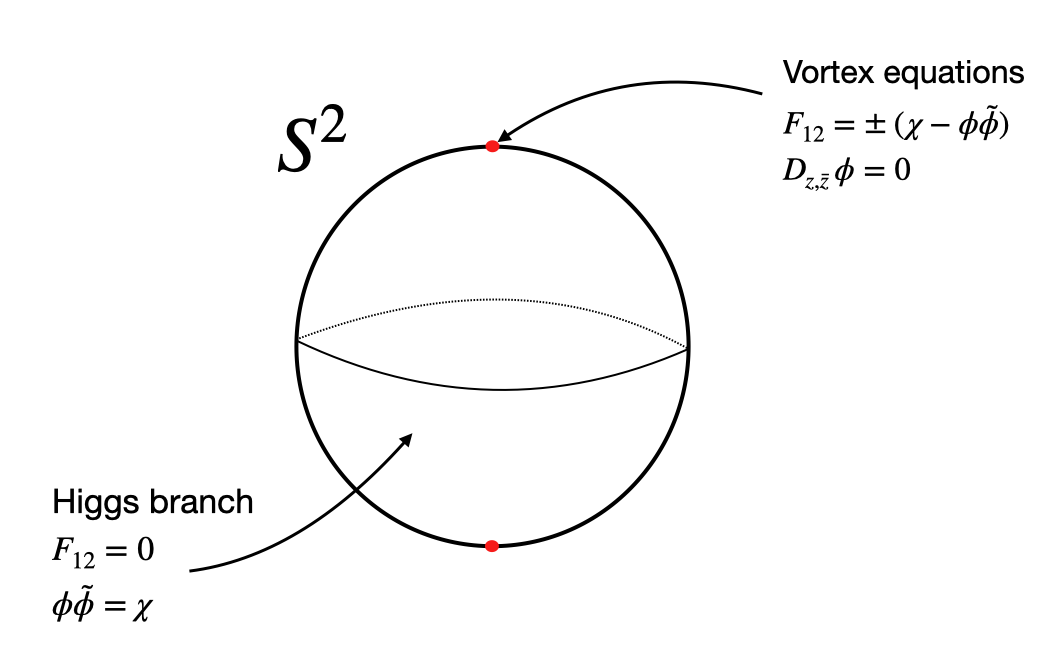
\includegraphics[width=.7\textwidth]{sol.png}
\end{figure}
The solution to the vortex equations are known to be instantons in $2d$. And now when we localize we have a finite sum on the Higgs branches. 

\subsection{Higgs branch localization}
New we will study what is called Higgs Branch Localization. Before we added a new $Q$-exact term that was not positive definite but by using $D$-term equations we could make it positive definite which was like changing the integration contour. We had two different solutions for the BSP equations on the sphere in the limit
\begin{equation}
	\underset{Q-\text{exact}}{\chi}\rightarrow\infty
\end{equation}
which is a ``fake'' parameter. \\
The moduli space of solutions of the vortex equations is separated into disconnected branches and each branch is characterized by a number: the vortex (or instanton) number. If we take $U(N)$ for example 
\begin{equation}
	k = \frac{1}{2\pi}\int_{\mathbb{R}^{2}}F \in \mathbb{Z}
\end{equation}
So the final form of the formula will be
\begin{equation}
\begin{split}
	\mathcal{Z}_{S^{2}} = \sum_{\substack{\text{Higgs}\\ \text{Branch}\\ \text{(Finite)}}}e^{S_{cl}}\mathcal{Z}^{\prime}_{1-\text{loop}}\mathcal{Z}_{\text{vortex}}(q)Z_{\overline{\text{vortex}}}(\overline{q})
\end{split}
\end{equation}
where the $1$-loop determinant is similar to the last one. The interesting part are the other pieces: the vortex part comes out to be like the one for a theory in an $\Omega$-background since the poles are not flat, there is some residual curvature. This theory gives us a background potential which traps the vortices in the origin which makes the moduli space somewhat compact since the vortices cannot move to infinity
\begin{equation}
	\mathcal{Z}_{\text{vortex}}(q) = \sum_{k\ge 0}q^{k}\int_{\mathcal{M}_{k,\text{vortex}}}\dd{\text{Vol}}_{equiv},\qquad q=e^{-4\pi\xi-i\theta}
\end{equation}
What about the $\mathcal{M}_{k,vortex}$ moduli space? It is Kähaler and symplectic. In particular there is a closed symplectic $2$-form $\omega$ which gives us the volume through the $\mathrm{d}\omega$. In particular $\dd{\text{Vol}} = \omega^{l}/l!$ which in particular is infinite. In fact we want to evaluate the equivariant volume. First of all we have rotations of $\mathbb{R}^{2}$ and moreover we have flavour rotations of $\phi$. The first is abelian, in the second we take the maximal torus (we do equivariant cohomology on the maximal torus). For each of this we have to introduce a vector field $V$ (which is very general for now). The volume form is equivariant under the action of $V$ ${L}_{V} \omega=0$ however is not equivatiantly closed. We construct the equivatiantly closed form $\dd{\text{Vol}} = \exp\qty(\omega+\mu)$ where $\mu$ is the moment map for the $U(1)^{\#}$ action where $\dd{\mu} = \iota_{V}\omega$. One can show that this is equivatiantly closed.\\
What we would like to compute is (using a physicist way)
\begin{equation}
	\int_{\mathcal{M}_{k,\text{vortex}}}\dd{\text{Vol}}_{equiv} = 0d \text{ path integral of a theory that has } \mathcal{M}_{k,vortex} \text{ as its moduli space}
\end{equation}
This is called ADHM construction. The point is finding what this theory is. Let us consider a specific example: $2d$ $\mathcal{N}=(2,2)$ $U(N)$ SQCD with $N_{f}$ fundamentals and $\tilde{N}_{f}$ antifundamental with $N_{f},\tilde{N}_{f}>N$ and a FI $\xi>0$. We want to understand the vortex moduli space of this theory which was done by Hanany and Tong in 2003. We go to the $k$-vortex sector which is a $0d$ theory (dimensional reduction of $2d$ $\mathcal{N}=(0,2)$ which has the following ingredients: $U(k)$ vector $(\phi,\lambda,\bar{\lambda},D)$, one adjoint chiral $X,\chi$, $N$ fundamental chirals $I,\mu$, $N_{f}-N$ antifundamental chirals $J,\nu$ and $\tilde{N}_{f}$ fundamental Fermi multiplet $\xi, G$ (fermion and auxiliary scalar). To compute the equivariant volume we have to do the path integral of this theory which is a matrix model and is simple. Again we can use localization on this theory which is much more simple than the initial integral.\\
Essentially we have to compute the $1$-loop determinants
\begin{equation}
	\text{Chiral}\longrightarrow\int\dd{X}\dd{X}^{\dagger}\dd{\chi}\dd{\chi}^{\dagger}e^{-X^{\dagger}\phi^{2}X-\chi^{\dagger}\phi\chi}\sim \frac{1}{\phi}
\end{equation}
which by the example we can see that they are very easy. The result at the end is
\begin{equation}
	\mathcal{Z}_{k}=\oint_{C}\prod_{I=1}^{k}\frac{\dd{\phi}_{I}}{2\pi i} \mathcal{Z}_{vec}(\phi)\mathcal{Z}_{chiral}(M,\phi)\mathcal{Z}_{fermi}(\tilde{M},\phi)
\end{equation}
the contour is called Jeffry-Kirwan residue. By computing this residues 
\begin{equation}
	\mathcal{Z}_{vortex}^{SQCD} = \sum_{\vec{k}}\frac{q^{\abs{\vec{k}}}}{\vec{k}!}\frac{\prod_{i=1}^{N}\prod_{a=1}^{\tilde{N}_{f}}\qty(\frac{1}{\epsilon}\qty(M_{p_{i}}+\tilde{M}_{a}))_{k_{i}}}{\prod_{i\neq j}^{N}\qty(\frac{1}{\epsilon}\qty(M_{p_{i}}-M_{p_{j}})-k_{j})_{k_{i}}\prod_{i=1}^{N}\prod_{f\not\in 2\pi_{i}\xi}^{N_{f}}\qty(\frac{1}{\epsilon}\qty(M_{p_{i}}-M_{f})-k_{i})_{k_{i}}}
\end{equation}
in which the $k_{i}$ down are called Pockhammer symbols.\\

Let us remain on $2d$ $\mathcal{N}=(2,2)$ theories but now let's take a $T^{2}$ background. What is the object that we are computing? What are the observables that we can access? This is the superconformal index (elliptic genus)
\begin{equation}
	\mathcal{I}(\tau,z,\nu_{\alpha}) = \Tr_{RR}(-1)^{F}q^{H_{L}}\bar{q}^{H_{R}}y^{J_{L}}\prod_{a}\xi^{k_{a}},\qquad q=e^{2\pi i\tau},y=e^{2\pi i z},\xi_{a}=e^{2\pi i \nu_{a}}
\end{equation}
This object does not actually depend on $\bar{q}$, only states with $H_{R}$, the right-movint hamiltonian, contribute. We can send $y\rightarrow 1$ which reduces this to the Witten index since even the dependence on $q$ drops.\\
When we go to euclidean, we compactify time and since the theory is on a cylinder, it becomes a torus in euclidean and this partition function counts the number of states.

\section{Index stuff}
The single letter index for a free chiral superfield charged under some flavour symmetry is given by
\begin{equation}
	i_{\chi}(p,q,y)=\frac{y-\frac{pq}{y}}{(1-p)(1-q)}
\end{equation}
The full index is given by the plethystic exponential of this
\begin{equation}
\begin{split}
	I_{\chi}(p,q,y)&=\exp\qty[\sum_{n=1}^{\infty}\frac{1}{n}\frac{y^{n}-p^{n}q^{n}/y^{n}}{(1-p^{n})(1-q^{n})}]=\exp\qty[\sum_{n=1}^{\infty}\frac{1}{n}(y^{n}-p^{n}q^{n}/y^{n})\sum_{m,\ell\ge0}q^{nm}q^{n\ell}]\\
	&=\prod_{m,\ell\ge0}\exp\qty[\sum_{n=1}^{\infty}\frac{1}{n}(yp^{m}q^{\ell})^{n}-\sum_{n=1}^{\infty}\frac{1}{n}\qty(\frac{p^{m+1}q^{\ell+1}}{y})^{n}]\\
	&=\prod_{m,\ell\ge0}\exp\qty[-\log\qty(1-yp^{m}q^{\ell})+\log\qty(1-\frac{p^{m+1}q^{\ell+1}}{y})]\\
	&=\prod_{m,\ell\ge0}\exp\qty[\log\qty(\frac{1-p^{m+1}q^{\ell+1}/y}{1-yq^{m}p^{\ell}})]=\prod_{m,\ell\ge0}\frac{1-p^{m+1}q^{\ell+1}/y}{1-yq^{m}p^{\ell}}=\Gamma(y;p,q)
\end{split}
\end{equation}
Where we used the definition of the elliptic gamma function
\begin{equation}
	\Gamma(z;p,q)=\prod_{m,\ell\ge0}\frac{1-p^{m+1}q^{\ell+1}/z}{1-p^{m}q^{\ell}z}
\end{equation}
for which, some relevant properties are
\begin{equation}
\begin{split}
	&\Gamma(z;p,q)\Gamma(pq/z;p,q)=1\\
	&\Gamma(pz;p,q)=\theta(z;p)\Gamma(z;p,q)\\
	&\Gamma(qz;p,q)=\theta(z;p)\Gamma(z;p,q)\\
	&\theta(z;q)=\prod_{n\ge0}(1-q^{n}z)(1-q^{n+1}/z)
\end{split}
\end{equation}
The single letter index for a free vector field, which transforms in the adjoint representation of the guage group, is given by
\begin{equation}
	i_{V}(p,q,y)=\frac{-p-q+2pq}{(1-p)(1-q)}\chi_{adj}(a_{i})=\qty(-\frac{p}{1-p}-\frac{q}{1-q})\qty(\sum_{\alpha}a^{\alpha}+N)
\end{equation}
For a gauge theory, to find the full index, we have to integrate over the gauge group to get gauge invariant operators. This is acheived by means of the Haar measure of the gauge group. This can be done by computing the integral over the maximal torus, Cartan subalgebra, of the group with an additional Jacobian factor which is fiven by the Van-der-Monde determinant $\Delta(a_{i})=(\text{PE}\qty[\sum_{\alpha}a^{\alpha}])^{-1}$
\begin{equation}
	I(b_{k};p,q)=\frac{1}{\abs{W}}\oint\qty(\prod_{i=1}^{N}\frac{\dd{a_{i}}}{2\pi i a_{i}})\Delta(a_{i})I_{V}(a_{i};p,q)\prod_{\chi_{i}}I_{\chi_{i}}(a_{i},b_{k};p,q)
\end{equation}
The full index for a vector multiplet can be found from 
\begin{equation}
\begin{split}
	\Delta(a_{i})I_{V}(a_{i};p,q)&=\text{PE}\qty[\qty(-\frac{p}{1-p}-\frac{q}{1-q})\chi_{adj}(a_{i})-\sum_{\alpha}a^{\alpha}]\\
	&=\exp\qty(\sum_{n=1}^{\infty}\frac{1}{n}\frac{p^{n}q^{n}-1}{(1-p^{n})(1-q^{n})}\sum_{\alpha}a^{\alpha})\exp\qty(N\sum_{n=1}^{\infty}\frac{1}{n}\qty(-\frac{p^{n}}{1-p^{n}}-\frac{q^{n}}{1-q^{n}}))\\
	&=\prod_{m,\ell\ge0}\qty(\prod_{\alpha}\exp\qty(\sum_{n=1}^{\infty}\frac{1}{n}(p^{n}q^{n}-1)p^{nm}q^{n\ell}a^{\alpha}))\exp\qty(\sum_{n=1}^{\infty}\frac{1}{n}(-p^{n(m+1)}-q^{n(\ell+1)}))^{N}\\
	&=\qty(\prod_{\alpha}\Gamma(pq a^{\alpha}))(p;p)_{\infty}^{N}(q;q)_{\infty}^{N}
\end{split}
\end{equation}
Therefore for a gauge theory with some chiral superfields, a vector field and some flavour symmetries
\begin{equation}
	I(b_{k};p,q)=\frac{(p;p)_{\infty}^{N}(q;q)_{\infty}^{N}}{\abs{W}}\oint\prod_{i=1}^{N}\frac{\dd{a_{i}}}{2\pi i a_{i}}\qty(\prod_{\alpha}\Gamma(pqa^{\alpha}))\prod_{\phi_{i}}\prod_{\substack{\rho\in R_{i}^{G}\\ \rho^{\prime}\in R^{\prime F}_{i}}}\Gamma((pq)^{r_{i}/2}a^{\rho}b^{\rho^{\prime}})
\end{equation}
\subsection{Index of $\SU(2)$ and Seiberg duality}
The field content is the following
\begin{table}[H]
\centering
\begin{tabular}{|c|c||c|c|c|c|}
	\hline
	&$\SU(2)$ &$\SU(3)_{u}$ & $\SU(3)_{v}$ & $\U(1)_{b}$ & $\U(1)_{R}$\\
	\hline
	$Q$ & $2$ & $\bar{2}$ & $1$ & $1$ &$r$\\
	$Q$ & $\bar{2}$ & $1$ & $2$ & $-1$ &$r$\\
	\hline\hline
	$M$ & $-$ & $\bar{2}$ & $2$ & $0$ &$2r$\\
	\hline
\end{tabular}
\end{table}
The first index is given just by the vector multiplet of the $\SU(2)$ gauge and the two quarks. The anomaly-free R-charge is just
\begin{equation}
	\Tr U(1)_{R}=\frac{1}{2}\times 2\times 3 \times (r-1)+2=0\implies r=\frac{1}{3}
\end{equation}
therefore, the index is
\begin{equation}
	I_{\SU(2)}=(p;p)_{\infty}(q;q)_{\infty}\oint\frac{\dd z}{2\pi i z}\frac{1}{\Gamma(z^{\pm 2})}\prod_{i=1}^{3}\Gamma\qty((pq)^{1/6}b u_{i}z^{\pm1})\Gamma\qty((pq)^{1/6}b^{-1} v_{i}z^{\pm1})
\end{equation}
where $b$ is the fugacity for the baryonic symmetry. The anomaly-free condition of the R-charge is given by the following balancing condition
\begin{equation}
	\prod_{i=1}^{6}(pq)^{1/6}t_{i}=pq
\end{equation}
where $t_{i}=\{b u_{i},b^{-1}q_{i}\}$. This theory is Seiberg dual to $15$ singlets chiral fields (in the antisymmetric of $\SU(6)$)\footnote{Notice that $\SU(2)\cong \USp(2)$.} with a superpotential that imparts each of them R-charge $2/3$.The index of this theory is given by
\begin{equation}
	I=\prod_{i<j}\Gamma((pq)^{1/3}t_{i})
\end{equation}
The superpotential is just the Pfaffian of $M$.
\subsection{Index for $\cN=2$}
One can construct the single letter indices for $\cN=2$ multiplets starting from their $\cN=1$ decomposition and noting that the $\cN=2$ index has an additional fugacity related to the bigger R-symmetry group.

An $\cN=2$ hypermultiplet consists of a pair of two $\cN=1$ chiral multiplets which transform in conjugate representations of the global symmetry. Therefore the single letter index for an $\cN=2$ hyper is just
\begin{equation}
	i_{H}(a_{i};p,q,x)=\frac{(pq)^{\frac{1}{3}}x^{\frac{1}{2}}-(pq)^{\frac{2}{3}}x^{-\frac{1}{2}}}{(1-p)(1-q)}\qty(\chi_{R}(a_{i})-\chi_{\bar{R}}(a_{i}))
\end{equation}
The fugacity $x$ is associated to the Cartan generator of the $\U(2)\cong\SU(2)_{R}\times \U(1)_{r}$ R-symmetry $R+\frac{1}{2}r$.

An $\cN=2$ vector multiplet consists of a $\cN=1$ chiral multiplet $\phi$ and a vector multiplet $V$ both, of course, in the adjoint representation of the gauge group. It's single letter index is given by
\begin{equation}
	i_{V}(a_{i};p,q,x)=\qty(\frac{(pq)^{\frac{1}{3}}x^{-1}-(pq)^{\frac{2}{3}}x}{(1-p)(1-q)}+\frac{-p-q+2pq}{(1-p)(1-q)})\chi_{adj}(a_{i})
\end{equation}

\subsubsection{Susy limits}
There are some useful limits for $\cN=2$ theories to count not all short multiplets but only some special ones. Use the new variable $x\rightarrow (pq)^{-2/3}t$ so that
\begin{equation}
\begin{split}
	I(p,q,t)&=\Tr (-1)^{F}p^{\frac{1}{3}(\Delta+j_{1})+j_{2}-\frac{2}{3} (R+\frac{1}{2} r)}q^{\frac{1}{3}(\Delta+j_{1})-j_{2}-\frac{2}{3}(R+\frac{1}{2}r)}t^{R+\frac{1}{2}r}\\
	&=\Tr (-1)^{F}p^{\frac{1}{2}(\Delta+2j_{2}-2R-\frac{1}{2}r)}q^{\frac{1}{2}(\Delta-2j_{2}-2R-\frac{1}{2}r)}t^{R+\frac{1}{2}r}
\end{split}
\end{equation}
where in the second line we used $\delta=\Delta-2j_{1}-2R+\frac{1}{2}r=0$. The single letter indices of an half-hypermultiplet and a vector multiplet is
\begin{equation}
	i_{\frac{1}{2}H}(p,q,t)=\frac{\sqrt{t}-pq/\sqrt{t}}{(1-p)(1-q)},\qquad i_{V}(p,q,t)=\frac{pq/t-t}{(1-p)(1-q)}+\frac{-p-q+2pq}{(1-p)(1-q)}
\end{equation}
The charges here are manifestly non-negative, so we can take various limits to zero
\begin{itemize}
	\item \textbf{Macdonald limit}: $p\rightarrow 0$. This limit only counts states which are annihilated by $\tilde Q_{1,\dot{+}}$ and by. $Q_{1,-}$. The single letter indices are
	\begin{equation}
		i_{\frac{1}{2}H}(q,t)=\frac{\sqrt{t}}{1-q},\qquad i_{V}(q,t)=\frac{-t-q}{1-q}
	\end{equation}
	\item \textbf{Hall--Littlewood limit}: $p,q\rightarrow0$. This limit counts only states which are annihilated by $\tilde Q_{1,\dot{+}},\tilde{Q}_{1,\dot{-}}$ and by. $Q_{1,-}$. The single letter indices are
	\begin{equation}
		i_{\frac{1}{2}H}(t)=\sqrt{t},\qquad i_{V}(t)=-t
	\end{equation}
	\item \textbf{Schur limit}: $q=t$. This limit only counts states for which $\acomm{\tilde{Q}_{1,\dot{+}}}{(\tilde{Q}_{1,\dot{+}})^{\dagger}}=0$. The single letter indices are
	\begin{equation}
		i_{\frac{1}{2}H}(q)=\frac{\sqrt{q}}{1-q},\qquad i_{V}(q)=\frac{-2q}{1-q}
	\end{equation}
\end{itemize}
\subsubsection{Rank $1$ Gaiotto theories}
The simplest Gaiotto duality, is the one associated to he Seiberg-Witten $\SU(2)$ theory with eight half-hypers which enjoys triality. Notice that the three half-hypers transform in the vector rep of $\SO(8)$ flavour symmetry. This group can be broken down into it's $\SU(2)^{4}$, where the vector rep breaks us $\mathbf{8}_{v}=(\mathbf{2}_{a}\otimes\mathbf{2}_{b})\oplus(\mathbf{2}_{c}\otimes\mathbf{2}_{d})$.The character of this rep is just
\begin{equation}
	\qty(a+\frac{1}{a})\qty(b+\frac{1}{b})+\qty(c+\frac{1}{c})\qty(d+\frac{1}{d})
\end{equation}
and the index is just
\begin{equation}
	I=(p;p)_{\infty}(q;q)_{\infty}\Gamma\qty(\frac{pq}{t})\oint\frac{\dd{z}}{2\pi i z}\frac{\Gamma\qty(\frac{pq}{t}z^{\pm2})}{\Gamma\qty(z^{\pm2})}\Gamma\qty(\sqrt{t}z^{\pm 1}a^{\pm 1}b^{\pm 1})\Gamma\qty(\sqrt{t}z^{\pm 1}c^{\pm 1}d^{\pm 1})
\end{equation}
This theory enjoys triality: if we change the vector rep with the spinor or the conjugate spinor, then the theory is the same but at different coupling. Since the index is insensitive to the coupling, the three indices should be the same. Change the reps amounts to a swapping the indices $a,b,c,d$ of the punctures, in particular $b\leftrightarrow c$ and $a\leftrightarrow d$ or $a\leftrightarrow b$ and $c\leftrightarrow d$ since
\begin{equation}
	\mathbf{8}_{s}=(\mathbf{2}_{a}\otimes\mathbf{2}_{c})\oplus(\mathbf{2}_{b}\otimes\mathbf{2}_{d}),\qquad \mathbf{8}_{c}=(\mathbf{2}_{a}\otimes\mathbf{2}_{d})\oplus(\mathbf{2}_{b}\otimes\mathbf{2}_{c})
\end{equation} 
Mathematicians proved the invariance of the index under this swaps.

We know that Gaiotto theories can be constructed from M-theory by compactifying rank $1$ $\cN=(2,0)$, the worldvolume theory of the M5-brane, on the sphere with $4$ punctures. The complex structure of the Riemann surface maps to the complexified gauge couplings. Each of the $\SU(2)$ factors in the flavours $\SU(2)^{4}$ corresponds to a puncture.\\

In the degeneration limit, the four-punctured sphere splits up into two three punctured spheres. A thee-punctured sphere has no complex structure and therefore no gauge coupling and we can relate it to the theory of a free half-hyper in the tri-fundamental of $\SU(2)^{3}$ which, indeed, has no coupling. There are three possible degeneration limits: closing $a,b$ or $a,c$ of $a,d$. In each degeneration limit, we get a weakly coupled theory where the half-hypers are in the three different fundamental reps of $\SO(8)$.\\
The index, being independent of the gauge coupling, it must be computed by a TQFT. Abstractly, this can be specified by a three-point function and a propagator. Let us call the index of the three-punctured sphere $I(a,b,c)$ where $a,b,c$ parametrise the punctures and are given by the fugacities of the three $\SU(2)$ at the puncture. The propagator associated to the cylinder, which enables the gluing of the punctures (which essentially is related to gauging one of the four $\SU(2)$ on the puncture), is given by
\begin{equation}
	\eta(a,b)=\Delta(a)I_{V}(a)\delta(a,b^{-1})
\end{equation}
This essentially inserts a gauging of the diagonal $\SU(2)$ of the $\SU(2)^{2}$ coming from gluing two punctures, by inserting a vector multiplet associated to that puncture. So a generic theory of class S can be written in terms of this propagator and the three-point function which is just the half-hyper. Take the theory of a four-punctured sphere by gluing two three-punctured spheres along one puncture
\begin{equation}
	I(a,b,c,d)=\oint\frac{\dd{z}}{2\pi i}\oint\frac{\dd{x}}{2\pi i}I_{H}(a,b,z)\eta(z,x)I_{H}(z,c,d)=\oint\dd{z}\Delta (z)I_{H}(a,b,z)I_{V}(z)I_{H}(z,c,d)
\end{equation}
By expanding the index on a convenient basis of functions $f^{\alpha}(a)$ labelled by the fugacity of $\SU(2)$ representations $\alpha$, we can associate to a three-punctured sphere some structure constants $C_{\alpha\beta\gamma}$ and to each propagator a metric $\eta^{\alpha\beta}$
\begin{equation}
\begin{split}
	I(a,b,c)&=\sum_{\alpha,\beta,\gamma}C_{\alpha\beta\gamma}f^{\alpha}(a)f^{\beta}(b)f^{\gamma}(c)\\
	\eta^{\alpha\beta}&=\oint\frac{\dd{a}}{2\pi i}\oint\frac{\dd{b}}{2\pi i}\eta(a,b)f^{\alpha}(a)f^{\beta}(b)
\end{split}
\end{equation}
and we can rephrase the invariance of the index under the different ways to decompose the surface as sayng that $C_{\alpha\beta\gamma}$ and $\eta^{\alpha\beta}$ define a two-dimensional TQFT (which in this case has an infinite-dimensional Hilbert space, contrary to Athya's definition, but is closely related to a known TQFT which is $2d$ YM). A crucial property is associativity
\begin{equation}
	C_{\alpha\beta\sigma}C^{\sigma}_{\gamma\rho}=C_{\alpha\gamma\sigma}C^{\sigma}_{\beta\rho}
\end{equation}
where the indices are raised using the metric $\eta^{\alpha\beta}$ and lowered with its inverse. By orthonormalizing the functions $f^{\alpha}(a)$ under the Haar-measure and finding an explicit basis where the structure constants are diagonal, one can build the index of the SCFT associated to a genus $g$ Riemann surface with $s$ punctures. Such surface is built by gluing $2g-2+s$ three-punctured spheres so that
\begin{equation}
	I_{g,s}(a_{1},a_{2},\ldots,a_{s})=\sum_{\alpha}C_{\alpha\alpha\alpha}^{2g-2+s}\prod_{I=1}^{s}f^{\alpha}(a_{I})
\end{equation}
\subsubsection{Generalization to higher rank}
The higher rank theory is constructed by taking more M5-branes. The fundamental blocks are called $T_{N}$ for a rank $N$ theory. The $T_{2}$ block is simple in the sense that is just the theory of free hypers and has a lagrangian description. The higher rank case, in general, the $T_{N}$ block is some non-trivial strongly coupled SCFT for which no lagrangian description is known.

Guided by the AGT correspondence, where normalizable Liouville vertex operators are associated with flavour symmetry of the $4d$ gauge theory and degenerate vertex operators correspond to surface defects, one can consider adding surface defects to the index which should correspond to adding special degenerate punctures in the $2d$ TQFT correlator and that their fusion with the ordinary flavour punctures will lead to topological bootstrap equations. Another useful heuristic principle is that since divergences in a partition function must be related to flat bosonic directions, it should be possible to interpret the residue of the index at any of its poles in terms of the behavior of the $4d$ field theory far away in moduli space.\\
So we evaluate the superconformal index for theories of class S with the insertion of BPS surface defects. This defect is going to be built as the IR end point of a BPS vortex solution. So we embed a given IR SCFT in a larger theory in the UV such that turning on a spatially constant Higgs branch vacuum expectation value one flows back to the original IR theory. If the vev is then position dependent, the IR theory is endowed with an additional BPS surface defect. Moreover, the UV theory has an additional $\U(1)_{f}$ flavour symmetry with respect to the IR theory. Then the residue of the UV index at some special poles in the $\U(1)_{f}$ fugacity capture the index of the IR theory in presence of the surface defect.

Adding a surface defect to the IR theory amounts to acting on its index with a certain difference operator $\FrS_{(r,s)}$ closely related to the Hamiltonian of the Ruijsenaars-Schneider model. This difference operator acts as a shift on one of the $\SU(N)$ flavour fugacities. Generalized S-duality predicts that one should get similar results regardless of which flavour puncture the diffference operator is acting on. This leads to the conclusion that the functions which diagonalizes the structure constants $C_{\alpha\beta\gamma}$ must be eigenfunctions of the difference operators.

The UV theory is constructed starting from the IR theory and adding an hypermultiplet either on an $\SU(N)$ gauge node or to en external leg. This construction adds an $\SU(N)\times\SU(N)$ gauge where the hyper transforms in the bifundamental. This hyper carries also a $\U(1)_{f}$ charge which can be gauged in the presence of an FI-parameter. This triggers a vev for the hyper breaking, by a suitable choice of the vev, the $\SU(N)^{2}$ to the diagonal $\SU(N)$. At the level of the index, one searches for possible residues in the $\U(1)_{f}$ flavour symmetry thereby higgsing the theory. The end result is the IR index times the surfece defect operator $\FrS(r,s)$ which is given by the index of a certain $2d$ theory of free hypers

\begin{equation}
	I[T_{IR},\bar{\FrS}(r,s)]=N I_{V} R^{-1}_{r,s} \Res_{a=t^{1/2}p^{r/N}q^{s/N}}\frac{1}{a}I[T_{UV}]
\end{equation}

For the rank 1 case, the basic result is
\begin{equation}
\begin{split}
	I[T_{IR},\FrS(r,s)]&=2 I_{V}\Res_{a=t^{1/2}p^{r/2}q^{s/2}}\frac{1}{a}I[T_{UV}]=\FrS(r,s)I[T_{IR}]\\
	&=\sum_{\sum_{i=1}^{2}n_{i}=r}\sum_{\sum_{i=1}^{2}m_{i}=s}I_{C}(p^{\frac{r}{2}-n_{i}},q^{\frac{s}{2}-m_{i}})\times\\
	&\prod_{i,j=1}^{2}\qty[{\prod_{m=0}^{m_{i}-1}}^{\prime}\frac{\theta\qty(p^{n_{j}}q^{m+m_{j}}tb_{i}/b_{j};p)}{\theta\qty(p^{-n_{j}}q^{m-m_{j}}b_{j}/b_{i};p)}]\qty[{\prod_{n=0}^{n_{i}-1}}^{\prime}\frac{\theta\qty(q^{m_{j}-m_{i}}p^{n+n_{j}-n_{i}}tb_{i}/b_{j};q)}{\theta\qty(q^{m_{i}-m_{j}}p^{n-n_{j}}b_{j}/b_{i};q)}]
\end{split}
\end{equation}
where the prime on the product means just omitting divergent terms. With this form, one can diagonalize the index using the spectrum of the difference operator.

\subsection{Chiaral symmetry breaking}
Consider $4d$ $\cN=1$ $\SU(2)$ SQCD with $2$ flavours. This theory S-confines to a theory of free mesons and baryons. As we'll see the SCI of this theory vanished for generic values of the fugacities and in some special cases it has delta function type singularities.

The electric theory SCI is given by
\begin{equation}
	I_{E}=\frac{(p;p)_{\infty}(q;q)_{\infty}}{2}\int_{T_{d}}\frac{\dd{z}}{2\pi i z}\frac{1}{\Gamma(z^{\pm2};p,q)}\prod_{i=1}^{4}\Gamma( s_{i}z^{\pm 1};p,q)
\end{equation}
where $T_{d}$ is a deformed $S^{1}$ contour such that, 

\section{Confining duality}
Authors of [2305.00247] propose the new confining duality: an $\USp(4)$ SQCD with $2$ fundamental chirals $Q_{\alpha}$ and two rank-2 antisymmetric tensors $\Phi_{I}$ is dual to a singlet $M$, an $\SU(2)_{A}$ fundamental, an $\SU(2)_{A}$ symmetric chiral $\phi_{IJ}$, an $\SU(2)_{a}$ symmetric chiral $B_{\alpha\beta}$, an $\SU(2)_{a}$ fundamental chiral $B_{I}$ and a singlet chiral $V$. Can we prove it using deconfinement?

Setup: since the superpotential is zero in the UV theory, we deconfine the two antisymmetric on two $\USp(4)$ nodes each with an added $\SU(2)$ fundamental and a singlet. 

Fundamental dualities we can use are the following
\begin{enumerate}
	\item $\USp(2N_{c})$ with $2N_{f}$ fundamentals and $W=0$ is dual to $\USp(2N_{f}-2N_{c}-2)$ with $2N_{f}$ fundamentals, some singlets $M$ and a superpotential $W\sim qM\tilde{q}$
	\item$\USp(2N_{c})$ with $2N_{f}$ fundamentals and $W=Y_{\USp}$ is dual to $\USp(2N_{f}-2N_{c}-4)$ with $2N_{f}$ fundamentals, some singlets $M$ and a superpotential $W\sim qM\tilde{q}+Y_{\USp}$
\end{enumerate}

The confining case can be computed appropriately, and the confining superpotential is given by $W\sim \operatorname{Pf} A$ for some antisymmetric field $A$ made up from the fundamental fields of the UV theory.



\phantomsection
\addcontentsline{toc}{section}{References}
\bibliography{reps}

\end{document}
